% Capitolul 10: Modele în spațiul stărilor, filtrul Kalman și modele Markov switching
% Serii de timp -- Programele de licență Informatică economică și Cibernetică economică, Academia de Studii Economice din București
% GENERAT de latex/build_chapter10.py -- modificați generatorul, nu acest fișier.

\newcommand{\coursename}{Serii de timp}
\def\tsalang{ro}
% Preambul comun TSA -- Serii de timp / Time Series Analysis (Beamer, 16:9)
% Același design ca MFM și SFM (preluat din SFM, 5 octombrie 2026). Înainte de % Preambul comun TSA -- Serii de timp / Time Series Analysis (Beamer, 16:9)
% Același design ca MFM și SFM (preluat din SFM, 5 octombrie 2026). Înainte de % Preambul comun TSA -- Serii de timp / Time Series Analysis (Beamer, 16:9)
% Același design ca MFM și SFM (preluat din SFM, 5 octombrie 2026). Înainte de \input{../../latex/preamble} se definește
%   \newcommand{\coursename}{Time Series Analysis}      (EN)
%   \newcommand{\coursename}{Serii de timp}       (RO)  și  \def\tsalang{ro}
% Fișierele .tex se află în EN/Courses, EN/Seminars, RO/Cursuri, RO/Seminarii (două niveluri sub rădăcină).
% Deck-urile sînt generate de latex/build_chapterN.py / build_seminarN.py (vezi latex/tsa_build.py).

\documentclass[9pt, aspectratio=169, t]{beamer}
\providecommand{\coursename}{Time Series Analysis}

% Ensure content fits on slides
\setbeamersize{text margin left=8mm, text margin right=8mm}
% Smaller institute font (title page)
\setbeamerfont{institute}{size=\footnotesize}

%=============================================================================
% THEME AND STYLE CONFIGURATION
%=============================================================================
\usetheme{default}
% Using default theme for clean header/footer control

% Color Palette (matching Redispatch PDF)
\definecolor{MainBlue}{RGB}{26, 58, 110}
\definecolor{AccentBlue}{RGB}{26, 58, 110}
\definecolor{IDAred}{RGB}{205, 0, 0}
\definecolor{DarkGray}{RGB}{51, 51, 51}
\definecolor{MediumGray}{RGB}{128, 128, 128}
\definecolor{LightGray}{RGB}{248, 248, 248}
\definecolor{VeryLightGray}{RGB}{235, 235, 235}
\definecolor{KeynoteGray}{RGB}{218, 218, 218}
\definecolor{SectionGray}{RGB}{120, 120, 120}
\definecolor{FooterGray}{RGB}{100, 100, 100}
\definecolor{Crimson}{RGB}{220, 53, 69}
\definecolor{Forest}{RGB}{46, 125, 50}
\definecolor{Amber}{RGB}{181, 133, 63}
\definecolor{Orange}{RGB}{230, 126, 34}
\definecolor{Purple}{RGB}{142, 68, 173}

% Gradient background (exact Keynote 315° gradient: white to RGB 218,218,218)
\setbeamertemplate{background}{%
    \begin{tikzpicture}[remember picture, overlay]
        \shade[shading=axis, shading angle=315,
        top color=white, bottom color=KeynoteGray]
        (current page.south west) rectangle (current page.north east);
    \end{tikzpicture}%
}
% Fallback solid color for compatibility
\setbeamercolor{background canvas}{bg=}

\setbeamercolor{palette primary}{bg=MainBlue, fg=white}
\setbeamercolor{palette secondary}{bg=MainBlue!85, fg=white}
\setbeamercolor{palette tertiary}{bg=MainBlue!70, fg=white}
\setbeamercolor{structure}{fg=MainBlue}
\setbeamercolor{title}{fg=IDAred}
\setbeamercolor{frametitle}{fg=IDAred, bg=}
\setbeamercolor{block title}{bg=MainBlue, fg=white}
\setbeamercolor{block body}{bg=VeryLightGray, fg=DarkGray}
\setbeamercolor{block title alerted}{bg=Crimson, fg=white}
\setbeamercolor{block body alerted}{bg=Crimson!8, fg=DarkGray}
\setbeamercolor{block title example}{bg=Forest, fg=white}
\setbeamercolor{block body example}{bg=Forest!8, fg=DarkGray}
\setbeamercolor{item}{fg=MainBlue}

% Footer colors (override Madrid theme blue)
\setbeamercolor{author in head/foot}{fg=FooterGray, bg=}
\setbeamercolor{title in head/foot}{fg=FooterGray, bg=}
\setbeamercolor{date in head/foot}{fg=FooterGray, bg=}
\setbeamercolor{section in head/foot}{fg=FooterGray, bg=}
\setbeamercolor{subsection in head/foot}{fg=FooterGray, bg=}

% Bullet styles (apply everywhere including blocks)
\setbeamertemplate{itemize item}{\color{MainBlue}$\boxdot$}
\setbeamertemplate{itemize subitem}{\color{MainBlue}$\blacktriangleright$}
\setbeamertemplate{itemize subsubitem}{\color{MainBlue}\tiny$\bullet$}
\setbeamertemplate{itemize/enumerate body begin}{\normalsize}
\setbeamertemplate{itemize/enumerate subbody begin}{\normalsize}

% Item spacing - compact style
\setlength{\leftmargini}{10pt}       % Level 1: minimal indent
\setlength{\leftmarginii}{10pt}      % Level 2: minimal additional indent
% Compact list spacing (zero extra space before/after lists in blocks)
\makeatletter
\def\@listi{\leftmargin\leftmargini \topsep 0pt \parsep 0pt \itemsep 0pt}
\def\@listii{\leftmargin\leftmarginii \topsep 0pt \parsep 0pt \itemsep 0pt}
\makeatother

\setbeamertemplate{navigation symbols}{}

%=============================================================================
% CUSTOM HEADLINE
%=============================================================================
\setbeamertemplate{headline}{%
    \vskip10pt%
    \hbox to \paperwidth{%
        \hskip0.5cm%
        {\small\color{FooterGray}\renewcommand{\hyperlink}[2]{##2}\insertsectionhead}%
        \hfill%
        \textcolor{FooterGray}{\small\insertframenumber}%
        \hskip0.5cm%
    }%
    \vskip4pt%
    {\color{FooterGray}\hrule height 0.4pt}%
}

%=============================================================================
% CUSTOM FOOTER
%=============================================================================
\usepackage{fontawesome5}

\setbeamertemplate{footline}{%
    {\color{FooterGray}\hrule height 0.4pt}%
    \vskip4pt%
    \hbox to \paperwidth{%
        \hskip0.5cm%
        \textcolor{FooterGray}{\small\coursename}%
        \hfill%
        \raisebox{-0.1em}{%
            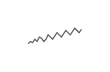
\begin{tikzpicture}[x=0.08em, y=0.08em, line width=0.4pt]
                \draw[FooterGray] (0,3) -- (1,4) -- (2,3.5) -- (3,5) -- (4,4) -- (5,6) -- (6,5.5) -- (7,4) -- (8,5) -- (9,7) -- (10,6) -- (11,5) -- (12,6.5) -- (13,8) -- (14,7) -- (15,6) -- (16,7.5) -- (17,9) -- (18,8) -- (19,7) -- (20,8.5) -- (21,10) -- (22,9) -- (23,8) -- (24,9.5);
            \end{tikzpicture}%
        }%
        \hskip0.5cm%
    }%
    \vskip6pt%
}

%=============================================================================
% PACKAGES
%=============================================================================
\usepackage[utf8]{inputenc}
\DeclareUnicodeCharacter{03B1}{\ensuremath{\alpha}}
\usepackage[T1]{fontenc}
\usepackage{amsmath, amssymb, amsthm}
\usepackage{mathtools}
\usepackage{bm}
\usepackage{tikz}
\usetikzlibrary{arrows.meta, positioning, shapes, calc, decorations.pathreplacing, shadings}
\usepackage{booktabs}
\usepackage{multirow}
\usepackage{array}
\usepackage{graphicx}
\usepackage{animate}
\usepackage{hyperref}
\usepackage{colortbl}
\usepackage{listings}
\lstset{language=Python, basicstyle=\ttfamily\scriptsize, keywordstyle=\color{MainBlue}\bfseries,
  commentstyle=\color{Forest}, stringstyle=\color{Crimson}, breaklines=true,
  frame=none, backgroundcolor=\color{VeryLightGray}, xleftmargin=2mm}
\hypersetup{colorlinks=true, linkcolor=MainBlue, urlcolor=MainBlue}
\graphicspath{{../../logos/}{../../charts/}{../../photos/}}
\usepackage{xcolor}
\hfuzz=2pt  % Suppress tiny overfull warnings (<2pt)
\vfuzz=2pt  % Suppress tiny vertical overfull warnings (<2pt)
% \mathrm in the sans-serif family of the slides (beamer resets \mathrm to the serif family at \begin{document};
% this hook runs after beamer's, so WN, Var, RMSE, ... in formulas match the surrounding text)
% Bold vectors and matrices in the same sans-serif family: \mathbf{A} in sans bold (beamer's own \mathbf came out in
% medium weight), and the bold upright Greek capitals of \boldsymbol / \bm (\bSigma, \bPhi, \boldsymbol{\Theta}) in
% cmss bold: bm.sty fixes its "boldoperators" font when it is loaded (serif cmbx), before beamer switches the
% operators to cmss, so it is reset here.
\AtBeginDocument{%
  \SetMathAlphabet{\mathrm}{normal}{\encodingdefault}{\sfdefault}{\mddefault}{n}%
  \SetMathAlphabet{\mathrm}{bold}{\encodingdefault}{\sfdefault}{bx}{n}%
  \SetMathAlphabet{\mathbf}{normal}{\encodingdefault}{\sfdefault}{bx}{n}%
  \SetMathAlphabet{\mathbf}{bold}{\encodingdefault}{\sfdefault}{bx}{n}%
  \SetSymbolFont{boldoperators}{normal}{OT1}{cmss}{bx}{n}%
  \SetSymbolFont{boldoperators}{bold}{OT1}{cmss}{bx}{n}}

%=============================================================================
% QUANTLET COMMANDS
%   \quantlet{<displayed name>}{<url>}       (generic, compatible with the older TSA decks)
%   \tsaquantlet{Ch_05}{TSA_ch5_garch}       -> https://github.com/danpele/Time-Series-Analysis/tree/main/Quantlets/Ch_05/TSA_ch5_garch
%   \qlurl{<folder>} is defined per chapter by the generator (Quantlets/Ch_NN/<folder>)
%=============================================================================
\newcommand{\tsarepo}{https://github.com/danpele/Time-Series-Analysis}
\newcommand{\tsaqlbase}{https://github.com/danpele/Time-Series-Analysis/tree/main/Quantlets}
\newcommand{\quantlet}[2]{%
    \hfill\href{#2}{%
        \raisebox{-0.15em}{
\includegraphics[height=0.7em]{ql_logo.png}}%
        \textcolor{MainBlue}{\tiny\ #1}%
    }%
}
\newcommand{\tsaquantlet}[2]{\quantlet{\detokenize{#2}}{\tsaqlbase/#1/#2}}

%=============================================================================
% NOTEBOOKS (Google Colab)
%   \colaburl{notebooks/EN/chapter5_seminar_notebook.ipynb} -> the Colab link of a file in the TSA repo
%   \nb: the chapter notebook (each seminar deck redefines it with \renewcommand)
%=============================================================================
\newcommand{\colaburl}[1]{https://colab.research.google.com/github/danpele/Time-Series-Analysis/blob/main/#1}
\newcommand{\nb}{https://colab.research.google.com/github/danpele/Time-Series-Analysis/tree/main/notebooks/EN}
\newcommand{\nbname}{notebooks/EN}

%=============================================================================
% SLIDE HELPERS (used by the generators; the same as in MFM)
%=============================================================================
% local font size for list bodies (the preamble forces \normalsize)
\newcommand{\itemsize}[1]{\setbeamertemplate{itemize/enumerate body begin}{#1}\setbeamertemplate{itemize/enumerate subbody begin}{#1}}
\newcommand{\intitle}[1]{{\hypersetup{urlcolor=white}#1}}   % white links inside coloured title bars
\newcommand{\imgcap}[1]{{\scriptsize #1}\\[0.5mm]}          % caption under a photo
\newcommand{\imgcredit}[2]{{\tiny\color{FooterGray}\href{#1}{#2}}}   % image credit: source URL, author/licence
\newcommand{\aiprompt}[1]{{\ttfamily\color{MainBlue}#1}}     % a prompt to an AI assistant

%=============================================================================
% SEMINARS: student version by default; the instructor wrapper *_solutions.tex sets \solutionstrue
%=============================================================================
\makeatletter\@ifundefined{ifsolutions}{\expandafter\newif\csname ifsolutions\endcsname}{}\makeatother
\newcommand{\solonly}[1]{\ifsolutions #1\fi}
\newcommand{\propsub}{\ifsolutions\else\framesubtitle{\ifdefined\tsalang Rezolvarea se discută la seminar\else Solution discussed in class\fi}\fi}

%=============================================================================
% APPENDIX AND CHAPTER LINKS (latex/appendix_links.py writes the calls; it also re-declares these
% macros before \begin{document}, so the decks compile with or without this preamble block)
%=============================================================================
\providecommand{\tsaapplink}[3]{\hypertarget{#2}{}\hyperlink{#1}{\beamergotobutton{#3}}}
\providecommand{\tsaappback}[2]{\begin{tikzpicture}[remember picture,overlay]\node[anchor=south east] at ([xshift=-3mm,yshift=7mm]current page.south east){\hyperlink{#1}{\beamerreturnbutton{#2}}};\end{tikzpicture}}
\providecommand{\tsachlink}[2]{\href{#1}{#2}}
\providecommand{\tsachlinkt}[2]{\href{#1}{\usebeamercolor[fg]{frametitle}#2}}

%=============================================================================
% QUANTINAR COMMAND: link către un curs Quantinar (subiecte avansate)
%=============================================================================
\newcommand{\quantinar}[2]{%
    \href{#2}{%
        \raisebox{-0.15em}{
\includegraphics[height=0.8em]{qr_logo.png}}%
        \textcolor{MainBlue}{\scriptsize\ #1}%
    }%
}

%=============================================================================
% CUSTOM TITLE PAGE
%=============================================================================
\defbeamertemplate*{title page}{hybrid}[1][]
{
    \vspace{0.2cm}
    % Logos row - top header (with clickable links)
    \begin{center}
        \href{https://www.ase.ro}{
\includegraphics[height=1.0cm]{ase_logo.png}}\hspace{0.3cm}%
        \href{https://theida.net}{
\includegraphics[height=1.0cm]{ida_logo.png}}\hspace{0.3cm}%
        \href{https://blockchain-research-center.com}{
\includegraphics[height=1.0cm]{brc_logo.png}}\hspace{0.3cm}%
        \href{https://www.ai4efin.ase.ro}{
\includegraphics[height=1.0cm]{ai4efin_logo.png}}\hspace{0.3cm}%
        \href{https://ipe.ro/new}{
\includegraphics[height=1.0cm]{acad_logo.png}}\hspace{0.3cm}%
        \href{https://www.digital-finance-msca.com}{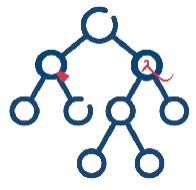
\includegraphics[height=1.0cm]{msca_logo.png}}%
    \end{center}

    \vspace{0.6cm}

    % Main title with Q logos on sides (with clickable links)
    \begin{center}
        \begin{minipage}{0.1\textwidth}
            \centering
            \href{https://quantlet.com}{
\includegraphics[height=1.1cm]{ql_logo.png}}
        \end{minipage}%
        \begin{minipage}{0.78\textwidth}
            \centering
            {\LARGE\bfseries\usebeamercolor[fg]{title}\inserttitle}

            \vspace{0.3cm}

            {\usebeamerfont{subtitle}\usebeamercolor[fg]{title}\insertsubtitle}
        \end{minipage}%
        \begin{minipage}{0.1\textwidth}
            \centering
            \href{https://quantinar.com}{
\includegraphics[height=1.1cm]{qr_logo.png}}
        \end{minipage}
    \end{center}

    \vspace{0.6cm}

    % Authors (left aligned)
    \hspace{0.5cm}{\usebeamerfont{author}\insertauthor}

    \vspace{0.3cm}

    % Institute/Affiliations (left aligned)
    \hspace{0.5cm}\begin{minipage}[t]{0.9\textwidth}
        \raggedright\small\insertinstitute
    \end{minipage}
}

%=============================================================================
% THEOREM ENVIRONMENTS
%=============================================================================
\theoremstyle{definition}
\setbeamertemplate{theorems}[numbered]
\ifdefined\tsalang
\newtheorem{defn}{Definiție}
\newtheorem{thm}{Teoremă}
\newtheorem{prop}{Propoziție}
\newtheorem{rmk}{Observație}
\else
\newtheorem{defn}{Definition}
\newtheorem{thm}{Theorem}
\newtheorem{prop}{Proposition}
\newtheorem{rmk}{Remark}
\fi

%=============================================================================
% CENTRED MINIPAGE (no extra vertical space)
%=============================================================================
\newenvironment{cminipage}[1]{%
    \par\noindent\hfill\begin{minipage}{#1}\ignorespaces
}{%
    \end{minipage}\hfill\null\par
}

%=============================================================================
% CUSTOM COMMANDS
%=============================================================================
\newcommand{\E}{\mathbb{E}}
\newcommand{\Var}{\text{Var}}
\newcommand{\Cov}{\text{Cov}}
\newcommand{\Corr}{\text{Corr}}
\newcommand{\R}{\mathbb{R}}
\newcommand{\N}{\mathbb{N}}
\newcommand{\Z}{\mathbb{Z}}
\newcommand{\B}{\mathbf{B}}
\newcommand{\imark}{\textcolor{MainBlue}{\textbullet}}
\newcommand{\RMSE}{\text{RMSE}}
\newcommand{\MAE}{\text{MAE}}
\newcommand{\MAPE}{\text{MAPE}}

% Boldface vector/matrix commands (VAR, VECM, state space; also used by the older TSA decks)
\newcommand{\bY}{\mathbf{Y}}
\newcommand{\bX}{\mathbf{X}}
\newcommand{\bA}{\mathbf{A}}
\newcommand{\bB}{\mathbf{B}}
\newcommand{\bepsilon}{\boldsymbol{\varepsilon}}
\newcommand{\bSigma}{\boldsymbol{\Sigma}}
\newcommand{\bPhi}{\boldsymbol{\Phi}}
\newcommand{\bGamma}{\boldsymbol{\Gamma}}
\newcommand{\bPi}{\boldsymbol{\Pi}}
\newcommand{\bc}{\mathbf{c}}
\newcommand{\balpha}{\boldsymbol{\alpha}}
\newcommand{\bbeta}{\boldsymbol{\beta}}
\newcommand{\bvarepsilon}{\boldsymbol{\varepsilon}}

% Legacy seminar marks (older TSA seminar decks)
\newcommand{\correct}{\textcolor{Forest}{\checkmark}}
\newcommand{\incorrect}{\textcolor{Crimson}{\texttimes}}
 se definește
%   \newcommand{\coursename}{Time Series Analysis}      (EN)
%   \newcommand{\coursename}{Serii de timp}       (RO)  și  \def\tsalang{ro}
% Fișierele .tex se află în EN/Courses, EN/Seminars, RO/Cursuri, RO/Seminarii (două niveluri sub rădăcină).
% Deck-urile sînt generate de latex/build_chapterN.py / build_seminarN.py (vezi latex/tsa_build.py).

\documentclass[9pt, aspectratio=169, t]{beamer}
\providecommand{\coursename}{Time Series Analysis}

% Ensure content fits on slides
\setbeamersize{text margin left=8mm, text margin right=8mm}
% Smaller institute font (title page)
\setbeamerfont{institute}{size=\footnotesize}

%=============================================================================
% THEME AND STYLE CONFIGURATION
%=============================================================================
\usetheme{default}
% Using default theme for clean header/footer control

% Color Palette (matching Redispatch PDF)
\definecolor{MainBlue}{RGB}{26, 58, 110}
\definecolor{AccentBlue}{RGB}{26, 58, 110}
\definecolor{IDAred}{RGB}{205, 0, 0}
\definecolor{DarkGray}{RGB}{51, 51, 51}
\definecolor{MediumGray}{RGB}{128, 128, 128}
\definecolor{LightGray}{RGB}{248, 248, 248}
\definecolor{VeryLightGray}{RGB}{235, 235, 235}
\definecolor{KeynoteGray}{RGB}{218, 218, 218}
\definecolor{SectionGray}{RGB}{120, 120, 120}
\definecolor{FooterGray}{RGB}{100, 100, 100}
\definecolor{Crimson}{RGB}{220, 53, 69}
\definecolor{Forest}{RGB}{46, 125, 50}
\definecolor{Amber}{RGB}{181, 133, 63}
\definecolor{Orange}{RGB}{230, 126, 34}
\definecolor{Purple}{RGB}{142, 68, 173}

% Gradient background (exact Keynote 315° gradient: white to RGB 218,218,218)
\setbeamertemplate{background}{%
    \begin{tikzpicture}[remember picture, overlay]
        \shade[shading=axis, shading angle=315,
        top color=white, bottom color=KeynoteGray]
        (current page.south west) rectangle (current page.north east);
    \end{tikzpicture}%
}
% Fallback solid color for compatibility
\setbeamercolor{background canvas}{bg=}

\setbeamercolor{palette primary}{bg=MainBlue, fg=white}
\setbeamercolor{palette secondary}{bg=MainBlue!85, fg=white}
\setbeamercolor{palette tertiary}{bg=MainBlue!70, fg=white}
\setbeamercolor{structure}{fg=MainBlue}
\setbeamercolor{title}{fg=IDAred}
\setbeamercolor{frametitle}{fg=IDAred, bg=}
\setbeamercolor{block title}{bg=MainBlue, fg=white}
\setbeamercolor{block body}{bg=VeryLightGray, fg=DarkGray}
\setbeamercolor{block title alerted}{bg=Crimson, fg=white}
\setbeamercolor{block body alerted}{bg=Crimson!8, fg=DarkGray}
\setbeamercolor{block title example}{bg=Forest, fg=white}
\setbeamercolor{block body example}{bg=Forest!8, fg=DarkGray}
\setbeamercolor{item}{fg=MainBlue}

% Footer colors (override Madrid theme blue)
\setbeamercolor{author in head/foot}{fg=FooterGray, bg=}
\setbeamercolor{title in head/foot}{fg=FooterGray, bg=}
\setbeamercolor{date in head/foot}{fg=FooterGray, bg=}
\setbeamercolor{section in head/foot}{fg=FooterGray, bg=}
\setbeamercolor{subsection in head/foot}{fg=FooterGray, bg=}

% Bullet styles (apply everywhere including blocks)
\setbeamertemplate{itemize item}{\color{MainBlue}$\boxdot$}
\setbeamertemplate{itemize subitem}{\color{MainBlue}$\blacktriangleright$}
\setbeamertemplate{itemize subsubitem}{\color{MainBlue}\tiny$\bullet$}
\setbeamertemplate{itemize/enumerate body begin}{\normalsize}
\setbeamertemplate{itemize/enumerate subbody begin}{\normalsize}

% Item spacing - compact style
\setlength{\leftmargini}{10pt}       % Level 1: minimal indent
\setlength{\leftmarginii}{10pt}      % Level 2: minimal additional indent
% Compact list spacing (zero extra space before/after lists in blocks)
\makeatletter
\def\@listi{\leftmargin\leftmargini \topsep 0pt \parsep 0pt \itemsep 0pt}
\def\@listii{\leftmargin\leftmarginii \topsep 0pt \parsep 0pt \itemsep 0pt}
\makeatother

\setbeamertemplate{navigation symbols}{}

%=============================================================================
% CUSTOM HEADLINE
%=============================================================================
\setbeamertemplate{headline}{%
    \vskip10pt%
    \hbox to \paperwidth{%
        \hskip0.5cm%
        {\small\color{FooterGray}\renewcommand{\hyperlink}[2]{##2}\insertsectionhead}%
        \hfill%
        \textcolor{FooterGray}{\small\insertframenumber}%
        \hskip0.5cm%
    }%
    \vskip4pt%
    {\color{FooterGray}\hrule height 0.4pt}%
}

%=============================================================================
% CUSTOM FOOTER
%=============================================================================
\usepackage{fontawesome5}

\setbeamertemplate{footline}{%
    {\color{FooterGray}\hrule height 0.4pt}%
    \vskip4pt%
    \hbox to \paperwidth{%
        \hskip0.5cm%
        \textcolor{FooterGray}{\small\coursename}%
        \hfill%
        \raisebox{-0.1em}{%
            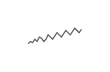
\begin{tikzpicture}[x=0.08em, y=0.08em, line width=0.4pt]
                \draw[FooterGray] (0,3) -- (1,4) -- (2,3.5) -- (3,5) -- (4,4) -- (5,6) -- (6,5.5) -- (7,4) -- (8,5) -- (9,7) -- (10,6) -- (11,5) -- (12,6.5) -- (13,8) -- (14,7) -- (15,6) -- (16,7.5) -- (17,9) -- (18,8) -- (19,7) -- (20,8.5) -- (21,10) -- (22,9) -- (23,8) -- (24,9.5);
            \end{tikzpicture}%
        }%
        \hskip0.5cm%
    }%
    \vskip6pt%
}

%=============================================================================
% PACKAGES
%=============================================================================
\usepackage[utf8]{inputenc}
\DeclareUnicodeCharacter{03B1}{\ensuremath{\alpha}}
\usepackage[T1]{fontenc}
\usepackage{amsmath, amssymb, amsthm}
\usepackage{mathtools}
\usepackage{bm}
\usepackage{tikz}
\usetikzlibrary{arrows.meta, positioning, shapes, calc, decorations.pathreplacing, shadings}
\usepackage{booktabs}
\usepackage{multirow}
\usepackage{array}
\usepackage{graphicx}
\usepackage{animate}
\usepackage{hyperref}
\usepackage{colortbl}
\usepackage{listings}
\lstset{language=Python, basicstyle=\ttfamily\scriptsize, keywordstyle=\color{MainBlue}\bfseries,
  commentstyle=\color{Forest}, stringstyle=\color{Crimson}, breaklines=true,
  frame=none, backgroundcolor=\color{VeryLightGray}, xleftmargin=2mm}
\hypersetup{colorlinks=true, linkcolor=MainBlue, urlcolor=MainBlue}
\graphicspath{{../../logos/}{../../charts/}{../../photos/}}
\usepackage{xcolor}
\hfuzz=2pt  % Suppress tiny overfull warnings (<2pt)
\vfuzz=2pt  % Suppress tiny vertical overfull warnings (<2pt)
% \mathrm in the sans-serif family of the slides (beamer resets \mathrm to the serif family at \begin{document};
% this hook runs after beamer's, so WN, Var, RMSE, ... in formulas match the surrounding text)
% Bold vectors and matrices in the same sans-serif family: \mathbf{A} in sans bold (beamer's own \mathbf came out in
% medium weight), and the bold upright Greek capitals of \boldsymbol / \bm (\bSigma, \bPhi, \boldsymbol{\Theta}) in
% cmss bold: bm.sty fixes its "boldoperators" font when it is loaded (serif cmbx), before beamer switches the
% operators to cmss, so it is reset here.
\AtBeginDocument{%
  \SetMathAlphabet{\mathrm}{normal}{\encodingdefault}{\sfdefault}{\mddefault}{n}%
  \SetMathAlphabet{\mathrm}{bold}{\encodingdefault}{\sfdefault}{bx}{n}%
  \SetMathAlphabet{\mathbf}{normal}{\encodingdefault}{\sfdefault}{bx}{n}%
  \SetMathAlphabet{\mathbf}{bold}{\encodingdefault}{\sfdefault}{bx}{n}%
  \SetSymbolFont{boldoperators}{normal}{OT1}{cmss}{bx}{n}%
  \SetSymbolFont{boldoperators}{bold}{OT1}{cmss}{bx}{n}}

%=============================================================================
% QUANTLET COMMANDS
%   \quantlet{<displayed name>}{<url>}       (generic, compatible with the older TSA decks)
%   \tsaquantlet{Ch_05}{TSA_ch5_garch}       -> https://github.com/danpele/Time-Series-Analysis/tree/main/Quantlets/Ch_05/TSA_ch5_garch
%   \qlurl{<folder>} is defined per chapter by the generator (Quantlets/Ch_NN/<folder>)
%=============================================================================
\newcommand{\tsarepo}{https://github.com/danpele/Time-Series-Analysis}
\newcommand{\tsaqlbase}{https://github.com/danpele/Time-Series-Analysis/tree/main/Quantlets}
\newcommand{\quantlet}[2]{%
    \hfill\href{#2}{%
        \raisebox{-0.15em}{
\includegraphics[height=0.7em]{ql_logo.png}}%
        \textcolor{MainBlue}{\tiny\ #1}%
    }%
}
\newcommand{\tsaquantlet}[2]{\quantlet{\detokenize{#2}}{\tsaqlbase/#1/#2}}

%=============================================================================
% NOTEBOOKS (Google Colab)
%   \colaburl{notebooks/EN/chapter5_seminar_notebook.ipynb} -> the Colab link of a file in the TSA repo
%   \nb: the chapter notebook (each seminar deck redefines it with \renewcommand)
%=============================================================================
\newcommand{\colaburl}[1]{https://colab.research.google.com/github/danpele/Time-Series-Analysis/blob/main/#1}
\newcommand{\nb}{https://colab.research.google.com/github/danpele/Time-Series-Analysis/tree/main/notebooks/EN}
\newcommand{\nbname}{notebooks/EN}

%=============================================================================
% SLIDE HELPERS (used by the generators; the same as in MFM)
%=============================================================================
% local font size for list bodies (the preamble forces \normalsize)
\newcommand{\itemsize}[1]{\setbeamertemplate{itemize/enumerate body begin}{#1}\setbeamertemplate{itemize/enumerate subbody begin}{#1}}
\newcommand{\intitle}[1]{{\hypersetup{urlcolor=white}#1}}   % white links inside coloured title bars
\newcommand{\imgcap}[1]{{\scriptsize #1}\\[0.5mm]}          % caption under a photo
\newcommand{\imgcredit}[2]{{\tiny\color{FooterGray}\href{#1}{#2}}}   % image credit: source URL, author/licence
\newcommand{\aiprompt}[1]{{\ttfamily\color{MainBlue}#1}}     % a prompt to an AI assistant

%=============================================================================
% SEMINARS: student version by default; the instructor wrapper *_solutions.tex sets \solutionstrue
%=============================================================================
\makeatletter\@ifundefined{ifsolutions}{\expandafter\newif\csname ifsolutions\endcsname}{}\makeatother
\newcommand{\solonly}[1]{\ifsolutions #1\fi}
\newcommand{\propsub}{\ifsolutions\else\framesubtitle{\ifdefined\tsalang Rezolvarea se discută la seminar\else Solution discussed in class\fi}\fi}

%=============================================================================
% APPENDIX AND CHAPTER LINKS (latex/appendix_links.py writes the calls; it also re-declares these
% macros before \begin{document}, so the decks compile with or without this preamble block)
%=============================================================================
\providecommand{\tsaapplink}[3]{\hypertarget{#2}{}\hyperlink{#1}{\beamergotobutton{#3}}}
\providecommand{\tsaappback}[2]{\begin{tikzpicture}[remember picture,overlay]\node[anchor=south east] at ([xshift=-3mm,yshift=7mm]current page.south east){\hyperlink{#1}{\beamerreturnbutton{#2}}};\end{tikzpicture}}
\providecommand{\tsachlink}[2]{\href{#1}{#2}}
\providecommand{\tsachlinkt}[2]{\href{#1}{\usebeamercolor[fg]{frametitle}#2}}

%=============================================================================
% QUANTINAR COMMAND: link către un curs Quantinar (subiecte avansate)
%=============================================================================
\newcommand{\quantinar}[2]{%
    \href{#2}{%
        \raisebox{-0.15em}{
\includegraphics[height=0.8em]{qr_logo.png}}%
        \textcolor{MainBlue}{\scriptsize\ #1}%
    }%
}

%=============================================================================
% CUSTOM TITLE PAGE
%=============================================================================
\defbeamertemplate*{title page}{hybrid}[1][]
{
    \vspace{0.2cm}
    % Logos row - top header (with clickable links)
    \begin{center}
        \href{https://www.ase.ro}{
\includegraphics[height=1.0cm]{ase_logo.png}}\hspace{0.3cm}%
        \href{https://theida.net}{
\includegraphics[height=1.0cm]{ida_logo.png}}\hspace{0.3cm}%
        \href{https://blockchain-research-center.com}{
\includegraphics[height=1.0cm]{brc_logo.png}}\hspace{0.3cm}%
        \href{https://www.ai4efin.ase.ro}{
\includegraphics[height=1.0cm]{ai4efin_logo.png}}\hspace{0.3cm}%
        \href{https://ipe.ro/new}{
\includegraphics[height=1.0cm]{acad_logo.png}}\hspace{0.3cm}%
        \href{https://www.digital-finance-msca.com}{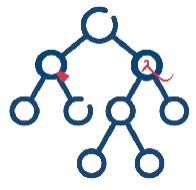
\includegraphics[height=1.0cm]{msca_logo.png}}%
    \end{center}

    \vspace{0.6cm}

    % Main title with Q logos on sides (with clickable links)
    \begin{center}
        \begin{minipage}{0.1\textwidth}
            \centering
            \href{https://quantlet.com}{
\includegraphics[height=1.1cm]{ql_logo.png}}
        \end{minipage}%
        \begin{minipage}{0.78\textwidth}
            \centering
            {\LARGE\bfseries\usebeamercolor[fg]{title}\inserttitle}

            \vspace{0.3cm}

            {\usebeamerfont{subtitle}\usebeamercolor[fg]{title}\insertsubtitle}
        \end{minipage}%
        \begin{minipage}{0.1\textwidth}
            \centering
            \href{https://quantinar.com}{
\includegraphics[height=1.1cm]{qr_logo.png}}
        \end{minipage}
    \end{center}

    \vspace{0.6cm}

    % Authors (left aligned)
    \hspace{0.5cm}{\usebeamerfont{author}\insertauthor}

    \vspace{0.3cm}

    % Institute/Affiliations (left aligned)
    \hspace{0.5cm}\begin{minipage}[t]{0.9\textwidth}
        \raggedright\small\insertinstitute
    \end{minipage}
}

%=============================================================================
% THEOREM ENVIRONMENTS
%=============================================================================
\theoremstyle{definition}
\setbeamertemplate{theorems}[numbered]
\ifdefined\tsalang
\newtheorem{defn}{Definiție}
\newtheorem{thm}{Teoremă}
\newtheorem{prop}{Propoziție}
\newtheorem{rmk}{Observație}
\else
\newtheorem{defn}{Definition}
\newtheorem{thm}{Theorem}
\newtheorem{prop}{Proposition}
\newtheorem{rmk}{Remark}
\fi

%=============================================================================
% CENTRED MINIPAGE (no extra vertical space)
%=============================================================================
\newenvironment{cminipage}[1]{%
    \par\noindent\hfill\begin{minipage}{#1}\ignorespaces
}{%
    \end{minipage}\hfill\null\par
}

%=============================================================================
% CUSTOM COMMANDS
%=============================================================================
\newcommand{\E}{\mathbb{E}}
\newcommand{\Var}{\text{Var}}
\newcommand{\Cov}{\text{Cov}}
\newcommand{\Corr}{\text{Corr}}
\newcommand{\R}{\mathbb{R}}
\newcommand{\N}{\mathbb{N}}
\newcommand{\Z}{\mathbb{Z}}
\newcommand{\B}{\mathbf{B}}
\newcommand{\imark}{\textcolor{MainBlue}{\textbullet}}
\newcommand{\RMSE}{\text{RMSE}}
\newcommand{\MAE}{\text{MAE}}
\newcommand{\MAPE}{\text{MAPE}}

% Boldface vector/matrix commands (VAR, VECM, state space; also used by the older TSA decks)
\newcommand{\bY}{\mathbf{Y}}
\newcommand{\bX}{\mathbf{X}}
\newcommand{\bA}{\mathbf{A}}
\newcommand{\bB}{\mathbf{B}}
\newcommand{\bepsilon}{\boldsymbol{\varepsilon}}
\newcommand{\bSigma}{\boldsymbol{\Sigma}}
\newcommand{\bPhi}{\boldsymbol{\Phi}}
\newcommand{\bGamma}{\boldsymbol{\Gamma}}
\newcommand{\bPi}{\boldsymbol{\Pi}}
\newcommand{\bc}{\mathbf{c}}
\newcommand{\balpha}{\boldsymbol{\alpha}}
\newcommand{\bbeta}{\boldsymbol{\beta}}
\newcommand{\bvarepsilon}{\boldsymbol{\varepsilon}}

% Legacy seminar marks (older TSA seminar decks)
\newcommand{\correct}{\textcolor{Forest}{\checkmark}}
\newcommand{\incorrect}{\textcolor{Crimson}{\texttimes}}
 se definește
%   \newcommand{\coursename}{Time Series Analysis}      (EN)
%   \newcommand{\coursename}{Serii de timp}       (RO)  și  \def\tsalang{ro}
% Fișierele .tex se află în EN/Courses, EN/Seminars, RO/Cursuri, RO/Seminarii (două niveluri sub rădăcină).
% Deck-urile sînt generate de latex/build_chapterN.py / build_seminarN.py (vezi latex/tsa_build.py).

\documentclass[9pt, aspectratio=169, t]{beamer}
\providecommand{\coursename}{Time Series Analysis}

% Ensure content fits on slides
\setbeamersize{text margin left=8mm, text margin right=8mm}
% Smaller institute font (title page)
\setbeamerfont{institute}{size=\footnotesize}

%=============================================================================
% THEME AND STYLE CONFIGURATION
%=============================================================================
\usetheme{default}
% Using default theme for clean header/footer control

% Color Palette (matching Redispatch PDF)
\definecolor{MainBlue}{RGB}{26, 58, 110}
\definecolor{AccentBlue}{RGB}{26, 58, 110}
\definecolor{IDAred}{RGB}{205, 0, 0}
\definecolor{DarkGray}{RGB}{51, 51, 51}
\definecolor{MediumGray}{RGB}{128, 128, 128}
\definecolor{LightGray}{RGB}{248, 248, 248}
\definecolor{VeryLightGray}{RGB}{235, 235, 235}
\definecolor{KeynoteGray}{RGB}{218, 218, 218}
\definecolor{SectionGray}{RGB}{120, 120, 120}
\definecolor{FooterGray}{RGB}{100, 100, 100}
\definecolor{Crimson}{RGB}{220, 53, 69}
\definecolor{Forest}{RGB}{46, 125, 50}
\definecolor{Amber}{RGB}{181, 133, 63}
\definecolor{Orange}{RGB}{230, 126, 34}
\definecolor{Purple}{RGB}{142, 68, 173}

% Gradient background (exact Keynote 315° gradient: white to RGB 218,218,218)
\setbeamertemplate{background}{%
    \begin{tikzpicture}[remember picture, overlay]
        \shade[shading=axis, shading angle=315,
        top color=white, bottom color=KeynoteGray]
        (current page.south west) rectangle (current page.north east);
    \end{tikzpicture}%
}
% Fallback solid color for compatibility
\setbeamercolor{background canvas}{bg=}

\setbeamercolor{palette primary}{bg=MainBlue, fg=white}
\setbeamercolor{palette secondary}{bg=MainBlue!85, fg=white}
\setbeamercolor{palette tertiary}{bg=MainBlue!70, fg=white}
\setbeamercolor{structure}{fg=MainBlue}
\setbeamercolor{title}{fg=IDAred}
\setbeamercolor{frametitle}{fg=IDAred, bg=}
\setbeamercolor{block title}{bg=MainBlue, fg=white}
\setbeamercolor{block body}{bg=VeryLightGray, fg=DarkGray}
\setbeamercolor{block title alerted}{bg=Crimson, fg=white}
\setbeamercolor{block body alerted}{bg=Crimson!8, fg=DarkGray}
\setbeamercolor{block title example}{bg=Forest, fg=white}
\setbeamercolor{block body example}{bg=Forest!8, fg=DarkGray}
\setbeamercolor{item}{fg=MainBlue}

% Footer colors (override Madrid theme blue)
\setbeamercolor{author in head/foot}{fg=FooterGray, bg=}
\setbeamercolor{title in head/foot}{fg=FooterGray, bg=}
\setbeamercolor{date in head/foot}{fg=FooterGray, bg=}
\setbeamercolor{section in head/foot}{fg=FooterGray, bg=}
\setbeamercolor{subsection in head/foot}{fg=FooterGray, bg=}

% Bullet styles (apply everywhere including blocks)
\setbeamertemplate{itemize item}{\color{MainBlue}$\boxdot$}
\setbeamertemplate{itemize subitem}{\color{MainBlue}$\blacktriangleright$}
\setbeamertemplate{itemize subsubitem}{\color{MainBlue}\tiny$\bullet$}
\setbeamertemplate{itemize/enumerate body begin}{\normalsize}
\setbeamertemplate{itemize/enumerate subbody begin}{\normalsize}

% Item spacing - compact style
\setlength{\leftmargini}{10pt}       % Level 1: minimal indent
\setlength{\leftmarginii}{10pt}      % Level 2: minimal additional indent
% Compact list spacing (zero extra space before/after lists in blocks)
\makeatletter
\def\@listi{\leftmargin\leftmargini \topsep 0pt \parsep 0pt \itemsep 0pt}
\def\@listii{\leftmargin\leftmarginii \topsep 0pt \parsep 0pt \itemsep 0pt}
\makeatother

\setbeamertemplate{navigation symbols}{}

%=============================================================================
% CUSTOM HEADLINE
%=============================================================================
\setbeamertemplate{headline}{%
    \vskip10pt%
    \hbox to \paperwidth{%
        \hskip0.5cm%
        {\small\color{FooterGray}\renewcommand{\hyperlink}[2]{##2}\insertsectionhead}%
        \hfill%
        \textcolor{FooterGray}{\small\insertframenumber}%
        \hskip0.5cm%
    }%
    \vskip4pt%
    {\color{FooterGray}\hrule height 0.4pt}%
}

%=============================================================================
% CUSTOM FOOTER
%=============================================================================
\usepackage{fontawesome5}

\setbeamertemplate{footline}{%
    {\color{FooterGray}\hrule height 0.4pt}%
    \vskip4pt%
    \hbox to \paperwidth{%
        \hskip0.5cm%
        \textcolor{FooterGray}{\small\coursename}%
        \hfill%
        \raisebox{-0.1em}{%
            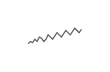
\begin{tikzpicture}[x=0.08em, y=0.08em, line width=0.4pt]
                \draw[FooterGray] (0,3) -- (1,4) -- (2,3.5) -- (3,5) -- (4,4) -- (5,6) -- (6,5.5) -- (7,4) -- (8,5) -- (9,7) -- (10,6) -- (11,5) -- (12,6.5) -- (13,8) -- (14,7) -- (15,6) -- (16,7.5) -- (17,9) -- (18,8) -- (19,7) -- (20,8.5) -- (21,10) -- (22,9) -- (23,8) -- (24,9.5);
            \end{tikzpicture}%
        }%
        \hskip0.5cm%
    }%
    \vskip6pt%
}

%=============================================================================
% PACKAGES
%=============================================================================
\usepackage[utf8]{inputenc}
\DeclareUnicodeCharacter{03B1}{\ensuremath{\alpha}}
\usepackage[T1]{fontenc}
\usepackage{amsmath, amssymb, amsthm}
\usepackage{mathtools}
\usepackage{bm}
\usepackage{tikz}
\usetikzlibrary{arrows.meta, positioning, shapes, calc, decorations.pathreplacing, shadings}
\usepackage{booktabs}
\usepackage{multirow}
\usepackage{array}
\usepackage{graphicx}
\usepackage{animate}
\usepackage{hyperref}
\usepackage{colortbl}
\usepackage{listings}
\lstset{language=Python, basicstyle=\ttfamily\scriptsize, keywordstyle=\color{MainBlue}\bfseries,
  commentstyle=\color{Forest}, stringstyle=\color{Crimson}, breaklines=true,
  frame=none, backgroundcolor=\color{VeryLightGray}, xleftmargin=2mm}
\hypersetup{colorlinks=true, linkcolor=MainBlue, urlcolor=MainBlue}
\graphicspath{{../../logos/}{../../charts/}{../../photos/}}
\usepackage{xcolor}
\hfuzz=2pt  % Suppress tiny overfull warnings (<2pt)
\vfuzz=2pt  % Suppress tiny vertical overfull warnings (<2pt)
% \mathrm in the sans-serif family of the slides (beamer resets \mathrm to the serif family at \begin{document};
% this hook runs after beamer's, so WN, Var, RMSE, ... in formulas match the surrounding text)
% Bold vectors and matrices in the same sans-serif family: \mathbf{A} in sans bold (beamer's own \mathbf came out in
% medium weight), and the bold upright Greek capitals of \boldsymbol / \bm (\bSigma, \bPhi, \boldsymbol{\Theta}) in
% cmss bold: bm.sty fixes its "boldoperators" font when it is loaded (serif cmbx), before beamer switches the
% operators to cmss, so it is reset here.
\AtBeginDocument{%
  \SetMathAlphabet{\mathrm}{normal}{\encodingdefault}{\sfdefault}{\mddefault}{n}%
  \SetMathAlphabet{\mathrm}{bold}{\encodingdefault}{\sfdefault}{bx}{n}%
  \SetMathAlphabet{\mathbf}{normal}{\encodingdefault}{\sfdefault}{bx}{n}%
  \SetMathAlphabet{\mathbf}{bold}{\encodingdefault}{\sfdefault}{bx}{n}%
  \SetSymbolFont{boldoperators}{normal}{OT1}{cmss}{bx}{n}%
  \SetSymbolFont{boldoperators}{bold}{OT1}{cmss}{bx}{n}}

%=============================================================================
% QUANTLET COMMANDS
%   \quantlet{<displayed name>}{<url>}       (generic, compatible with the older TSA decks)
%   \tsaquantlet{Ch_05}{TSA_ch5_garch}       -> https://github.com/danpele/Time-Series-Analysis/tree/main/Quantlets/Ch_05/TSA_ch5_garch
%   \qlurl{<folder>} is defined per chapter by the generator (Quantlets/Ch_NN/<folder>)
%=============================================================================
\newcommand{\tsarepo}{https://github.com/danpele/Time-Series-Analysis}
\newcommand{\tsaqlbase}{https://github.com/danpele/Time-Series-Analysis/tree/main/Quantlets}
\newcommand{\quantlet}[2]{%
    \hfill\href{#2}{%
        \raisebox{-0.15em}{
\includegraphics[height=0.7em]{ql_logo.png}}%
        \textcolor{MainBlue}{\tiny\ #1}%
    }%
}
\newcommand{\tsaquantlet}[2]{\quantlet{\detokenize{#2}}{\tsaqlbase/#1/#2}}

%=============================================================================
% NOTEBOOKS (Google Colab)
%   \colaburl{notebooks/EN/chapter5_seminar_notebook.ipynb} -> the Colab link of a file in the TSA repo
%   \nb: the chapter notebook (each seminar deck redefines it with \renewcommand)
%=============================================================================
\newcommand{\colaburl}[1]{https://colab.research.google.com/github/danpele/Time-Series-Analysis/blob/main/#1}
\newcommand{\nb}{https://colab.research.google.com/github/danpele/Time-Series-Analysis/tree/main/notebooks/EN}
\newcommand{\nbname}{notebooks/EN}

%=============================================================================
% SLIDE HELPERS (used by the generators; the same as in MFM)
%=============================================================================
% local font size for list bodies (the preamble forces \normalsize)
\newcommand{\itemsize}[1]{\setbeamertemplate{itemize/enumerate body begin}{#1}\setbeamertemplate{itemize/enumerate subbody begin}{#1}}
\newcommand{\intitle}[1]{{\hypersetup{urlcolor=white}#1}}   % white links inside coloured title bars
\newcommand{\imgcap}[1]{{\scriptsize #1}\\[0.5mm]}          % caption under a photo
\newcommand{\imgcredit}[2]{{\tiny\color{FooterGray}\href{#1}{#2}}}   % image credit: source URL, author/licence
\newcommand{\aiprompt}[1]{{\ttfamily\color{MainBlue}#1}}     % a prompt to an AI assistant

%=============================================================================
% SEMINARS: student version by default; the instructor wrapper *_solutions.tex sets \solutionstrue
%=============================================================================
\makeatletter\@ifundefined{ifsolutions}{\expandafter\newif\csname ifsolutions\endcsname}{}\makeatother
\newcommand{\solonly}[1]{\ifsolutions #1\fi}
\newcommand{\propsub}{\ifsolutions\else\framesubtitle{\ifdefined\tsalang Rezolvarea se discută la seminar\else Solution discussed in class\fi}\fi}

%=============================================================================
% APPENDIX AND CHAPTER LINKS (latex/appendix_links.py writes the calls; it also re-declares these
% macros before \begin{document}, so the decks compile with or without this preamble block)
%=============================================================================
\providecommand{\tsaapplink}[3]{\hypertarget{#2}{}\hyperlink{#1}{\beamergotobutton{#3}}}
\providecommand{\tsaappback}[2]{\begin{tikzpicture}[remember picture,overlay]\node[anchor=south east] at ([xshift=-3mm,yshift=7mm]current page.south east){\hyperlink{#1}{\beamerreturnbutton{#2}}};\end{tikzpicture}}
\providecommand{\tsachlink}[2]{\href{#1}{#2}}
\providecommand{\tsachlinkt}[2]{\href{#1}{\usebeamercolor[fg]{frametitle}#2}}

%=============================================================================
% QUANTINAR COMMAND: link către un curs Quantinar (subiecte avansate)
%=============================================================================
\newcommand{\quantinar}[2]{%
    \href{#2}{%
        \raisebox{-0.15em}{
\includegraphics[height=0.8em]{qr_logo.png}}%
        \textcolor{MainBlue}{\scriptsize\ #1}%
    }%
}

%=============================================================================
% CUSTOM TITLE PAGE
%=============================================================================
\defbeamertemplate*{title page}{hybrid}[1][]
{
    \vspace{0.2cm}
    % Logos row - top header (with clickable links)
    \begin{center}
        \href{https://www.ase.ro}{
\includegraphics[height=1.0cm]{ase_logo.png}}\hspace{0.3cm}%
        \href{https://theida.net}{
\includegraphics[height=1.0cm]{ida_logo.png}}\hspace{0.3cm}%
        \href{https://blockchain-research-center.com}{
\includegraphics[height=1.0cm]{brc_logo.png}}\hspace{0.3cm}%
        \href{https://www.ai4efin.ase.ro}{
\includegraphics[height=1.0cm]{ai4efin_logo.png}}\hspace{0.3cm}%
        \href{https://ipe.ro/new}{
\includegraphics[height=1.0cm]{acad_logo.png}}\hspace{0.3cm}%
        \href{https://www.digital-finance-msca.com}{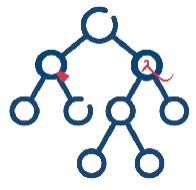
\includegraphics[height=1.0cm]{msca_logo.png}}%
    \end{center}

    \vspace{0.6cm}

    % Main title with Q logos on sides (with clickable links)
    \begin{center}
        \begin{minipage}{0.1\textwidth}
            \centering
            \href{https://quantlet.com}{
\includegraphics[height=1.1cm]{ql_logo.png}}
        \end{minipage}%
        \begin{minipage}{0.78\textwidth}
            \centering
            {\LARGE\bfseries\usebeamercolor[fg]{title}\inserttitle}

            \vspace{0.3cm}

            {\usebeamerfont{subtitle}\usebeamercolor[fg]{title}\insertsubtitle}
        \end{minipage}%
        \begin{minipage}{0.1\textwidth}
            \centering
            \href{https://quantinar.com}{
\includegraphics[height=1.1cm]{qr_logo.png}}
        \end{minipage}
    \end{center}

    \vspace{0.6cm}

    % Authors (left aligned)
    \hspace{0.5cm}{\usebeamerfont{author}\insertauthor}

    \vspace{0.3cm}

    % Institute/Affiliations (left aligned)
    \hspace{0.5cm}\begin{minipage}[t]{0.9\textwidth}
        \raggedright\small\insertinstitute
    \end{minipage}
}

%=============================================================================
% THEOREM ENVIRONMENTS
%=============================================================================
\theoremstyle{definition}
\setbeamertemplate{theorems}[numbered]
\ifdefined\tsalang
\newtheorem{defn}{Definiție}
\newtheorem{thm}{Teoremă}
\newtheorem{prop}{Propoziție}
\newtheorem{rmk}{Observație}
\else
\newtheorem{defn}{Definition}
\newtheorem{thm}{Theorem}
\newtheorem{prop}{Proposition}
\newtheorem{rmk}{Remark}
\fi

%=============================================================================
% CENTRED MINIPAGE (no extra vertical space)
%=============================================================================
\newenvironment{cminipage}[1]{%
    \par\noindent\hfill\begin{minipage}{#1}\ignorespaces
}{%
    \end{minipage}\hfill\null\par
}

%=============================================================================
% CUSTOM COMMANDS
%=============================================================================
\newcommand{\E}{\mathbb{E}}
\newcommand{\Var}{\text{Var}}
\newcommand{\Cov}{\text{Cov}}
\newcommand{\Corr}{\text{Corr}}
\newcommand{\R}{\mathbb{R}}
\newcommand{\N}{\mathbb{N}}
\newcommand{\Z}{\mathbb{Z}}
\newcommand{\B}{\mathbf{B}}
\newcommand{\imark}{\textcolor{MainBlue}{\textbullet}}
\newcommand{\RMSE}{\text{RMSE}}
\newcommand{\MAE}{\text{MAE}}
\newcommand{\MAPE}{\text{MAPE}}

% Boldface vector/matrix commands (VAR, VECM, state space; also used by the older TSA decks)
\newcommand{\bY}{\mathbf{Y}}
\newcommand{\bX}{\mathbf{X}}
\newcommand{\bA}{\mathbf{A}}
\newcommand{\bB}{\mathbf{B}}
\newcommand{\bepsilon}{\boldsymbol{\varepsilon}}
\newcommand{\bSigma}{\boldsymbol{\Sigma}}
\newcommand{\bPhi}{\boldsymbol{\Phi}}
\newcommand{\bGamma}{\boldsymbol{\Gamma}}
\newcommand{\bPi}{\boldsymbol{\Pi}}
\newcommand{\bc}{\mathbf{c}}
\newcommand{\balpha}{\boldsymbol{\alpha}}
\newcommand{\bbeta}{\boldsymbol{\beta}}
\newcommand{\bvarepsilon}{\boldsymbol{\varepsilon}}

% Legacy seminar marks (older TSA seminar decks)
\newcommand{\correct}{\textcolor{Forest}{\checkmark}}
\newcommand{\incorrect}{\textcolor{Crimson}{\texttimes}}


\newcommand{\qlurl}[1]{https://github.com/danpele/Time-Series-Analysis/tree/main/Quantlets/Ch_10/#1}

% Clickable citations (DOIs verified via Crossref)
\newcommand{\refHP}{\href{https://doi.org/10.1007/978-3-031-13584-2}{Huang și Petukhina (2022)}}
\newcommand{\refDK}{\href{https://doi.org/10.1093/acprof:oso/9780199641178.001.0001}{Durbin și Koopman (2012)}}
\newcommand{\refHarvey}{\href{https://doi.org/10.1017/CBO9781107049994}{Harvey (1989)}}
\newcommand{\refHamilton}{\href{https://doi.org/10.2307/j.ctv14jx6sm}{Hamilton (1994)}}
\newcommand{\refKN}{\href{https://doi.org/10.7551/mitpress/6444.001.0001}{Kim și Nelson (1999)}}
\newcommand{\refSS}{\href{https://doi.org/10.1007/978-3-319-52452-8}{Shumway și Stoffer (2017)}}
\newcommand{\refKalman}{\href{https://doi.org/10.1115/1.3662552}{Kalman (1960)}}
\newcommand{\refRTS}{\href{https://doi.org/10.2514/3.3166}{Rauch, Tung și Striebel (1965)}}
\newcommand{\refMuth}{\href{https://doi.org/10.1080/01621459.1960.10482064}{Muth (1960)}}
\newcommand{\refHKOS}{\href{https://doi.org/10.1007/978-3-540-71918-2}{Hyndman et al.\ (2008)}}
\newcommand{\refHJ}{\href{https://doi.org/10.1002/jae.3950080302}{Harvey și Jaeger (1993)}}
\newcommand{\refHPf}{\href{https://doi.org/10.2307/2953682}{Hodrick și Prescott (1997)}}
\newcommand{\refHamHP}{\href{https://doi.org/10.1162/rest\_a\_00706}{Hamilton (2018)}}
\newcommand{\refSW}{\href{https://doi.org/10.1086/654119}{Stock și Watson (1989)}}
\newcommand{\refGRS}{\href{https://doi.org/10.1016/j.jmoneco.2008.05.010}{Giannone, Reichlin și Small (2008)}}
\newcommand{\refHamMS}{\href{https://doi.org/10.2307/1912559}{Hamilton (1989)}}
\newcommand{\refHamEM}{\href{https://doi.org/10.1016/0304-4076(90)90093-9}{Hamilton (1990)}}
\newcommand{\refKim}{\href{https://doi.org/10.1016/0304-4076(94)90036-1}{Kim (1994)}}
\newcommand{\refCP}{\href{https://doi.org/10.1198/073500107000000296}{Chauvet și Piger (2008)}}
\newcommand{\refHSus}{\href{https://doi.org/10.1016/0304-4076(94)90067-1}{Hamilton și Susmel (1994)}}
\newcommand{\refLL}{\href{https://doi.org/10.1080/07350015.1990.10509794}{Lamoureux și Lastrapes (1990)}}
\newcommand{\refDI}{\href{https://doi.org/10.1016/S0304-4076(01)00073-2}{Diebold și Inoue (2001)}}

\title[Serii de timp]{Serii de timp}
\subtitle{Capitolul 10: Modele în spațiul stărilor, filtrul Kalman și modele Markov switching}
\author[D.T. Pele]{Daniel Traian PELE}
\institute{Academia de Studii Economice din București\\
IDA Institute Digital Assets\\
Blockchain Research Center\\
AI4EFin Artificial Intelligence for Energy Finance\\
Academia Română, Institutul de Prognoză Economică\\
MSCA Digital Finance}
\date{}

%=============================================================================
\providecommand{\tsaapplink}[3]{\hypertarget{#2}{}\hyperlink{#1}{\beamergotobutton{#3}}}  % APPLINKS-MACROS
\providecommand{\tsaappback}[2]{\begin{tikzpicture}[remember picture,overlay]\node[anchor=south east] at ([xshift=-3mm,yshift=7mm]current page.south east){\hyperlink{#1}{\beamerreturnbutton{#2}}};\end{tikzpicture}}  % APPLINKS-MACROS
\providecommand{\tsachlink}[2]{\href{#1}{#2}}  % APPLINKS-MACROS
\providecommand{\tsachlinkt}[2]{\href{#1}{\usebeamercolor[fg]{frametitle}#2}}  % APPLINKS-MACROS
\begin{document}
%=============================================================================

{
\setbeamertemplate{headline}{}
\setbeamertemplate{footline}{}
\begin{frame}[noframenumbering]
    \titlepage
\end{frame}
}
% BEGIN-ACRONYMS (generat de latex/acronyms.py; nu editati manual)
\begin{frame}{Acronime folosite în acest material (1/2)}
\setbeamertemplate{itemize/enumerate body begin}{\footnotesize}
\begin{columns}[T]
\begin{column}{0.49\textwidth}
\begin{itemize}\setlength{\itemsep}{0pt}
    \item \textbf{ACF}: Autocorrelation Function (funcția de autocorelație)
    \item \textbf{AI}: Artificial Intelligence (inteligență artificială)
    \item \textbf{AIC}: Akaike Information Criterion (criteriul informațional Akaike)
    \item \textbf{AR}: AutoRegressive (model) — model autoregresiv
    \item \textbf{ARCH}: AutoRegressive Conditional Heteroskedasticity (heteroscedasticitate condiționată autoregresivă)
    \item \textbf{ARIMA}: AutoRegressive Integrated Moving Average (model) — model autoregresiv integrat cu medie mobilă
    \item \textbf{ARMA}: AutoRegressive Moving Average (model) — model autoregresiv cu medie mobilă
    \item \textbf{BET}: Bucharest Exchange Trading (index) — indicele de referință al Bursei de Valori București
\end{itemize}
\end{column}
\begin{column}{0.49\textwidth}
\begin{itemize}\setlength{\itemsep}{0pt}
    \item \textbf{BIC}: Bayesian Information Criterion (criteriul informațional bayesian al lui Schwarz)
    \item \textbf{EM}: Expectation–Maximisation (algorithm) — algoritmul așteptare–maximizare
    \item \textbf{EODHD}: EOD Historical Data (market-data provider) — furnizor de date de piață
    \item \textbf{ETS}: Error, Trend, Seasonality (exponential smoothing state space models) — eroare, trend, sezonalitate (modele de netezire exponențială)
    \item \textbf{FRED}: Federal Reserve Economic Data (baza de date economice a Rezervei Federale din St. Louis)
    \item \textbf{GARCH}: Generalised AutoRegressive Conditional Heteroskedasticity (heteroscedasticitate condiționată autoregresivă generalizată)
    \item \textbf{GDP}: Gross Domestic Product (produsul intern brut)
\end{itemize}
\end{column}
\end{columns}
\end{frame}
\begin{frame}{Acronime folosite în acest material (2/2)}
\setbeamertemplate{itemize/enumerate body begin}{\footnotesize}
\begin{columns}[T]
\begin{column}{0.49\textwidth}
\begin{itemize}\setlength{\itemsep}{0pt}
    \item \textbf{HP}: Hodrick–Prescott (filter) — filtrul Hodrick–Prescott
    \item \textbf{IGARCH}: Integrated GARCH (GARCH integrat)
    \item \textbf{MA}: Moving Average (medie mobilă)
    \item \textbf{ML}: Machine Learning (învățare automată)
    \item \textbf{MS-AR}: Markov-Switching AutoRegressive (model) — model autoregresiv cu schimbare de regim de tip Markov
    \item \textbf{NASA}: National Aeronautics and Space Administration (agenția spațială a SUA)
    \item \textbf{NBER}: National Bureau of Economic Research (biroul național de cercetare economică al SUA, care datează recesiunile)
    \item \textbf{OLS}: Ordinary Least Squares (metoda celor mai mici pătrate)
    \item \textbf{PIB}: Produsul intern brut
\end{itemize}
\end{column}
\begin{column}{0.49\textwidth}
\begin{itemize}\setlength{\itemsep}{0pt}
    \item \textbf{RTS}: Rauch–Tung–Striebel (smoother) — netezitorul Rauch–Tung–Striebel
    \item \textbf{SD}: Standard Deviation (abaterea standard)
    \item \textbf{SES}: Simple Exponential Smoothing (netezire exponențială simplă)
    \item \textbf{SUA}: Statele Unite ale Americii
    \item \textbf{SWARCH}: Switching ARCH (model ARCH cu schimbare de regim)
    \item \textbf{TVP}: Time-Varying Parameter (regression) — regresie cu parametri variabili în timp
    \item \textbf{UC}: Unobserved Components (model) — model cu componente neobservate
    \item \textbf{UE}: Uniunea Europeană
    \item \textbf{VAR}: Vector AutoRegression (model vector autoregresiv)
\end{itemize}
\end{column}
\end{columns}
\end{frame}
% END-ACRONYMS

\begin{frame}{Întrebarea de azi și traseul}
\itemsize{\small}
\begin{itemize}
    \item \textbf{Întrebarea}: cum măsurăm ceea ce nu observăm direct: nivelul real al unei serii zgomotoase, deviația PIB de la potențial, un beta care se schimbă, o recesiune?
    \begin{itemize}
        \item răspunsul: scriem mărimea neobservată ca o \textbf{stare} și lăsăm datele să ne actualizeze estimarea ei, perioadă cu perioadă
    \end{itemize}
    \item \textbf{Traseul} capitolului
    \begin{itemize}
        \item forma în spațiul stărilor: ecuația de măsurare și ecuația de tranziție; local level, local linear trend, ARMA, regresie cu parametri variabili
        \item filtrul Kalman de mînă; netezirea; verosimilitatea și estimarea; valorile lipsă
        \item trend și ciclu: PIB-ul României, filtrul HP și critica lui; factori dinamici și nowcasting
        \item Markov switching: recesiuni, regimuri ale creșterii economice din România, regimuri de volatilitate
    \end{itemize}
    \item Pornim de la \tsachlink{https://danpele.github.io/Time-Series-Analysis/RO/Cursuri/capitol0_introducere.pdf}{Capitolul 0} (netezirea exponențială), \tsachlink{https://danpele.github.io/Time-Series-Analysis/RO/Cursuri/capitol2_modele_arma.pdf}{Capitolul 2} (ARMA), \tsachlink{https://danpele.github.io/Time-Series-Analysis/RO/Cursuri/capitol5_volatilitate_conditionata_garch.pdf}{Capitolul 5} (GARCH) și \tsachlink{https://danpele.github.io/Time-Series-Analysis/RO/Cursuri/capitol8_memorie_lunga_arfima.pdf}{Capitolul 8} (memoria lungă); Seminarul 10 are loc înaintea acestui curs
\end{itemize}
\end{frame}

\begin{frame}{Rezultatele învățării}
\itemsize{\small}
\begin{itemize}
    \item Scrieți un model în forma în spațiul stărilor: local level, local linear trend, AR(2), o regresie cu un coeficient variabil în timp
    \item Aplicați de mînă filtrul Kalman și explicați cîștigul Kalman
    \item Arătați că netezirea exponențială simplă este starea de echilibru a filtrului pentru modelul local level
    \item Estimați un model în spațiul stărilor prin verosimilitate maximă, netezați-l și tratați valorile lipsă și prognozele
    \item Descompuneți PIB-ul în trend și ciclu și evaluați filtrul HP prin prisma criticii lui Hamilton (2018)
    \item Estimați un model Markov switching și interpretați probabilitățile regimurilor, duratele și capcanele lui
\end{itemize}
\end{frame}

\begin{frame}{Bibliografie și instrumente}
\itemsize{\small}
\begin{itemize}
    \item Manual: \refHP, capitolul despre modelele în spațiul stărilor și filtrul Kalman
    \begin{itemize}
        \item spațiul stărilor: \refDK\ (exemplul Nilului din acest capitol provine din cartea lor); \refHarvey; \refSS, cap.~6
        \item schimbări de regim: \refHamMS; \refHamilton, cap.~13 (filtrul Kalman) și cap.~22 (schimbări de regim); \refKN
    \end{itemize}
    \item Quantlet-urile Python ale capitolului: \href{https://github.com/danpele/Time-Series-Analysis/tree/main/Quantlets/Ch_10}{Quantlets/Ch\_10}
    \begin{itemize}
        \item un filtru Kalman scris explicit în \texttt{numpy}; \texttt{statsmodels}: \texttt{UnobservedComponents}, \texttt{SARIMAX}, \texttt{DynamicFactor}, \texttt{MarkovRegression}, \texttt{MarkovAutoregression}
    \end{itemize}
    \item Notebook-ul cursului: \href{\colaburl{notebooks/EN/chapter10_lecture_notebook.ipynb}}{deschideți în Google Colab}
    \item Curs video: \quantinar{Kalman Filter}{https://quantinar.com/course/42/methodology}
\end{itemize}
\end{frame}


%=============================================================================
\section{Stări ascunse}
%=============================================================================

\begin{frame}{Rudolf Kálmán și navigația misiunilor Apollo}
\itemsize{\footnotesize}
\begin{columns}[T]
\begin{column}{0.4\textwidth}
\centering

\includegraphics[height=0.25\textheight]{ch10_kalman_2007.jpg}\\[1mm]
\imgcap{Rudolf E. Kálmán (1930--2016)}
\imgcredit{https://commons.wikimedia.org/wiki/File:ETH-BIB-Kalman,_Rudolf_E._(1930-2016)-HK_04-01925.jpg}{Foto: ETH-Bibliothek Zürich, Bildarchiv (2007); CC BY-SA 4.0; Wikimedia Commons}\\[1mm]\centering
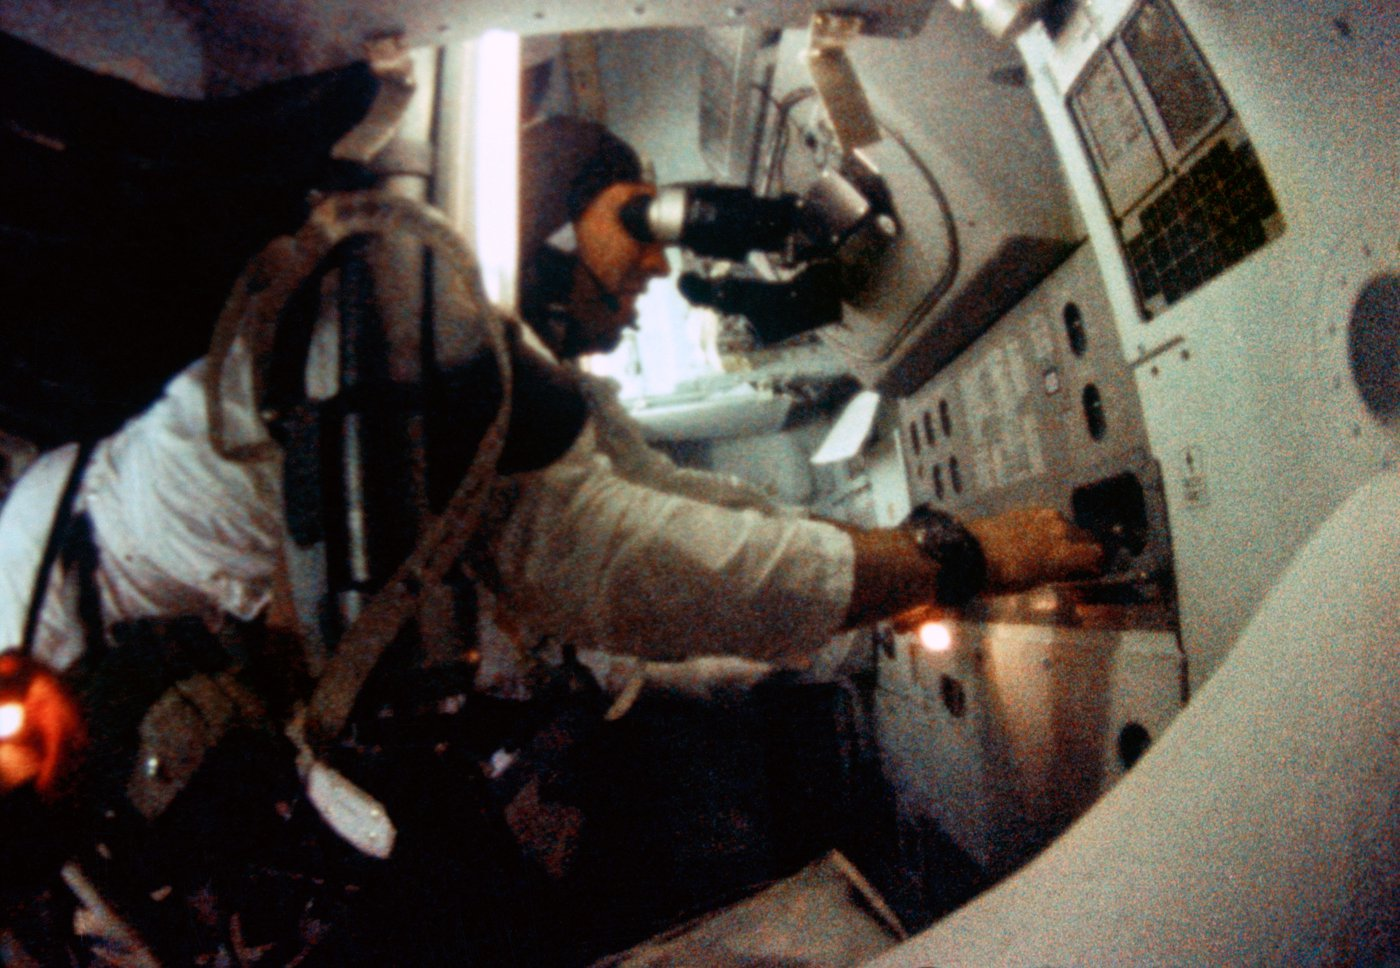
\includegraphics[height=0.21\textheight]{ch10_apollo8_navigation_1968.jpg}\\[1mm]
\imgcap{Apollo 8 (1968): Jim Lovell la stația de ghidare și navigație}
\imgcredit{https://commons.wikimedia.org/wiki/File:Apollo_8_Lovell_at_Guidance_and_Navigation_station.jpg}{Foto: NASA (1968); domeniu public; Wikimedia Commons}
\end{column}
\begin{column}{0.58\textwidth}
\begin{itemize}
    \item \refKalman: o estimare recursivă a unei stări ascunse din măsurători zgomotoase
    \begin{itemize}
        \item la fiecare pas: prezicem starea, apoi corectăm predicția cu noua măsurătoare
        \item ponderea corecției, \textbf{cîștigul Kalman}, echilibrează cele două surse de incertitudine
    \end{itemize}
    \item Filtrul a fost adaptat la NASA Ames pentru navigația navelor Apollo
    \begin{itemize}
        \item starea: poziția și viteza; măsurătorile: observații ale stelelor și radar
    \end{itemize}
    \item În economie starea este un trend, un ciclu, un coeficient sau un regim; măsurătorile sînt datele publicate
\end{itemize}
\end{column}
\end{columns}
\end{frame}

\begin{frame}{Stări ascunse în economie și finanțe}
\itemsize{\small}
\begin{center}
\footnotesize
\begin{tabular}{>{\raggedright\arraybackslash}p{3.6cm}>{\raggedright\arraybackslash}p{3.6cm}>{\raggedright\arraybackslash}p{3.4cm}}
\toprule
\textbf{Seria observată} & \textbf{Starea ascunsă} & \textbf{Modelul din acest capitol} \\
\midrule
Debitul Nilului, inflația lunară & nivelul de fond & local level \\
PIB real & trendul și deviația PIB & componente neobservate \\
randamentele unui indice bursier & un beta variabil în timp & regresie cu parametri variabili \\
mai mulți indicatori de activitate & un factor comun & model cu factori dinamici \\
creșterea PIB, randamentele & recesiune sau expansiune; calm sau agitat & Markov switching \\
\bottomrule
\end{tabular}
\end{center}
\begin{itemize}
    \item Primele patru au o stare \textbf{continuă} și sînt filtrate cu filtrul Kalman
    \item Ultimul are o stare \textbf{discretă} (un regim) și este filtrat cu filtrul Hamilton
    \item Ambele filtre fac același lucru: prezic starea, apoi actualizează predicția cu $y_t$
\end{itemize}
\end{frame}


%=============================================================================
\section{Forma în spațiul stărilor}
%=============================================================================

\begin{frame}{Forma în spațiul stărilor}
\itemsize{\small}
\begin{itemize}
    \item \textbf{Ecuația de măsurare}: $y_t = Z_t\alpha_t + \varepsilon_t$, \quad $\varepsilon_t \sim N(0, H)$
    \begin{itemize}
        \item $y_t$: observația (aici un scalar); $\alpha_t$: \textbf{vectorul de stare} ($m \times 1$), neobservat; $Z_t$: un rînd $1 \times m$ de numere cunoscute
    \end{itemize}
    \item \textbf{Ecuația de tranziție}: $\alpha_{t+1} = T\alpha_t + R\eta_t$, \quad $\eta_t \sim N(0, Q)$
    \begin{itemize}
        \item starea evoluează ca o autoregresie vectorială de ordinul 1 (VAR(1), \tsachlink{https://danpele.github.io/Time-Series-Analysis/RO/Cursuri/capitol6_modele_var_cauzalitate_granger.pdf}{Capitolul 6}); $T$ este $m \times m$
        \item $R$: transmite șocurile $\eta_t$ în stare; $H$, $Q$: varianțele șocurilor de măsurare și ale șocurilor stării
        \item starea inițială: $\alpha_1 \sim N(a_1, P_1)$, $a_1$, $P_1$: media și varianța ei; $\varepsilon_t$, $\eta_s$ și $\alpha_1$ sînt independente între ele
    \end{itemize}
    \item \textbf{Matricele sistemului} $Z_t, H, T, R, Q$ conțin parametrii $\theta$; aceștia se estimează prin verosimilitate maximă
    \begin{itemize}
        \item aceeași formă acoperă ARMA, netezirea exponențială, modelele trend--ciclu, regresiile cu coeficienți mobili și modelele factoriale \refDK
    \end{itemize}
\end{itemize}
\end{frame}

\begin{frame}{Modelul local level}
\itemsize{\small}
\begin{itemize}
    \item \textbf{Local level} (mers aleator plus zgomot): $y_t = \mu_t + \varepsilon_t$, \quad $\mu_{t+1} = \mu_t + \eta_t$
    \begin{itemize}
        \item starea $\alpha_t = \mu_t$, nivelul; $Z = T = R = 1$, $H = \sigma^2_\varepsilon$, $Q = \sigma^2_\eta$
        \item $\varepsilon_t$: zgomot de măsurare care dispare în perioada următoare; $\eta_t$: o deplasare permanentă a nivelului
    \end{itemize}
    \item \textbf{Raportul semnal--zgomot} $q = \sigma^2_\eta/\sigma^2_\varepsilon$: cîtă parte din mișcare este permanentă
    \begin{itemize}
        \item $q = 0$: un nivel constant (zgomot alb în jurul unei medii); $q \to \infty$: un mers aleator pur
    \end{itemize}
    \item Forma redusă: $\Delta y_t = \eta_{t-1} + \varepsilon_t - \varepsilon_{t-1}$ este un MA(1) cu $\rho(1) = -1/(q+2)$
    \begin{itemize}
        \item deci modelul local level este un ARIMA(0,1,1) (\tsachlink{https://danpele.github.io/Time-Series-Analysis/RO/Cursuri/capitol3_radacini_unitare_modele_arima.pdf}{Capitolul 3}) cu un coeficient MA negativ
        \item $\gamma(0) = \sigma^2_\eta + 2\sigma^2_\varepsilon$ și $\gamma(1) = -\sigma^2_\varepsilon$ dau $\rho(1)$
    \end{itemize}
\end{itemize}
\end{frame}

\begin{frame}{Traiectorii local level și local linear trend}
\itemsize{\footnotesize}
\begin{center}
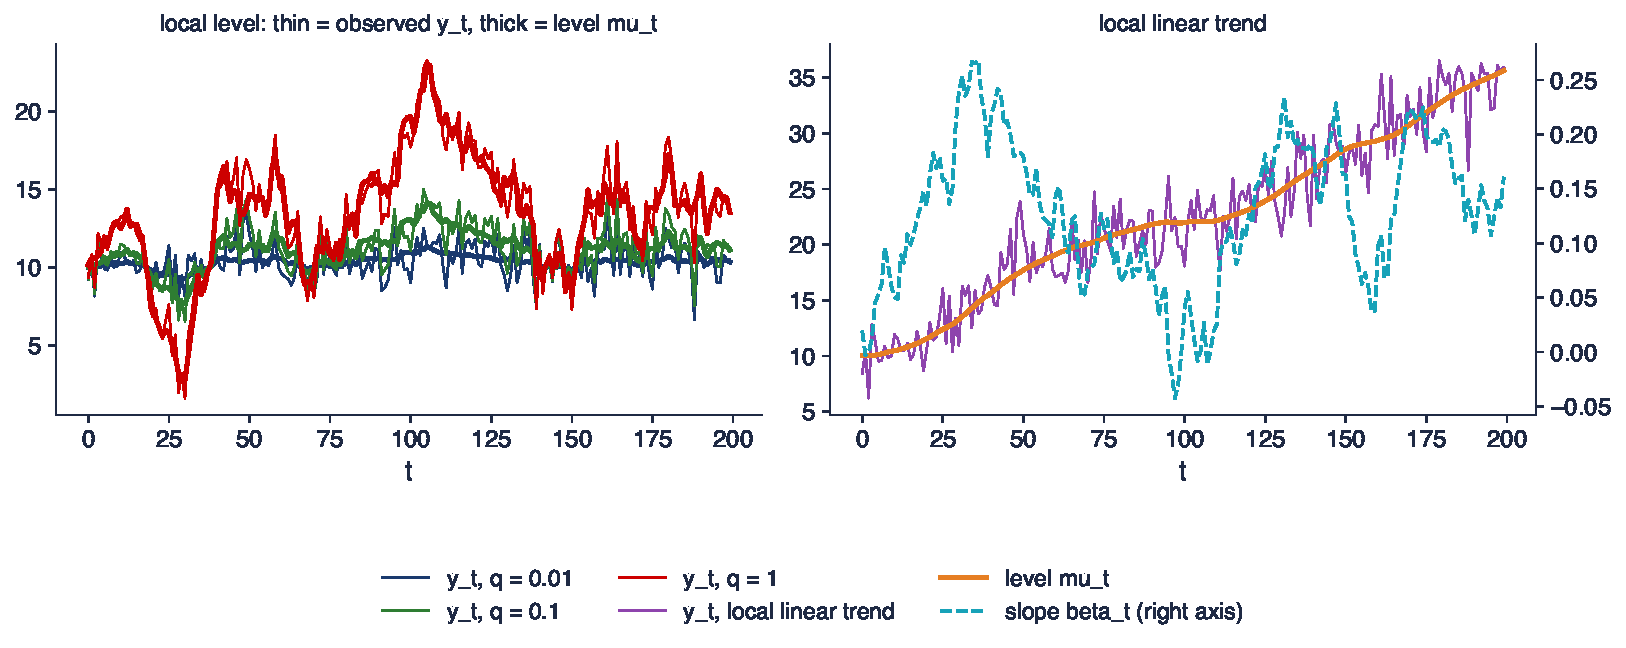
\includegraphics[width=0.97\textwidth,height=0.66\textheight,keepaspectratio]{tsa_ch10_ss_examples.pdf}
\end{center}
\vspace{-0.25cm}
\begin{itemize}
    \item Stînga: aceleași șocuri $\varepsilon_t, \eta_t \sim N(0, 1)$, cu $\sigma^2_\varepsilon = 1$ și $q = 0{,}01;\ 0{,}1;\ 1$ (subțire: $y_t$, gros: $\mu_t$). Dreapta: un local linear trend, a cărui pantă $\beta_t$ este ea însăși un mers aleator
\end{itemize}
\quantlet{TSA\_ch10\_state\_space\_examples}{\qlurl{TSA_ch10_state_space_examples}}
\end{frame}

\begin{frame}{Interpretarea traiectoriilor simulate}
\itemsize{\small}
\begin{itemize}
    \item $q$ mic: nivelul abia se mișcă, iar $y_t$ arată ca un zgomot în jurul unei medii; $q$ mare: nivelul rătăcește, iar $y_t$ îl urmează
    \begin{itemize}
        \item autocorelația primei diferențe: \ensuremath{-}0{,}51 pentru $q = 0{,}01$ (teoretic $-1/2{,}01$) și \ensuremath{-}0{,}28 pentru $q = 1$ (teoretic $-1/3$)
    \end{itemize}
    \item Local linear trend are o pantă care se schimbă lent: perioade de creștere rapidă și lentă
    \begin{itemize}
        \item acesta este modelul de trend pe care îl vom folosi pentru PIB
    \end{itemize}
    \item Problema de estimare: doar din $y_t$, cît este nivel și cît este zgomot? Filtrul Kalman răspunde pentru varianțe date; verosimilitatea alege varianțele
\end{itemize}
\end{frame}

\begin{frame}{Modelul local linear trend}
\itemsize{\small}
\begin{itemize}
    \item \textbf{Local linear trend}: $y_t = \mu_t + \varepsilon_t$, \quad $\mu_{t+1} = \mu_t + \beta_t + \eta_t$, \quad $\beta_{t+1} = \beta_t + \zeta_t$
    \begin{itemize}
        \item starea $\alpha_t = (\mu_t, \beta_t)'$: nivelul și panta (rata de creștere)
        \item $Z = (1,\ 0)$, \quad $T = \begin{pmatrix}1 & 1\\ 0 & 1\end{pmatrix}$, \quad $Q = \mathrm{diag}(\sigma^2_\eta, \sigma^2_\zeta)$
    \end{itemize}
    \item Cazuri particulare
    \begin{itemize}
        \item $\sigma^2_\eta = \sigma^2_\zeta = 0$: un trend liniar determinist $\mu_1 + \beta_1 t$ (\tsachlink{https://danpele.github.io/Time-Series-Analysis/RO/Cursuri/capitol3_radacini_unitare_modele_arima.pdf}{Capitolul 3})
        \item $\sigma^2_\zeta = 0$: un mers aleator cu deriva $\beta$
        \item $\sigma^2_\eta = 0$: \textbf{trendul neted} (mers aleator integrat), modelul din spatele filtrului HP (secțiunea 5)
    \end{itemize}
    \item Prognozele: $\hat y_{T+h} = \hat\mu_T + h\hat\beta_T$, versiunea în spațiul stărilor a metodei Holt (\tsachlink{https://danpele.github.io/Time-Series-Analysis/RO/Cursuri/capitol0_introducere.pdf}{Capitolul 0})
\end{itemize}
\end{frame}

\begin{frame}{Modele ARMA în forma în spațiul stărilor}
\itemsize{\small}
\begin{itemize}
    \item \textbf{AR(2)}: $y_t = \phi_1y_{t-1} + \phi_2y_{t-2} + u_t$; starea $\alpha_t = (y_t, y_{t-1})'$
    \begin{itemize}
        \item $y_t = (1,\ 0)\,\alpha_t$ ($H = 0$), \quad $\alpha_{t+1} = \begin{pmatrix}\phi_1 & \phi_2\\ 1 & 0\end{pmatrix}\alpha_t + \begin{pmatrix}1\\ 0\end{pmatrix}u_{t+1}$
        \item $T$ este matricea companion din \tsachlink{https://danpele.github.io/Time-Series-Analysis/RO/Cursuri/capitol2_modele_arma.pdf}{Capitolul 2}; valorile ei proprii sînt inversele rădăcinilor AR
    \end{itemize}
    \item \textbf{ARMA(1,1)}: $y_t = \phi y_{t-1} + u_t + \theta u_{t-1}$, cu $\alpha_t = (y_t, \theta u_t)'$
    \begin{itemize}
        \item $T = \begin{pmatrix}\phi & 1\\ 0 & 0\end{pmatrix}$, $R = (1,\ \theta)'$; orice ARMA$(p,q)$ se scrie cu $m = \max(p, q+1)$
    \end{itemize}
    \item Importanța practică: filtrul Kalman dă verosimilitatea gaussiană \textbf{exactă} a unui model ARMA, chiar cu valori lipsă
    \begin{itemize}
        \item pornirea staționară: $P_1$ rezolvă $P = TPT' + RQR'$, adică $\mathrm{vec}(P_1) = (I - T \otimes T)^{-1}\mathrm{vec}(RQR')$
        \item așa estimează \texttt{statsmodels} \texttt{SARIMAX} modelele ARIMA din \tsachlink{https://danpele.github.io/Time-Series-Analysis/RO/Cursuri/capitol2_modele_arma.pdf}{Capitolele 2}--\tsachlink{https://danpele.github.io/Time-Series-Analysis/RO/Cursuri/capitol4_sezonalitate_prognoza.pdf}{4}
    \end{itemize}
\end{itemize}
\end{frame}

\begin{frame}{Exemplu rezolvat: AR(2) pentru creșterea PIB din SUA}
\itemsize{\small}
\begin{itemize}
    \item Date: creșterea PIB real al SUA, trimestru față de trimestru, 1947--2019 ($T = 291$, FRED GDPC1)
    \begin{itemize}
        \item AR(2) cu termen liber estimat cu \texttt{SARIMAX}: $\hat\phi_1 = 0{,}319$, $\hat\phi_2 = 0{,}111$, $\hat\sigma^2 = 0{,}739$, media $\hat\mu = 0{,}774\%$ pe trimestru
    \end{itemize}
    \item Filtrul nostru, cu matricele din slide-ul anterior și cu $P_1$ staționar
    \begin{itemize}
        \item log-verosimilitatea: Kalman \ensuremath{-}368{,}9157; \texttt{SARIMAX} \ensuremath{-}368{,}9157: același număr
    \end{itemize}
    \item Erorile de predicție $v_t$ ale filtrului sînt erorile de prognoză la un pas ale AR(2); verosimilitatea se construiește din ele (secțiunea 4)
\end{itemize}
\end{frame}

\begin{frame}{Regresie cu parametri variabili în timp}
\itemsize{\small}
\begin{itemize}
    \item \textbf{Regresia cu parametri variabili în timp} (TVP): $y_t = \alpha + \beta_t x_t + \varepsilon_t$, \quad $\beta_{t+1} = \beta_t + \eta_t$
    \begin{itemize}
        \item starea $(\alpha, \beta_t)'$; rîndul $Z_t = (1,\ x_t)$ \textbf{se schimbă în timp}; $Q = \mathrm{diag}(0, \sigma^2_\eta)$
        \item $\sigma^2_\eta = 0$: metoda celor mai mici pătrate (OLS), calculată recursiv
    \end{itemize}
    \item Exemple
    \begin{itemize}
        \item un beta de piață care crește în crize; transmiterea cursului de schimb în inflație; persistența inflației
    \end{itemize}
    \item Mai bună decît o fereastră mobilă: nu alegem lungimea ferestrei, folosim toate observațiile, iar $\beta_t$ vine cu o eroare standard
\end{itemize}
\end{frame}

\begin{frame}{Netezirea exponențială ca model în spațiul stărilor}
\itemsize{\small}
\begin{itemize}
    \item \tsachlink{https://danpele.github.io/Time-Series-Analysis/RO/Cursuri/capitol0_introducere.pdf}{Capitolul 0}: netezirea exponențială simplă (SES) actualizează un nivel $\ell_t = \alpha y_t + (1-\alpha)\ell_{t-1}$ și prognozează $\hat y_{t+1} = \ell_t$
    \begin{itemize}
        \item echivalent $\ell_t = \ell_{t-1} + \alpha(y_t - \ell_{t-1})$: nivelul vechi plus o fracțiune $\alpha$ din surpriză
    \end{itemize}
    \item \refMuth: SES dă prognozele optime atunci cînd datele urmează modelul local level
    \begin{itemize}
        \item secțiunea 3 o arată: $\alpha$ este cîștigul Kalman de echilibru
    \end{itemize}
    \item Modelele ETS (eroare, trend, sezonalitate) sînt modele în spațiul stărilor cu o singură sursă de eroare \refHKOS; modelele de aici au șocuri separate pentru fiecare componentă
\end{itemize}
\end{frame}

\begin{frame}{Recapitulare: forma în spațiul stărilor}
\itemsize{\small}
\begin{itemize}
    \item $y_t = Z_t\alpha_t + \varepsilon_t$, $\alpha_{t+1} = T\alpha_t + R\eta_t$: un VAR(1) ascuns, observat cu zgomot
    \item Local level: $q = \sigma^2_\eta/\sigma^2_\varepsilon$; forma redusă ARIMA(0,1,1)
    \item Local linear trend, ARMA și regresia TVP sînt alte alegeri ale lui $Z_t, T, Q$
    \item Verosimilitatea Kalman a unui AR(2) este egală cu verosimilitatea ARMA exactă
\end{itemize}
\end{frame}


%=============================================================================
\section{Filtrul Kalman}
%=============================================================================

\begin{frame}{Ideea filtrului}
\itemsize{\small}
\begin{itemize}
    \item Notație: $Y_t = (y_1, \dots, y_t)$; urmărim două mărimi (vectori) pentru stare
    \begin{itemize}
        \item predicția: $a_t = E(\alpha_t \mid Y_{t-1})$, cu varianța $P_t$
        \item estimarea filtrată: $a_{t|t} = E(\alpha_t \mid Y_t)$, cu varianța $P_{t|t}$
    \end{itemize}
    \item Fiecare perioadă are doi pași
    \begin{itemize}
        \item \textbf{actualizarea}: sosește $y_t$; corectăm $a_t$ cu o fracțiune din surpriza $v_t = y_t - Z_ta_t$
        \item \textbf{predicția}: trecem starea filtrată prin ecuația de tranziție și obținem $a_{t+1}$
    \end{itemize}
    \item Cu erori gaussiene, $a_{t|t}$ este media condiționată exactă; fără normalitate rămîne cea mai bună estimare \textbf{liniară} \refDK
    \item Pornirea: $a_1, P_1$; pentru o stare nestaționară folosim o pornire \textbf{difuză} ($P_1$ foarte mare: nu știm nimic)
\end{itemize}
\end{frame}

\begin{frame}{Cei doi pași în formule}
\itemsize{\small}
\begin{itemize}
    \item \textbf{Actualizarea} (cînd $y_t$ este observat)
    \begin{itemize}
        \item eroarea de predicție $v_t = y_t - Z_ta_t$, cu varianța $F_t = Z_tP_tZ_t' + H$
        \item \textbf{cîștigul Kalman} $K_t = P_tZ_t'F_t^{-1}$
        \item $a_{t|t} = a_t + K_tv_t$, \quad $P_{t|t} = P_t - K_tZ_tP_t$
    \end{itemize}
    \item \textbf{Predicția}
    \begin{itemize}
        \item $a_{t+1} = Ta_{t|t}$, \quad $P_{t+1} = TP_{t|t}T' + RQR'$
    \end{itemize}
    \item \textbf{Local level}: $F_t = P_t + \sigma^2_\varepsilon$, \quad $K_t = P_t/(P_t + \sigma^2_\varepsilon)$
    \begin{itemize}
        \item $a_{t+1} = a_t + K_t(y_t - a_t)$, \quad $P_{t+1} = P_t(1 - K_t) + \sigma^2_\eta$
    \end{itemize}
    \item Lipsește $y_t$: sărim peste actualizare ($a_{t|t} = a_t$, $P_{t|t} = P_t$) și facem predicția
\end{itemize}
\end{frame}

\begin{frame}{Cîștigul Kalman}
\itemsize{\small}
\begin{itemize}
    \item Local level: $K_t = \dfrac{P_t}{P_t + \sigma^2_\varepsilon}$ este ponderea noii observații, între 0 și 1
    \begin{itemize}
        \item $a_{t|t} = (1 - K_t)\,a_t + K_t\,y_t$: o medie ponderată a predicției și a observației
    \end{itemize}
    \item Două incertitudini concurează
    \begin{itemize}
        \item măsurători zgomotoase ($\sigma^2_\varepsilon$ mare): $K_t$ mic, avem încredere în model
        \item stare incertă ($P_t$ mare, de exemplu la început sau după valori lipsă): $K_t$ mare, avem încredere în date
    \end{itemize}
    \item Varianța scade întotdeauna după o observație: $P_{t|t} = (1 - K_t)P_t \le P_t$
    \begin{itemize}
        \item și crește cu $\sigma^2_\eta$ în pasul de predicție: cele două forțe se echilibrează într-o stare de echilibru
    \end{itemize}
    \item Aceeași formulă ca la ponderarea a două estimări independente după precizia lor, $1/P_t$ și $1/\sigma^2_\varepsilon$
\end{itemize}
\end{frame}

\begin{frame}{Exemplu rezolvat: trei perioade de mînă (1/2)}
\itemsize{\small}
\begin{itemize}
    \item Local level cu $\sigma^2_\varepsilon = 4$, $\sigma^2_\eta = 1$ ($q = 0{,}25$); a priori $a_1 = 10$, $P_1 = 4$; datele $y = (12, 11, 14)$
    \begin{itemize}
        \item $t = 1$: $F_1 = 4 + 4 = 8$, $K_1 = 4/8 = 0{,}5$, $v_1 = 12 - 10 = 2$
        \item $a_{1|1} = 10 + 0{,}5 \cdot 2 = 11$, $P_{1|1} = 4(1 - 0{,}5) = 2$; predicția $a_2 = 11$, $P_2 = 2 + 1 = 3$
    \end{itemize}
    \item $t = 2$: $F_2 = 3 + 4 = 7$, $K_2 = 3/7 = 0{,}429$, $v_2 = 11 - 11 = 0$
    \begin{itemize}
        \item nicio surpriză: nivelul rămîne $a_{2|2} = 11$, dar incertitudinea scade la $P_{2|2} = 3 \cdot 4/7 = 1{,}71$
        \item predicția $a_3 = 11$, $P_3 = 1{,}71 + 1 = 2{,}71$
    \end{itemize}
    \item Cîștigul scade de la 0,5 la 0{,}429: filtrul învață despre nivel și se bazează mai puțin pe fiecare observație nouă
\end{itemize}
\end{frame}

\begin{frame}{Exemplu rezolvat: trei perioade de mînă (2/2)}
\itemsize{\small}
\begin{center}
\footnotesize
\begin{tabular}{ccccccccc}
\toprule
$t$ & $y_t$ & $a_t$ & $P_t$ & $F_t$ & $K_t$ & $v_t$ & $a_{t|t}$ & $P_{t|t}$ \\
\midrule
1 & 12 & 10{,}00 & 4{,}00 & 8{,}00 & 0{,}500 & 2 & 11{,}00 & 2{,}00 \\
2 & 11 & 11{,}00 & 3{,}00 & 7{,}00 & 0{,}429 & 0 & 11{,}00 & 1{,}71 \\
3 & 14 & 11{,}00 & 2{,}71 & 6{,}71 & 0{,}404 & 3 & 12{,}21 & 1{,}62 \\
\bottomrule
\end{tabular}
\end{center}
\begin{itemize}
    \item $t = 3$: $K_3 = 2{,}71/6{,}71 = 0{,}404$, $v_3 = 14 - 11 = 3$, $a_{3|3} = 11 + 0{,}404 \cdot 3 = 12{,}21$
    \begin{itemize}
        \item prognoza pentru $t = 4$: $a_4 = 12{,}21$, cu $P_4 = 2{,}62$; prognoza lui $y_4$ are varianța $P_4 + \sigma^2_\varepsilon$
    \end{itemize}
    \item Cîștigul continuă să scadă spre starea de echilibru $\bar K = 0{,}390$ ($\bar P = 2{,}56$, slide-ul următor)
    \begin{itemize}
        \item surpriza de 3 mută nivelul doar cu $0{,}404 \cdot 3$: o parte din ea este tratată ca zgomot
    \end{itemize}
\end{itemize}
\end{frame}

\begin{frame}{Starea de echilibru și netezirea exponențială}
\itemsize{\small}
\begin{itemize}
    \item Pentru modelul local level, $P_t$ converge la soluția ecuației $\bar P = \bar P(1 - \bar K) + \sigma^2_\eta$, cu $\bar K = \bar P/(\bar P + \sigma^2_\varepsilon)$
    \begin{itemize}
        \item soluția: $\bar P = \sigma^2_\varepsilon\,\dfrac{q + \sqrt{q^2 + 4q}}{2}$, \quad $\bar K = \dfrac{\bar P}{\bar P + \sigma^2_\varepsilon}$
        \item exemplu: $q = 0{,}25$ dă $\bar P/\sigma^2_\varepsilon = (0{,}25 + \sqrt{1{,}0625})/2 = 2{,}56/4$ și $\bar K = 0{,}390$
    \end{itemize}
    \item În starea de echilibru: $a_{t+1} = a_t + \bar K(y_t - a_t) = \bar K y_t + (1 - \bar K)a_t$
    \begin{itemize}
        \item aceasta este SES cu $\alpha = \bar K$: netezirea exponențială este filtrul Kalman al unui model local level \refMuth
    \end{itemize}
    \item Relația inversă: o pondere SES $\alpha$ corespunde lui $q = \alpha^2/(1 - \alpha)$
    \begin{itemize}
        \item versiunea în spațiul stărilor adaugă ce îi lipsește SES: o verosimilitate pentru $q$, intervale de prognoză, valori lipsă
    \end{itemize}
\end{itemize}
\end{frame}

\begin{frame}{Nilul: filtrul Kalman pentru modelul local level}
\itemsize{\footnotesize}
\begin{center}
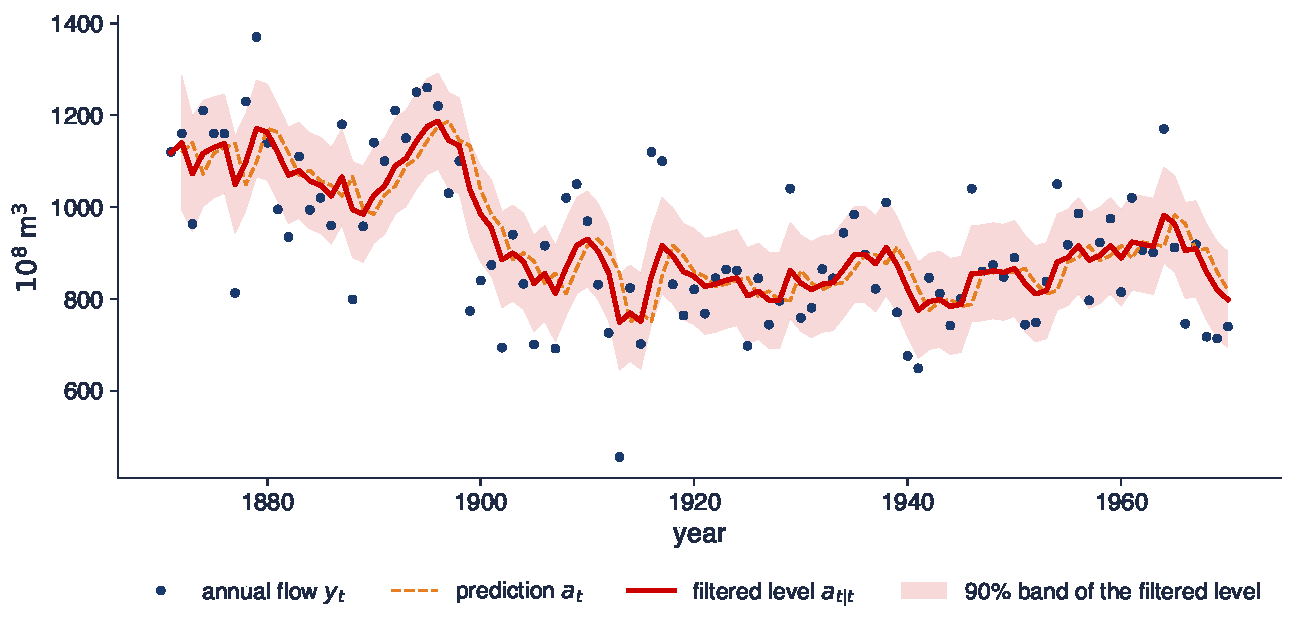
\includegraphics[width=0.97\textwidth,height=0.58\textheight,keepaspectratio]{tsa_ch10_nile_filter.pdf}
\end{center}
\vspace{-0.25cm}
\begin{itemize}
    \item Debitul anual la Aswan, 1871--1970 ($10^8$ m$^3$, statsmodels); varianțele prin verosimilitate maximă, cu pornire difuză: $\hat\sigma^2_\varepsilon = 15100$, $\hat\sigma^2_\eta = 1468$, $\hat q = 0{,}097$, estimările din \refDK
\end{itemize}
\quantlet{TSA\_ch10\_kalman\_filter}{\qlurl{TSA_ch10_kalman_filter}}
\end{frame}

\begin{frame}{Interpretarea filtrului pentru Nil}
\itemsize{\small}
\begin{itemize}
    \item Cea mai mare parte a mișcării de la un an la altul este zgomot: $\hat q = 0{,}097$, deci fiecare debit mută nivelul cu aproximativ un sfert din surpriză ($\bar K = 0{,}267$)
    \begin{itemize}
        \item \texttt{statsmodels} \texttt{UnobservedComponents('llevel')} dă 15078 și 1479: același model, o pornire puțin diferită
    \end{itemize}
    \item 1899: debitul este 774, nivelul prezis 1133; surpriza $v = \ensuremath{-}359$ coboară nivelul doar la 1037
    \begin{itemize}
        \item filtrul are nevoie de mai mulți ani slabi pentru a accepta noul nivel (834 în 1905): primul baraj de la Aswan a fost finalizat în 1902
    \end{itemize}
    \item În 1970 nivelul este 798, cu eroarea standard 63, mult sub media eșantionului, 919
\end{itemize}
\end{frame}

\begin{frame}{Cîștigul converge; SES reproduce filtrul}
\itemsize{\footnotesize}
\begin{center}
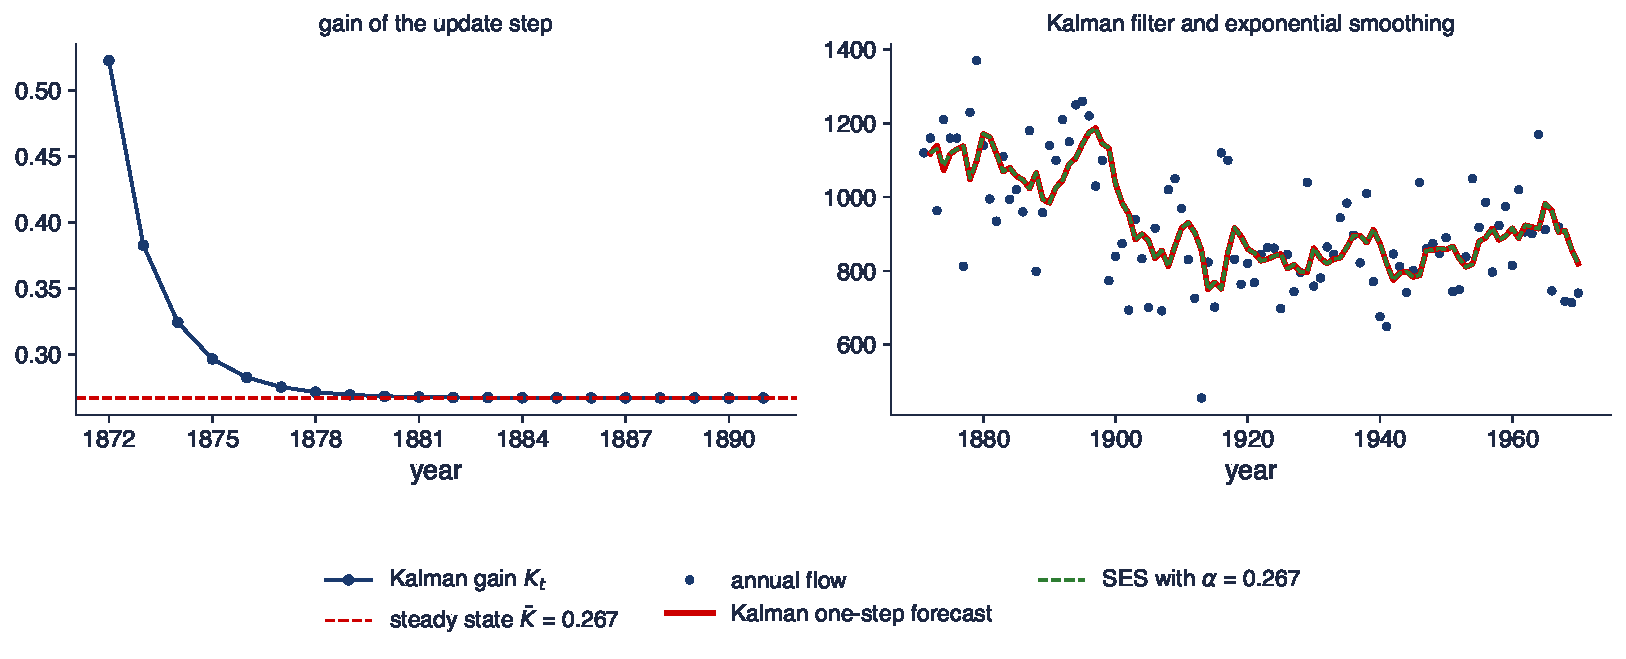
\includegraphics[width=0.97\textwidth,height=0.66\textheight,keepaspectratio]{tsa_ch10_gain_ses.pdf}
\end{center}
\vspace{-0.25cm}
\begin{itemize}
    \item Stînga: $K_t$ al filtrului pentru Nil; dreapta: prognozele Kalman la un pas $a_{t}$ și SES cu $\alpha = \bar K$, pornită de la prima observație
\end{itemize}
\quantlet{TSA\_ch10\_kalman\_filter}{\qlurl{TSA_ch10_kalman_filter}}
\end{frame}

\begin{frame}{Interpretarea cîștigului}
\itemsize{\small}
\begin{itemize}
    \item $K_t$ pornește de la 0{,}523 (după pornirea difuză), 0{,}297 în anul 5 și ajunge la mai puțin de 0,001 de $\bar K = 0{,}267$ după 10 ani
    \begin{itemize}
        \item prognozele diferă cu 0{,}24 în anul 5 și cu mai puțin de 0{,}02 după 20 de ani
    \end{itemize}
    \item SES estimată direct prin cele mai mici pătrate (\tsachlink{https://danpele.github.io/Time-Series-Analysis/RO/Cursuri/capitol0_introducere.pdf}{Capitolul 0}) dă $\hat\alpha = 0{,}246$, adică $q = \alpha^2/(1-\alpha) = 0{,}080$
    \begin{itemize}
        \item aproape de răspunsul verosimilității: două criterii, un singur model
    \end{itemize}
    \item Perspectiva spațiului stărilor explică SES: $\alpha$ este mare cînd nivelul se mișcă mult în raport cu zgomotul
\end{itemize}
\end{frame}

\begin{frame}{Recapitulare: filtrul Kalman}
\itemsize{\small}
\begin{itemize}
    \item Actualizarea: $v_t = y_t - Z_ta_t$, $F_t = Z_tP_tZ_t' + H$, $K_t = P_tZ_t'F_t^{-1}$, $a_{t|t} = a_t + K_tv_t$
    \item Predicția: $a_{t+1} = Ta_{t|t}$, $P_{t+1} = TP_{t|t}T' + RQR'$
    \item Cîștigul cîntărește datele în raport cu modelul; se stabilizează într-o stare de echilibru
    \item Local level în starea de echilibru = SES cu $\alpha = \bar K$; Nilul: $\bar K = 0{,}267$
\end{itemize}
\end{frame}


%=============================================================================
\section{Netezire, verosimilitate și valori lipsă}
%=============================================================================

\begin{frame}{Netezirea: folosim tot eșantionul}
\itemsize{\small}
\begin{itemize}
    \item \textbf{Filtrarea} folosește $Y_t$ (trecutul și prezentul): estimarea în timp real
    \begin{itemize}
        \item \textbf{netezirea} folosește $Y_n$ (tot eșantionul): $\hat\alpha_t = E(\alpha_t \mid Y_n)$, cu varianța $V_t \le P_{t|t}$
    \end{itemize}
    \item Netezitorul \textbf{Rauch--Tung--Striebel} \refRTS: o trecere înapoi după filtru, de la $t = n-1$ la 1
    \begin{itemize}
        \item $n$: volumul eșantionului; $J_t$: cîștigul netezitorului, ponderea revizuirii care vine din viitor
        \item $J_t = P_{t|t}T'P_{t+1}^{-1}$, \quad $\hat\alpha_t = a_{t|t} + J_t(\hat\alpha_{t+1} - a_{t+1})$
        \item $V_t = P_{t|t} + J_t(V_{t+1} - P_{t+1})J_t'$; la $t = n$ estimarea netezită și cea filtrată coincid
    \end{itemize}
    \item Utilizare: starea filtrată pentru decizii în timp real și prognoză; starea netezită pentru istorie (datarea rupturilor, deviația PIB din trecut)
\end{itemize}
\end{frame}

\begin{frame}{Nilul: nivelul filtrat și nivelul netezit}
\itemsize{\footnotesize}
\begin{center}
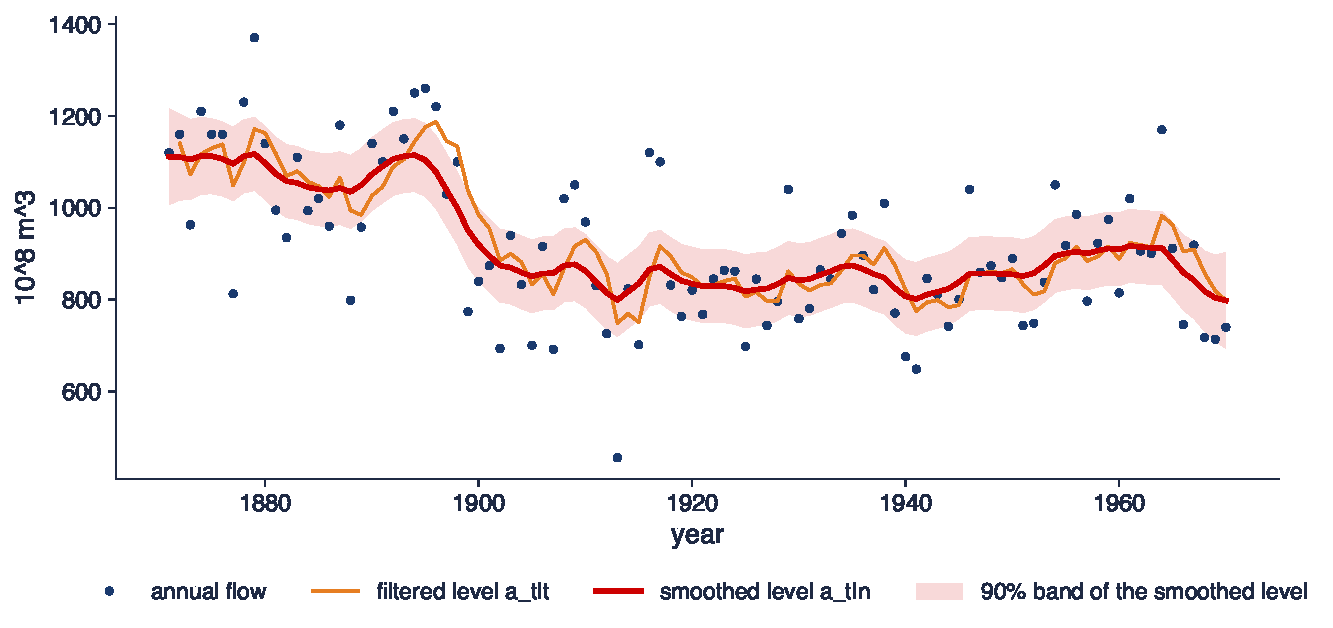
\includegraphics[width=0.97\textwidth,height=0.58\textheight,keepaspectratio]{tsa_ch10_nile_smooth.pdf}
\end{center}
\vspace{-0.25cm}
\begin{itemize}
    \item Nivelul filtrat $a_{t|t}$ și nivelul netezit $\hat\alpha_t$, cu banda de 90\%; aceleași varianțe de verosimilitate maximă
\end{itemize}
\quantlet{TSA\_ch10\_smoothing\_likelihood}{\qlurl{TSA_ch10_smoothing_likelihood}}
\end{frame}

\begin{frame}{Interpretarea nivelului netezit}
\itemsize{\small}
\begin{itemize}
    \item Nivelul netezit reacționează la scăderea din 1898--1899 \textbf{înainte} ca ea să apară în date: în 1897 este deja 1038, față de 1145 filtrat
    \begin{itemize}
        \item folosește informație din viitor: util pentru istorie, imposibil în timp real
    \end{itemize}
    \item În 1900: netezit 920, filtrat 985; nivelul netezit se adaptează mai repede, pentru că vede anii slabi de după 1900
    \begin{itemize}
        \item eroarea standard în 1920: 48 netezit, față de 63 filtrat
    \end{itemize}
    \item Traiectoria netezită arată o treaptă în jurul anului 1899 mai clar decît orice medie mobilă din \tsachlink{https://danpele.github.io/Time-Series-Analysis/RO/Cursuri/capitol0_introducere.pdf}{Capitolul 0}
\end{itemize}
\end{frame}

\begin{frame}{Verosimilitatea: descompunerea erorilor de predicție}
\itemsize{\small}
\begin{itemize}
    \item Densitatea comună se descompune în densități condiționate la un pas: $p(y_1, \dots, y_n) = \prod_t p(y_t \mid Y_{t-1})$
    \begin{itemize}
        \item cu erori gaussiene, $y_t \mid Y_{t-1} \sim N(Z_ta_t, F_t)$: filtrul dă media și varianța
    \end{itemize}
    \item \textbf{Descompunerea erorilor de predicție}
    \begin{itemize}
        \item $\log L(\theta) = -\dfrac{n}{2}\log 2\pi - \dfrac12\sum_{t=1}^{n}\left(\log F_t + \dfrac{v_t^2}{F_t}\right)$
        \item $\theta$: parametrii (varianțele modelului); $v_t$, $F_t$: erorile de predicție și varianțele lor, date de filtru
        \item o rulare a filtrului dă $\log L$ pentru o valoare a lui $\theta$; un optimizator numeric caută după $\theta$
    \end{itemize}
    \item Pornirea difuză: primii $d$ termeni (aici $d = 1$ pentru nivel) sînt omiși, deoarece acolo $F_t$ este uriaș \refDK
    \item Aceeași idee ca verosimilitatea ARMA exactă din \tsachlink{https://danpele.github.io/Time-Series-Analysis/RO/Cursuri/capitol2_modele_arma.pdf}{Capitolul 2}, acum pentru orice model în spațiul stărilor
\end{itemize}
\end{frame}

\begin{frame}{Verosimilitatea maximă în practică}
\itemsize{\small}
\begin{itemize}
    \item Optimizăm după $\log\sigma^2$ (varianțele rămîn pozitive); mai multe valori de pornire, deoarece suprafața poate fi plată
    \begin{itemize}
        \item o varianță estimată la zero este frecventă și are sens: acea componentă este deterministă
    \end{itemize}
    \item \textbf{Concentrarea}: pentru local level scriem $\sigma^2_\eta = q\sigma^2_\varepsilon$; pentru $q$ fixat, $\hat\sigma^2_\varepsilon = \frac{1}{n-1}\sum_t v_t^2/F_t$ are formă închisă
    \begin{itemize}
        \item log-verosimilitatea profil devine atunci o funcție doar de $q$ (graficul următor)
    \end{itemize}
    \item Erorile standard din hessiana numerică; alegerea modelului după AIC și BIC; teste pe erorile de predicție standardizate $e_t = v_t/\sqrt{F_t}$
    \begin{itemize}
        \item \texttt{statsmodels}: \texttt{UnobservedComponents}, \texttt{SARIMAX}, \texttt{DynamicFactor} folosesc toate acest mecanism
    \end{itemize}
\end{itemize}
\end{frame}

\begin{frame}{Verosimilitatea profil și alegerea lui $q$}
\itemsize{\footnotesize}
\begin{center}
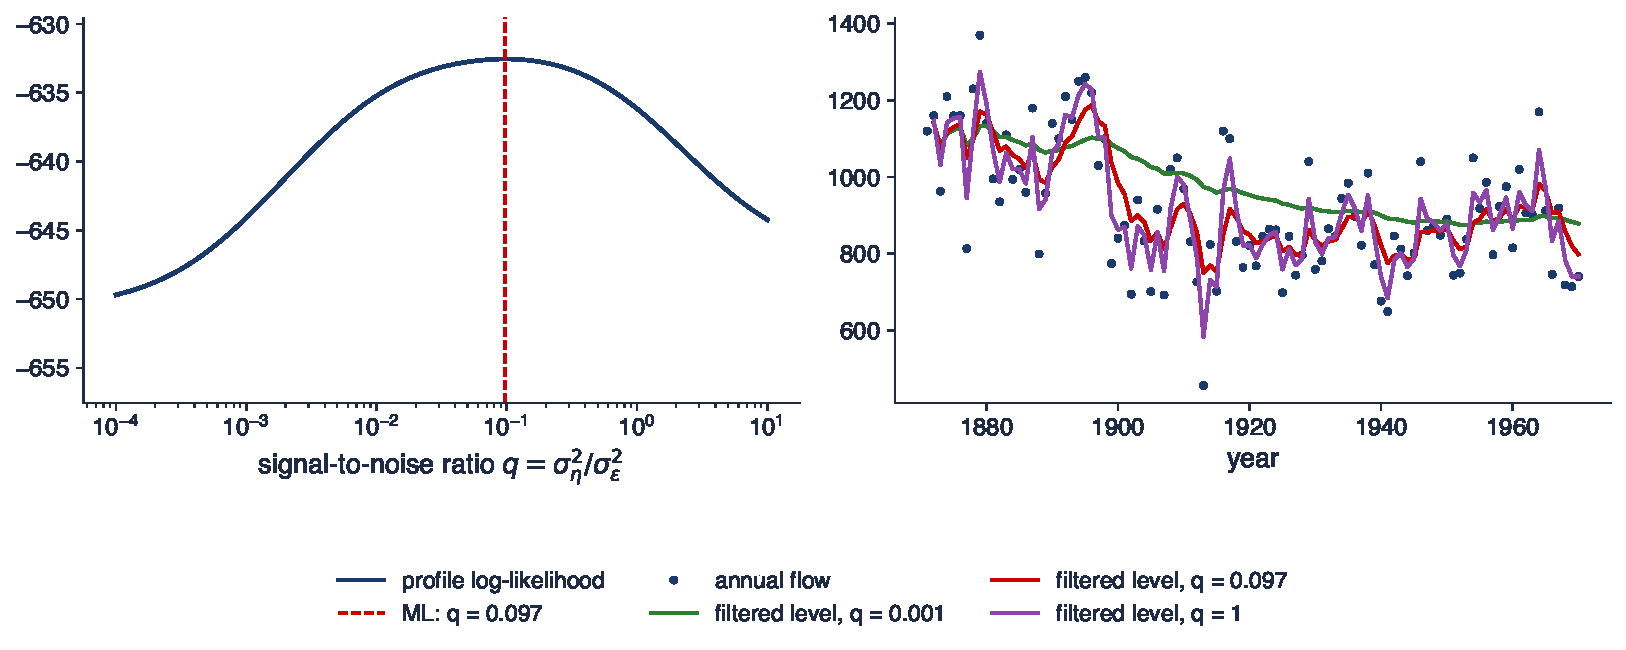
\includegraphics[width=0.97\textwidth,height=0.66\textheight,keepaspectratio]{tsa_ch10_likelihood.pdf}
\end{center}
\vspace{-0.25cm}
\begin{itemize}
    \item Stînga: log-verosimilitatea profil a modelului local level pentru Nil, în funcție de $q$ (scară logaritmică); dreapta: nivelurile filtrate pentru $q = 0{,}001$, valoarea ML și $q = 1$
\end{itemize}
\quantlet{TSA\_ch10\_smoothing\_likelihood}{\qlurl{TSA_ch10_smoothing_likelihood}}
\end{frame}

\begin{frame}{Interpretarea verosimilității profil}
\itemsize{\small}
\begin{itemize}
    \item Un maxim clar la $\hat q = 0{,}097$, cu $\hat\sigma^2_\varepsilon = 15100$ din forma închisă
    \begin{itemize}
        \item statistica raportului de verosimilitate față de $q = 0{,}001$ (un nivel aproape constant): 23{,}1; față de $q = 1$: 7{,}2
    \end{itemize}
    \item $q$ mic: nivelul este aproape plat și nu surprinde scăderea de după 1899; $q$ mare: nivelul urmărește fiecare viitură
    \begin{itemize}
        \item verosimilitatea alege compromisul care prezice cel mai bine la un pas
    \end{itemize}
    \item Alegerea lui $q$ este echivalentă cu alegerea ponderii SES $\alpha$ din \tsachlink{https://danpele.github.io/Time-Series-Analysis/RO/Cursuri/capitol0_introducere.pdf}{Capitolul 0}, acum cu un criteriu statistic
\end{itemize}
\end{frame}

\begin{frame}{Diagnosticare}
\itemsize{\small}
\begin{itemize}
    \item Dacă modelul este corect, erorile de predicție standardizate $e_t = v_t/\sqrt{F_t}$ sînt i.i.d. $N(0, 1)$
    \begin{itemize}
        \item verificările din \tsachlink{https://danpele.github.io/Time-Series-Analysis/RO/Cursuri/capitol1_procese_stochastice_stationaritate.pdf}{Capitolele 1}--\tsachlink{https://danpele.github.io/Time-Series-Analysis/RO/Cursuri/capitol2_modele_arma.pdf}{2}: ACF și testul Ljung--Box (independență), Jarque--Bera (normalitate), graficul în timp (valori extreme)
    \end{itemize}
    \item \textbf{Reziduurile auxiliare} \refDK: perturbațiile netezite $\hat\varepsilon_t$ și $\hat\eta_t$, standardizate
    \begin{itemize}
        \item un $\hat\varepsilon_t$ mare: o \textbf{valoare extremă} într-o singură observație
        \item un $\hat\eta_t$ mare: o \textbf{ruptură} în nivel, o deplasare permanentă
    \end{itemize}
    \item Se calculează printr-o recursie înapoi (netezitorul perturbațiilor) după filtru
\end{itemize}
\end{frame}

\begin{frame}{Diagnosticarea modelului pentru Nil}
\itemsize{\footnotesize}
\begin{center}
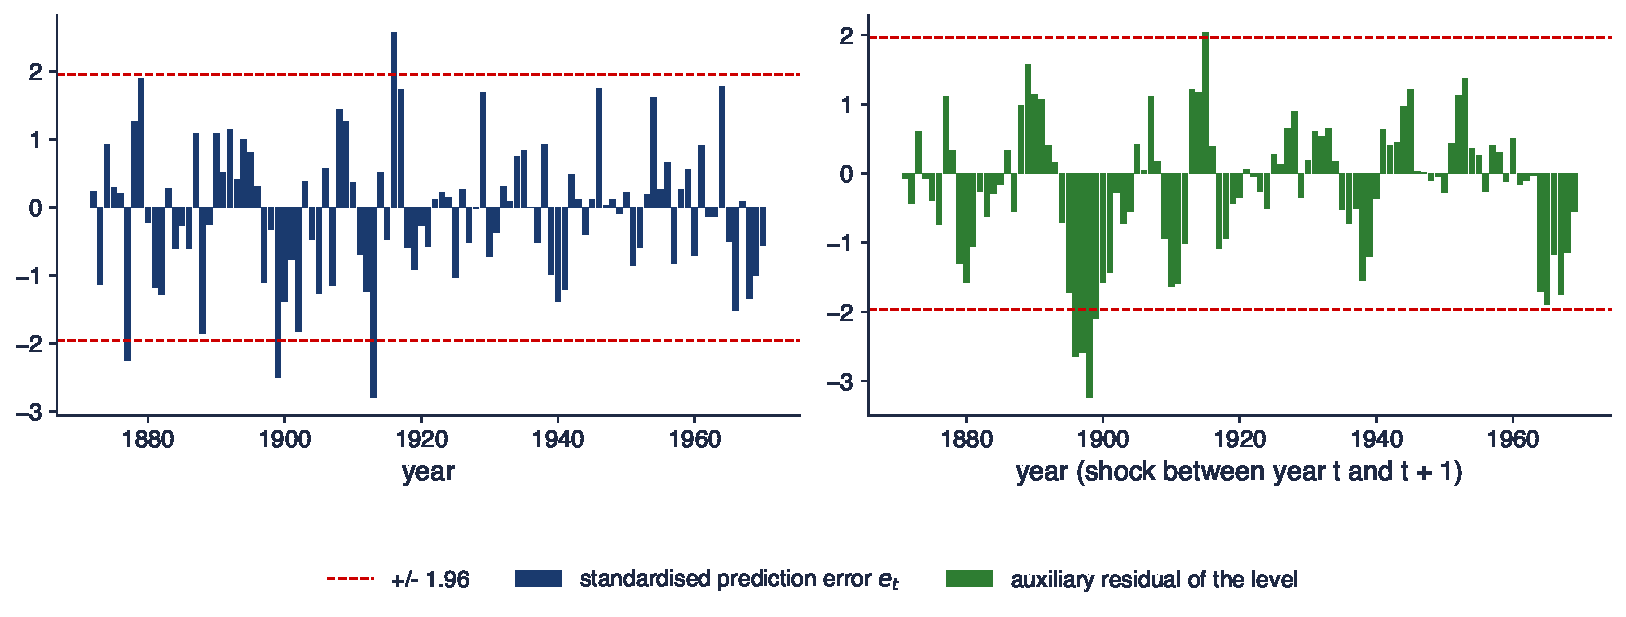
\includegraphics[width=0.97\textwidth,height=0.66\textheight,keepaspectratio]{tsa_ch10_diagnostics.pdf}
\end{center}
\vspace{-0.25cm}
\begin{itemize}
    \item Stînga: erorile de predicție la un pas standardizate $e_t$; dreapta: reziduul auxiliar standardizat al nivelului, $\hat\eta_t$ (un șoc între anul $t$ și $t+1$); linie punctată: $\pm 1{,}96$
\end{itemize}
\quantlet{TSA\_ch10\_smoothing\_likelihood}{\qlurl{TSA_ch10_smoothing_likelihood}}
\end{frame}

\begin{frame}{Interpretarea diagnosticării}
\itemsize{\small}
\begin{itemize}
    \item Erorile de predicție: Ljung--Box $Q(10) = 13{,}2$ (p = 0{,}21), Jarque--Bera 0{,}05 (p = 0{,}98); 4 din 99 în afara intervalului $\pm 1{,}96$
    \begin{itemize}
        \item nicio dovadă împotriva modelului în erorile la un pas
    \end{itemize}
    \item Reziduul nivelului are minimul în 1898 (\ensuremath{-}3{,}23): deplasarea nivelului între 1898 și 1899
    \begin{itemize}
        \item reziduul observației are minimul în 1913 (\ensuremath{-}3{,}04): un singur an foarte secetos, o valoare extremă
    \end{itemize}
    \item Aceeași ruptură ca în \tsachlink{https://danpele.github.io/Time-Series-Analysis/RO/Cursuri/capitol8_memorie_lunga_arfima.pdf}{Capitolul 8} (memoria lungă aparentă a Nilului), acum localizată de model însuși
\end{itemize}
\end{frame}

\begin{frame}{Valori lipsă și prognoză}
\itemsize{\small}
\begin{itemize}
    \item Un $y_t$ lipsă: fără actualizare; $a_{t+1} = Ta_t$, $P_{t+1} = TP_tT' + RQR'$
    \begin{itemize}
        \item verosimilitatea omite pur și simplu acel termen; nu interpolăm nimic de mînă
    \end{itemize}
    \item Prognoza la $h$ pași = tratarea lui $y_{n+1}, \dots, y_{n+h}$ ca valori lipsă
    \begin{itemize}
        \item local level: $\hat y_{n+h} = a_{n+1}$ pentru orice $h$, cu varianța $P_{n+1} + (h-1)\sigma^2_\eta + \sigma^2_\varepsilon$
    \end{itemize}
    \item Utilizări: date neregulate (sărbători), serii care încep la date diferite, frecvențe mixte, marginea neregulată a unui nowcast
    \begin{itemize}
        \item netezitorul umple golurile cu $\hat\alpha_t$ și cu eroarea standard corespunzătoare
    \end{itemize}
\end{itemize}
\end{frame}

\begin{frame}{Ani lipsă și prognoze pentru Nil}
\itemsize{\footnotesize}
\begin{center}
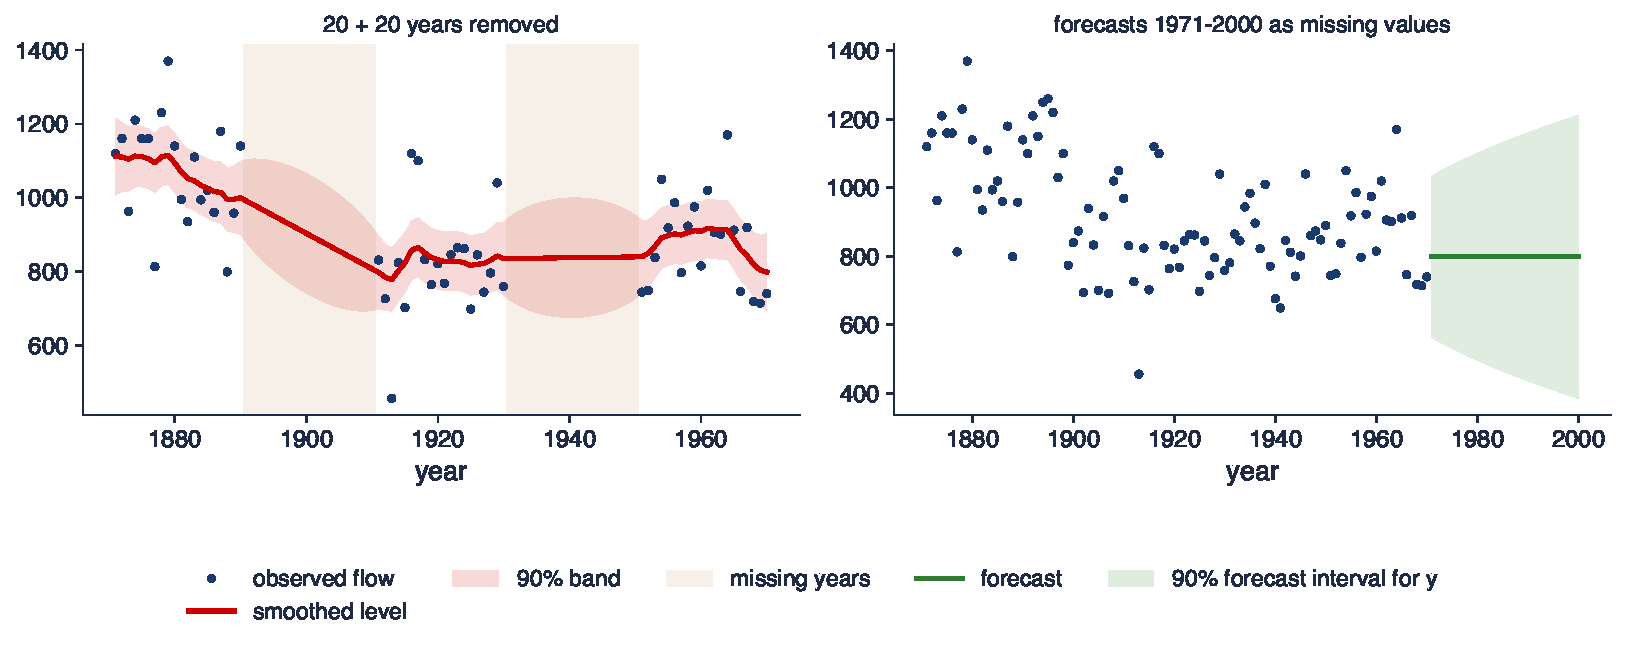
\includegraphics[width=0.97\textwidth,height=0.66\textheight,keepaspectratio]{tsa_ch10_missing.pdf}
\end{center}
\vspace{-0.25cm}
\begin{itemize}
    \item Stînga: anii 1891--1910 și 1931--1950 eliminați (experimentul din \refDK), nivelul netezit cu banda de 90\%; dreapta: prognozele pentru 1971--2000, cu intervale de 90\% pentru $y$
\end{itemize}
\quantlet{TSA\_ch10\_missing\_data}{\qlurl{TSA_ch10_missing_data}}
\end{frame}

\begin{frame}{Interpretarea valorilor lipsă}
\itemsize{\small}
\begin{itemize}
    \item În interiorul unui gol nivelul netezit este o dreaptă între cele două margini; eroarea standard crește la 99 în 1900, față de 48 cu toate datele
    \begin{itemize}
        \item banda se lărgește spre mijlocul golului și se îngustează lîngă anii observați
    \end{itemize}
    \item Prognozele sînt constante, la 798: un nivel de tip mers aleator nu are o direcție previzibilă
    \begin{itemize}
        \item eroarea standard a lui $y$: 144 la un an, 251 după 30 de ani
    \end{itemize}
    \item Același cod tratează valorile lipsă, prognozele și estimarea: unul dintre principalele avantaje practice ale modelelor în spațiul stărilor
\end{itemize}
\end{frame}

\begin{frame}{Recapitulare: netezire, verosimilitate și valori lipsă}
\itemsize{\small}
\begin{itemize}
    \item Filtrat: timp real; netezit (RTS): tot eșantionul, varianță mai mică
    \item $\log L = -\frac12\sum(\log 2\pi + \log F_t + v_t^2/F_t)$, maximizată numeric
    \item Diagnosticare pe $e_t$; reziduurile auxiliare găsesc valori extreme și rupturi (Nilul, 1898--1899)
    \item Valori lipsă și prognoze: sărim peste pasul de actualizare
\end{itemize}
\end{frame}


%=============================================================================
\section{Trend, ciclu și factori comuni}
%=============================================================================

\begin{frame}{Modele cu componente neobservate}
\itemsize{\small}
\begin{itemize}
    \item Modelul \textbf{structural de serii de timp} sau \textbf{cu componente neobservate} (UC) \refHarvey: $y_t = \mu_t + \psi_t + \gamma_t + \varepsilon_t$
    \begin{itemize}
        \item trend $\mu_t$ (local level sau local linear trend), ciclu $\psi_t$, sezonalitate $\gamma_t$, componenta neregulată $\varepsilon_t$
        \item descompunerea din \tsachlink{https://danpele.github.io/Time-Series-Analysis/RO/Cursuri/capitol0_introducere.pdf}{Capitolul 0}, dar fiecare componentă este un proces stochastic cu propria varianță
    \end{itemize}
    \item \textbf{Ciclul}: un AR(2) staționar $\psi_t = \phi_1\psi_{t-1} + \phi_2\psi_{t-2} + \kappa_t$ sau un ciclu stochastic amortizat cu perioada $2\pi/\lambda_c$
    \begin{itemize}
        \item $\phi_1$, $\phi_2$: coeficienții AR ai ciclului; $\kappa_t$: șocul ciclului; $\lambda_c$: frecvența ciclului, în radiani
        \item pentru logaritmul PIB, $\psi_t$ este \textbf{deviația PIB} (output gap): abaterea procentuală a producției de la trend (potențial)
    \end{itemize}
    \item În Python: \texttt{UnobservedComponents(y, level='smooth trend', autoregressive=2)}; toată starea se estimează cu filtrul și netezitorul Kalman
\end{itemize}
\end{frame}

\begin{frame}{Filtrul HP este un netezitor în spațiul stărilor}
\itemsize{\small}
\begin{itemize}
    \item \refHPf: trendul $\tau_t$ minimizează $\sum_t(y_t - \tau_t)^2 + \lambda\sum_t(\Delta^2\tau_t)^2$; $\lambda = 1600$ pentru date trimestriale
    \begin{itemize}
        \item $\Delta^2\tau_t = \tau_t - 2\tau_{t-1} + \tau_{t-2}$: variația pantei trendului; $\lambda \ge 0$: parametrul de netezire
        \item $\lambda$ mare: un trend liniar; $\lambda = 0$: trendul este chiar seria
    \end{itemize}
    \item Este exact trendul \textbf{netezit} al unui model UC: trend neted ($\Delta^2\mu_{t+1} = \zeta_t$) plus zgomot alb, cu $\lambda = \sigma^2_\varepsilon/\sigma^2_\zeta$ \refHJ
    \begin{itemize}
        \item filtrul HP impune raportul semnal--zgomot și o deviație de tip zgomot alb; modelul UC le estimează pe amîndouă
    \end{itemize}
    \item Fiind un netezitor, HP folosește date viitoare: ultimele lui valori se revizuiesc pe măsură ce sosesc trimestre noi
\end{itemize}
\end{frame}

\begin{frame}{Hamilton (2018): argumentele împotriva filtrului HP}
\itemsize{\small}
\begin{itemize}
    \item \refHamHP\ enumeră trei probleme
    \begin{itemize}
        \item deviația HP a unui mers aleator are cicluri care nu există în date: dinamică aparentă
        \item sfîrșitul eșantionului este tratat altfel decît mijlocul: revizuiri mari, deviații înșelătoare în timp real
        \item $\lambda = 1600$ este o convenție, departe de valoarea pe care ar alege-o o verosimilitate
    \end{itemize}
    \item Alternativa lui, \textbf{filtrul de regresie}: OLS a lui $y_{t+h}$ pe $1, y_t, y_{t-1}, y_{t-2}, y_{t-3}$, cu $h = 8$ trimestre
    \begin{itemize}
        \item ciclul este reziduul: ceea ce nu putea fi prezis cu doi ani înainte; unilateral prin construcție
    \end{itemize}
    \item Nicio metodă nu dă valoarea adevărată: comparăm modelul UC, HP și filtrul Hamilton pe PIB-ul României
\end{itemize}
\end{frame}

\begin{frame}{PIB-ul României: trendul}
\itemsize{\footnotesize}
\begin{center}
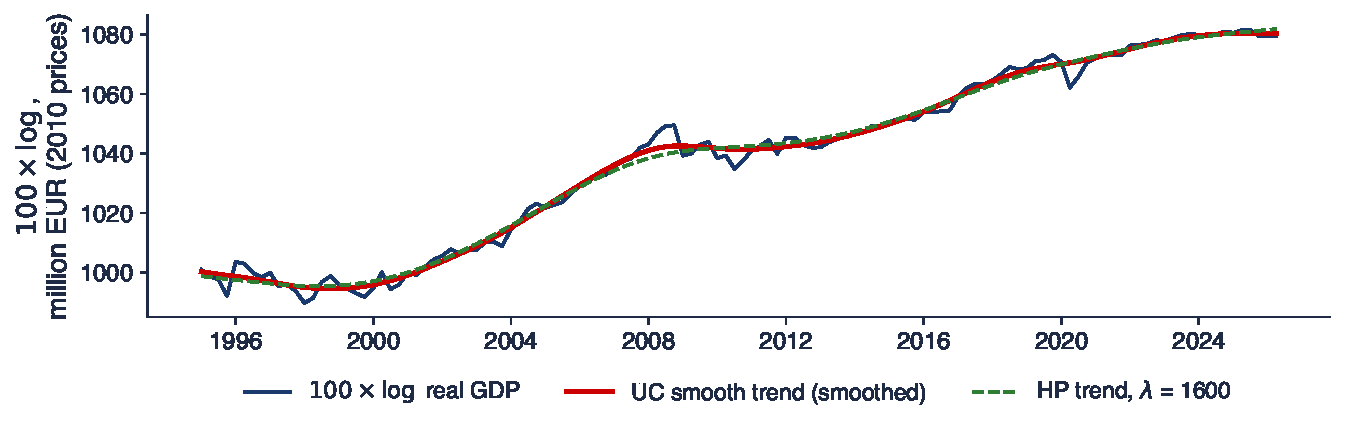
\includegraphics[width=0.97\textwidth,height=0.58\textheight,keepaspectratio]{tsa_ch10_ro_trend.pdf}
\end{center}
\vspace{-0.25cm}
\begin{itemize}
    \item $100 \times \log$ din PIB-ul real, trimestrial, ajustat sezonier și cu numărul de zile lucrătoare, volume înlănțuite (Eurostat namq\_10\_gdp), T1 1995--T2 2026 ($T = 126$); modelul UC: trend neted plus ciclu AR(2); HP cu $\lambda = 1600$
\end{itemize}
\quantlet{TSA\_ch10\_trend\_cycle}{\qlurl{TSA_ch10_trend_cycle}}
\end{frame}

\begin{frame}{Interpretarea trendului}
\itemsize{\small}
\begin{itemize}
    \item Creștere medie de 2{,}5\% pe an, cu un început lent (recesiunea din 1997--1999), un boom pînă în 2008, o stagnare și o revenire după 2013
    \begin{itemize}
        \item cele două trenduri sînt aproape identice: diferența dintre metode se află în deviație, nu în trend
    \end{itemize}
    \item Estimările UC: $\hat\sigma^2_\zeta = 0{,}078$ (panta trendului), ciclul AR(2) cu $\hat\phi_1 = 0{,}61$, $\hat\phi_2 = \ensuremath{-}0{,}13$, $\hat\sigma^2_\kappa = 5{,}27$; varianța componentei neregulate este estimată la zero
    \begin{itemize}
        \item raportul dintre varianța ciclului și varianța trendului este 68, mult sub valoarea 1600 impusă de HP: un trend mai flexibil
    \end{itemize}
    \item Un trend flexibil absoarbe o parte din boom: deviația UC va fi mai mică decît deviația HP
\end{itemize}
\end{frame}

\begin{frame}{Deviația PIB a României: trei metode}
\itemsize{\footnotesize}
\begin{center}
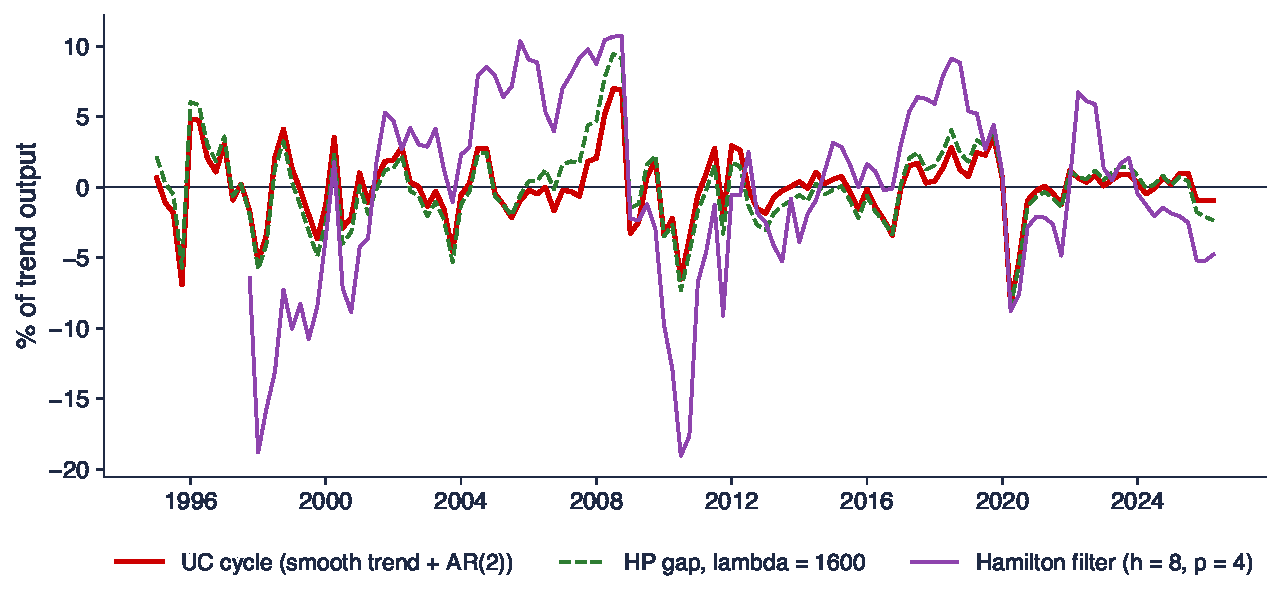
\includegraphics[width=0.97\textwidth,height=0.58\textheight,keepaspectratio]{tsa_ch10_output_gap.pdf}
\end{center}
\vspace{-0.25cm}
\begin{itemize}
    \item Deviația în \% din trend: ciclul UC (netezit), deviația HP ($\lambda = 1600$) și filtrul Hamilton ($h = 8$, patru laguri), primele 11 trimestre se pierd
\end{itemize}
\quantlet{TSA\_ch10\_trend\_cycle}{\qlurl{TSA_ch10_trend_cycle}}
\end{frame}

\begin{frame}{Interpretarea deviațiilor PIB}
\itemsize{\small}
\begin{itemize}
    \item Toate cele trei metode surprind supraîncălzirea dinainte de 2008 (maxime: UC 7{,}0\% în T3 2008, HP 9{,}5\%, Hamilton 10{,}7\%) și pandemia din 2020 (UC \ensuremath{-}8{,}3\%, HP \ensuremath{-}8{,}5\%)
    \begin{itemize}
        \item corelații: UC--HP 0{,}94, UC--Hamilton 0{,}57, HP--Hamilton 0{,}69
    \end{itemize}
    \item Abaterile standard: UC 2{,}4, HP 2{,}9, Hamilton 6{,}5: deviația Hamilton conține și toate surprizele din doi ani
    \begin{itemize}
        \item cei patru coeficienți ai regresiei au suma 0{,}97: PIB-ul este aproape de un mers aleator cu derivă
    \end{itemize}
    \item Ultima deviație (T2 2026): UC \ensuremath{-}0{,}9\%, HP \ensuremath{-}2{,}4\%, Hamilton \ensuremath{-}4{,}8\%: semnul coincide, mărimea nu
\end{itemize}
\end{frame}

\begin{frame}{Timp real și retrospectivă}
\itemsize{\footnotesize}
\begin{center}
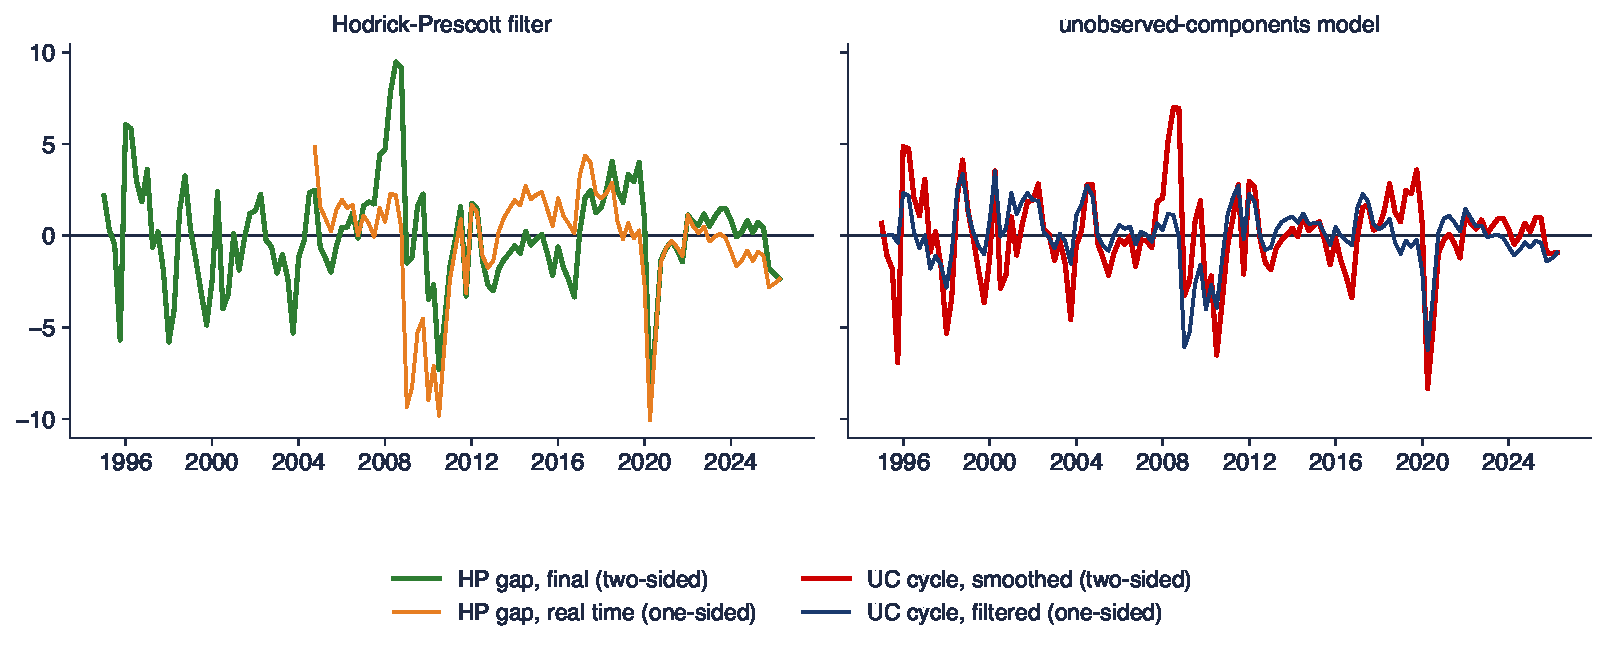
\includegraphics[width=0.97\textwidth,height=0.66\textheight,keepaspectratio]{tsa_ch10_realtime.pdf}
\end{center}
\vspace{-0.25cm}
\begin{itemize}
    \item Stînga: deviația HP calculată cu toate datele (bilaterală) și ultima valoare a deviației HP calculate cu datele disponibile la fiecare dată (unilaterală, din 2004); dreapta: ciclul UC, filtrat și netezit
\end{itemize}
\quantlet{TSA\_ch10\_trend\_cycle}{\qlurl{TSA_ch10_trend_cycle}}
\end{frame}

\begin{frame}{Interpretarea revizuirilor}
\itemsize{\small}
\begin{itemize}
    \item În T3 2008 deviația HP în timp real era 2{,}2\%; retrospectiv este 9{,}5\%: supraîncălzirea era invizibilă în timp real
    \begin{itemize}
        \item modelul UC arată aceeași problemă: filtrat 1{,}1\%, netezit 7{,}0\%
    \end{itemize}
    \item Revizuirea medie pătratică din 2004: HP 2{,}8 puncte, UC 1{,}8 puncte; corelația timp real--final: HP 0{,}57, UC 0{,}65
    \begin{itemize}
        \item problema capătului de eșantion din \refHamHP; modelul UC își raportează cel puțin propria incertitudine
    \end{itemize}
    \item Pentru politica economică în timp real folosiți estimarea filtrată (unilaterală) și eroarea ei standard, niciodată ultimul punct al unui filtru bilateral
\end{itemize}
\end{frame}

\begin{frame}{Un beta variabil în timp: BET și zona euro}
\itemsize{\footnotesize}
\begin{center}
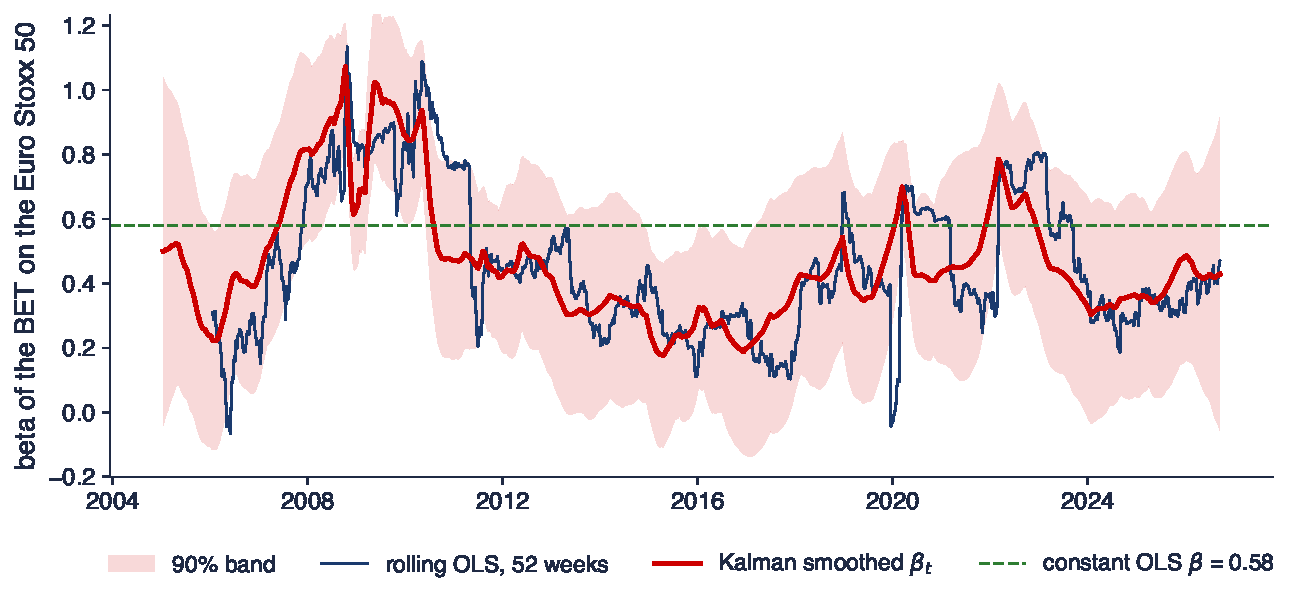
\includegraphics[width=0.97\textwidth,height=0.55\textheight,keepaspectratio]{tsa_ch10_tvp_beta.pdf}
\end{center}
\vspace{-0.25cm}
\begin{itemize}
    \item Randamentele logaritmice săptămînale ale BET pe Euro Stoxx 50 (EODHD), 2005--2026 ($T = 1\,126$ de săptămîni)
    \item Beta de tip mers aleator prin verosimilitate maximă, netezit Kalman, cu bandă de 90\%; OLS pe ferestre mobile de 52 de săptămîni; OLS constant
\end{itemize}
\quantlet{TSA\_ch10\_tvp\_regression}{\qlurl{TSA_ch10_tvp_regression}}
\end{frame}

\begin{frame}{Interpretarea coeficientului beta variabil}
\itemsize{\small}
\begin{itemize}
    \item Beta OLS constant este 0{,}58; beta netezit atinge 1{,}07 (octombrie 2008) și coboară la 0{,}17 (aprilie 2015)
    \begin{itemize}
        \item în criza din 2008 piața românească s-a mișcat aproape unu la unu cu zona euro; ulterior s-a decuplat
    \end{itemize}
    \item Raportul de verosimilitate față de un beta constant: 46{,}1 (o restricție, o varianță la limită): dovezi puternice de variație
    \begin{itemize}
        \item abaterea standard săptămînală a șocurilor lui beta 0{,}059; ultimul beta 0{,}43, cu eroarea standard 0{,}29
    \end{itemize}
    \item Estimarea pe fereastră mobilă se modifică brusc cînd o singură săptămînă extremă intră sau iese din fereastră; beta Kalman se mișcă doar atît cît permite verosimilitatea
\end{itemize}
\end{frame}

\begin{frame}{Modele cu factori dinamici și nowcasting}
\itemsize{\small}
\begin{itemize}
    \item \textbf{Model cu factori dinamici}: $y_{it} = \lambda_if_t + u_{it}$, \quad $f_t = \phi_1f_{t-1} + \phi_2f_{t-2} + \eta_t$
    \begin{itemize}
        \item multe serii $y_{1t}, \dots, y_{Nt}$ conduse de un factor comun neobservat $f_t$ (starea), cu încărcările $\lambda_i$
        \item $u_{it}$: partea seriei $i$ neexplicată de factor; $\phi_1$, $\phi_2$: coeficienții AR ai factorului
        \item \refSW: un indice coincident al activității din SUA, din patru indicatori lunari
    \end{itemize}
    \item \textbf{Nowcasting} \refGRS: estimăm trimestrul curent înainte ca PIB-ul să fie publicat
    \begin{itemize}
        \item datele lunare sosesc la date diferite: ultimele luni ale unor serii lipsesc (\textbf{marginea neregulată})
        \item filtrul Kalman le tratează ca valori lipsă și actualizează factorul cu ce a sosit deja
    \end{itemize}
    \item Băncile centrale folosesc astfel de modele pentru nowcasting-ul PIB; \texttt{statsmodels} are \texttt{DynamicFactor} și \texttt{DynamicFactorMQ}
\end{itemize}
\end{frame}

\begin{frame}{Un factor comun al activității din SUA}
\itemsize{\footnotesize}
\begin{center}
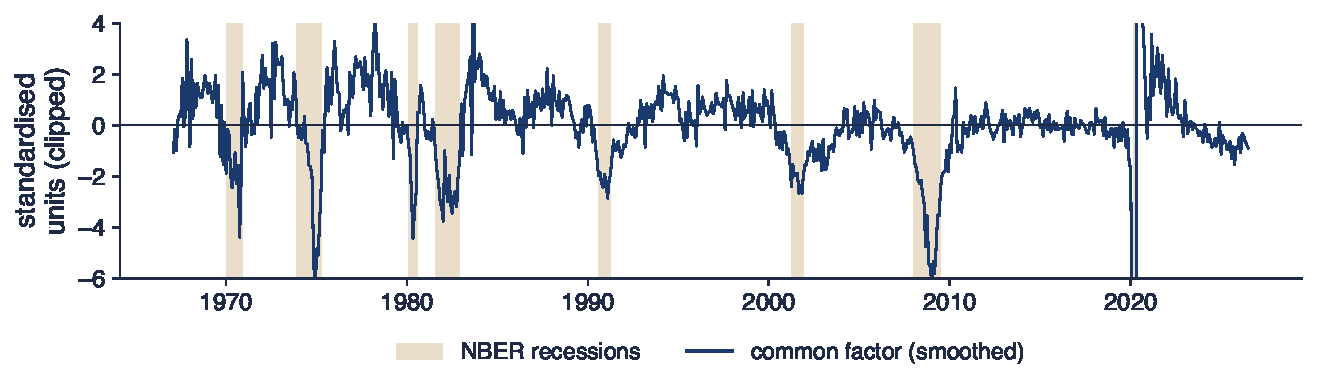
\includegraphics[width=0.97\textwidth,height=0.52\textheight,keepaspectratio]{tsa_ch10_dfm.pdf}
\end{center}
\vspace{-0.25cm}
\begin{itemize}
    \item Creșterea lunară a producției industriale, a numărului de salariați, a venitului real fără transferuri și a vînzărilor reale din industrie și comerț (FRED), standardizate
    \item Un factor AR(2) estimat pe 1967--2019 și rulat pînă în iulie 2026; ultimele două luni ale venitului și vînzărilor sînt tratate ca lipsă
\end{itemize}
\quantlet{TSA\_ch10\_dynamic\_factor}{\qlurl{TSA_ch10_dynamic_factor}}
\end{frame}

\begin{frame}{Interpretarea factorului comun}
\itemsize{\small}
\begin{itemize}
    \item Încărcări: salariați 0{,}59, producția industrială 0{,}42, vînzări 0{,}29, venit 0{,}23; factorul AR(2) cu $\hat\phi_1 = 0{,}42$, $\hat\phi_2 = 0{,}41$
    \begin{itemize}
        \item corelația cu media simplă a celor patru serii: 0{,}86
    \end{itemize}
    \item Media factorului: \ensuremath{-}3{,}5 în lunile de recesiune NBER, 0{,}4 în expansiuni; negativ în 99\% din lunile de recesiune
    \begin{itemize}
        \item aprilie 2020: \ensuremath{-}74 unități standard, în afara scalei graficului
    \end{itemize}
    \item Ultima valoare (iulie 2026): \ensuremath{-}0{,}9, calculată deși două dintre cele patru serii nu sînt încă disponibile
\end{itemize}
\end{frame}

\begin{frame}{Recapitulare: trend, ciclu și factori comuni}
\itemsize{\small}
\begin{itemize}
    \item Modelele UC: trend + ciclu + sezonalitate + componentă neregulată, fiecare cu varianța ei
    \item HP = netezitorul unui model UC cu $\lambda$ impus; Hamilton (2018): cicluri aparente și revizuiri la capătul eșantionului
    \item Deviația PIB a României: metodele coincid ca semn, nu ca mărime; deviațiile în timp real se revizuiesc puternic
    \item Regresia TVP și factorii dinamici sînt și ei modele în spațiul stărilor
\end{itemize}
\end{frame}


%=============================================================================
\section{Modele Markov switching}
%=============================================================================

\begin{frame}{Hamilton (1989) și datarea recesiunilor}
\itemsize{\footnotesize}
\begin{columns}[T]
\begin{column}{0.4\textwidth}
\centering
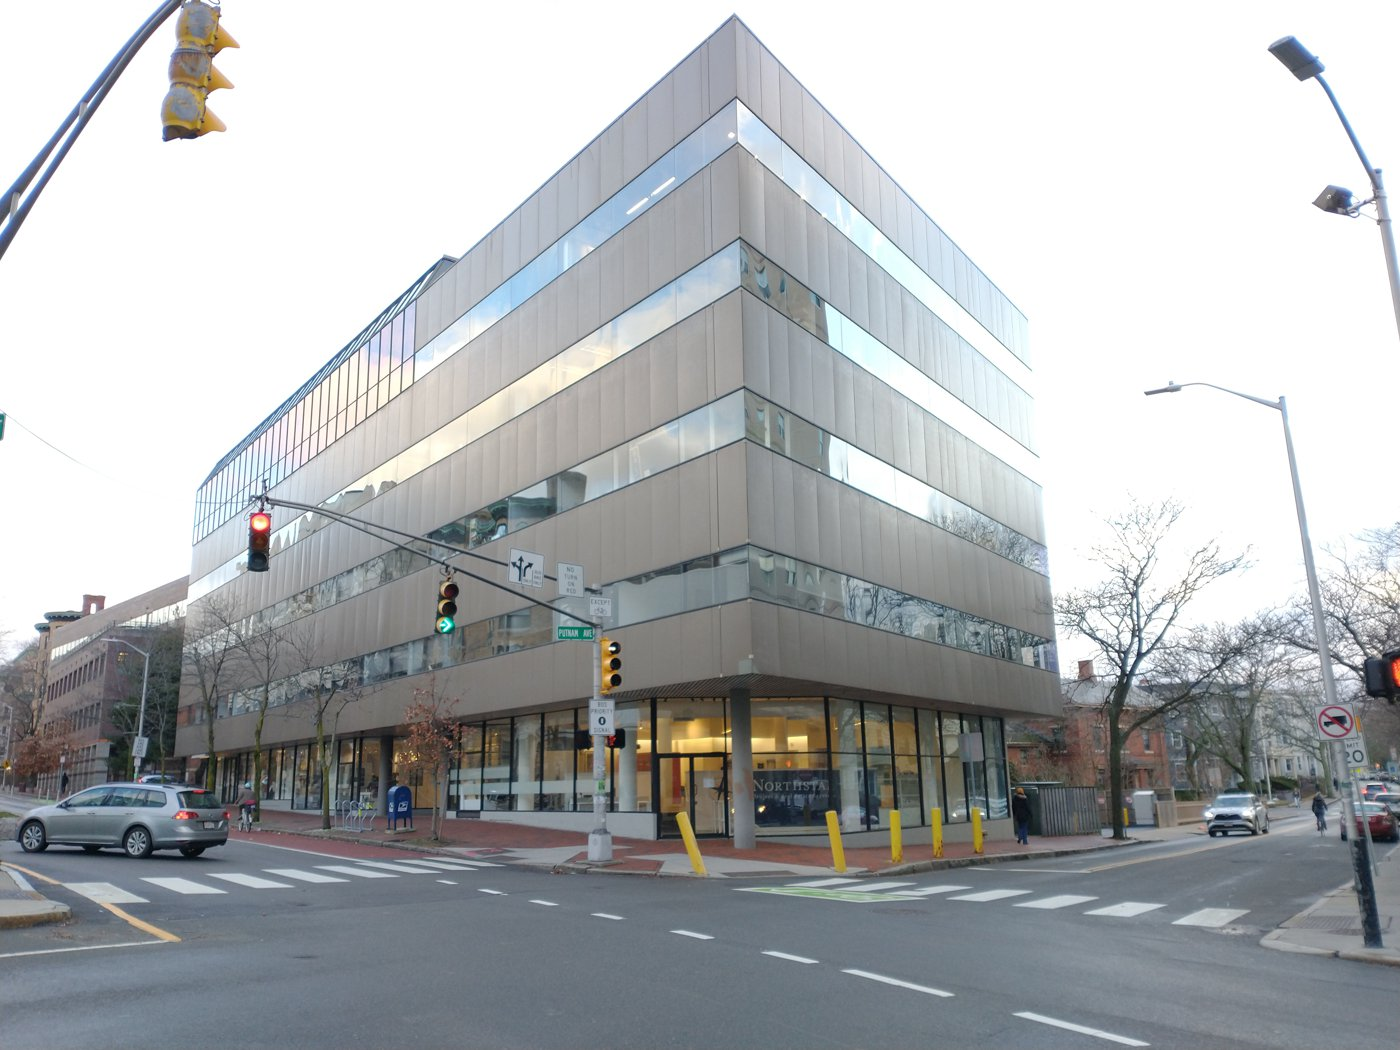
\includegraphics[height=0.36\textheight]{ch10_nber_offices_2022.jpg}\\[1mm]
\imgcap{NBER, Cambridge (Massachusetts), al cărui comitet datează recesiunile din SUA}
\imgcredit{https://commons.wikimedia.org/wiki/File:National_Bureau_of_Economic_Research_offices.jpg}{Foto: Astrophobe (2022); CC BY-SA 4.0; Wikimedia Commons}
\end{column}
\begin{column}{0.58\textwidth}
\begin{itemize}
    \item National Bureau of Economic Research (NBER) datează recesiunile din SUA printr-un comitet, la cîteva luni după eveniment
    \begin{itemize}
        \item o recesiune este un regim: PIB-ul se comportă altfel cît timp durează
    \end{itemize}
    \item \refHamMS: media creșterii PIB depinde de un regim neobservat $S_t \in \{1, 2\}$, care urmează un lanț Markov
    \begin{itemize}
        \item datele ne spun apoi probabilitatea unei recesiuni în fiecare trimestru, fără comitet
    \end{itemize}
    \item Starea este acum \textbf{discretă}; filtrul Kalman este înlocuit de filtrul Hamilton
\end{itemize}
\end{column}
\end{columns}
\end{frame}

\begin{frame}{Modelul Markov switching}
\itemsize{\small}
\begin{itemize}
    \item \textbf{Medie cu schimbare de regim}: $y_t = \mu_{S_t} + \varepsilon_t$, \quad $\varepsilon_t \sim N(0, \sigma^2_{S_t})$, \quad $S_t \in \{1, \dots, k\}$
    \begin{itemize}
        \item \textbf{Lanțul Markov}: $p_{ij} = \Pr(S_t = j \mid S_{t-1} = i)$, constante în timp; rîndurile matricei de tranziție însumează 1
    \end{itemize}
    \item MS-AR(4) al lui Hamilton: $y_t - \mu_{S_t} = \sum_{j=1}^{4}\phi_j(y_{t-j} - \mu_{S_{t-j}}) + \varepsilon_t$
    \begin{itemize}
        \item dinamica AR rămîne aceeași; doar media se schimbă
    \end{itemize}
    \item Variante: varianță cu schimbare de regim (piețe calme și agitate), coeficienți AR cu schimbare de regim, $k = 3$ regimuri
    \begin{itemize}
        \item în Python: \texttt{MarkovRegression}, \texttt{MarkovAutoregression} (\texttt{statsmodels})
    \end{itemize}
    \item Un model neliniar: prognoza depinde de probabilitatea fiecărui regim
\end{itemize}
\end{frame}

\begin{frame}{Matricea de tranziție, durate și probabilități ergodice}
\itemsize{\small}
\begin{itemize}
    \item Două regimuri: $\mathbf{P} = \begin{pmatrix}p_{11} & 1 - p_{11}\\ 1 - p_{22} & p_{22}\end{pmatrix}$
    \begin{itemize}
        \item tranzițiile în $h$ pași: $\mathbf{P}^h$
    \end{itemize}
    \item \textbf{Durata așteptată} a regimului $i$: timpul petrecut acolo este geometric, $\Pr(D = d) = p_{ii}^{d-1}(1 - p_{ii})$, deci $E(D) = 1/(1 - p_{ii})$
    \begin{itemize}
        \item $p_{11} = 0{,}75$: recesiunile durează în medie $1/0{,}25 = 4$ trimestre; $p_{22} = 0{,}95$: expansiunile durează 20 de trimestre
    \end{itemize}
    \item Probabilitățile \textbf{ergodice} (pe termen lung): $\pi_1 = \dfrac{1 - p_{22}}{2 - p_{11} - p_{22}}$, fracțiunea de timp petrecută în regimul 1
    \begin{itemize}
        \item exemplu: $\pi_1 = 0{,}05/0{,}30 = 1/6$: un trimestru din șase este trimestru de recesiune
    \end{itemize}
\end{itemize}
\end{frame}

\begin{frame}{Filtrul Hamilton}
\itemsize{\small}
\begin{itemize}
    \item Urmărim $\xi_{t|t} = \Pr(S_t = j \mid Y_t)$, \textbf{probabilitățile filtrate}, pentru fiecare regim $j$
    \begin{itemize}
        \item \textbf{predicția}: $\Pr(S_t = j \mid Y_{t-1}) = \sum_i p_{ij}\Pr(S_{t-1} = i \mid Y_{t-1})$
        \item \textbf{densitățile}: $f_j(y_t) = \varphi\bigl((y_t - \mu_j)/\sigma_j\bigr)/\sigma_j$, verosimilitatea lui $y_t$ în fiecare regim
        \item $\varphi$: densitatea distribuției Normale standard; $\mu_j$, $\sigma_j$: media și abaterea standard a regimului $j$
        \item \textbf{actualizarea} (Bayes): $\Pr(S_t = j \mid Y_t) = \dfrac{\Pr(S_t = j \mid Y_{t-1})\,f_j(y_t)}{\sum_i\Pr(S_t = i \mid Y_{t-1})\,f_i(y_t)}$
    \end{itemize}
    \item Numitorul este $p(y_t \mid Y_{t-1})$: log-verosimilitatea este $\sum_t\log p(y_t \mid Y_{t-1})$, ca la filtrul Kalman
    \begin{itemize}
        \item același ciclu predicție--actualizare, cu probabilități în locul mediilor și varianțelor
    \end{itemize}
    \item Pornirea: probabilitățile ergodice $\pi_j$
\end{itemize}
\end{frame}

\begin{frame}{Probabilități netezite și estimare}
\itemsize{\small}
\begin{itemize}
    \item \textbf{Probabilitățile netezite} $\Pr(S_t = j \mid Y_n)$: o trecere înapoi \refKim, analogul netezitorului RTS
    \begin{itemize}
        \item folosite pentru datarea istorică a regimurilor; probabilitățile filtrate sînt ceea ce știa un prognozator la momentul $t$
    \end{itemize}
    \item Estimarea: verosimilitate maximă prin optimizare numerică sau algoritmul EM \refHamEM
    \begin{itemize}
        \item EM: așteptarea (probabilitățile netezite pentru $\theta$ dat) și maximizarea (medii, varianțe și numărători de tranziții ponderate), repetate
    \end{itemize}
    \item Verosimilitatea are \textbf{mai multe maxime locale}: folosiți multe valori de pornire aleatoare și comparați soluțiile
    \begin{itemize}
        \item schimbarea etichetelor: regimurile 1 și 2 își pot schimba locul; denumiți-le după medii sau varianțe
    \end{itemize}
\end{itemize}
\end{frame}

\begin{frame}{Specificația lui Hamilton pe datele de azi}
\itemsize{\small}
\begin{center}
\footnotesize
\begin{tabular}{>{\raggedright\arraybackslash}p{5.6cm}cc}
\toprule
\textbf{MS-AR(4), creșterea PIB real al SUA, T2 1951--T4 1984} & \textbf{Maximul A} & \textbf{Maximul B} \\
\midrule
media, regimul 1 / regimul 2 (\% pe trimestru) & \ensuremath{-}0{,}14 / 1{,}32 & \ensuremath{-}1{,}14 / 0{,}96 \\
$p_{11}$, $p_{22}$ & 0{,}762; 0{,}892 & 0{,}128; 0{,}952 \\
durata așteptată, regimul 1 / 2 (trimestre) & 4{,}2 / 9{,}3 & 1{,}1 / 20{,}8 \\
log-verosimilitatea & \ensuremath{-}189{,}47 & \ensuremath{-}189{,}16 \\
trimestre de recesiune NBER găsite (prob. netezită $> 0{,}5$) & 94\% & 10\% \\
\bottomrule
\end{tabular}
\end{center}
\begin{itemize}
    \item Maximul A este răspunsul lui Hamilton: un regim de recesiune de aproximativ patru trimestre, care se potrivește cu datările NBER
    \item Maximul B are o verosimilitate puțin mai mare, dar alt înțeles: trimestre izolate cu scăderi bruște
    \item O diferență de verosimilitate de \ensuremath{-}189{,}16 față de \ensuremath{-}189{,}47 nu poate decide; decid înțelesul economic și verificările de robustețe
\end{itemize}
\end{frame}

\begin{frame}{Recesiunile din SUA din creșterea PIB}
\itemsize{\footnotesize}
\begin{center}
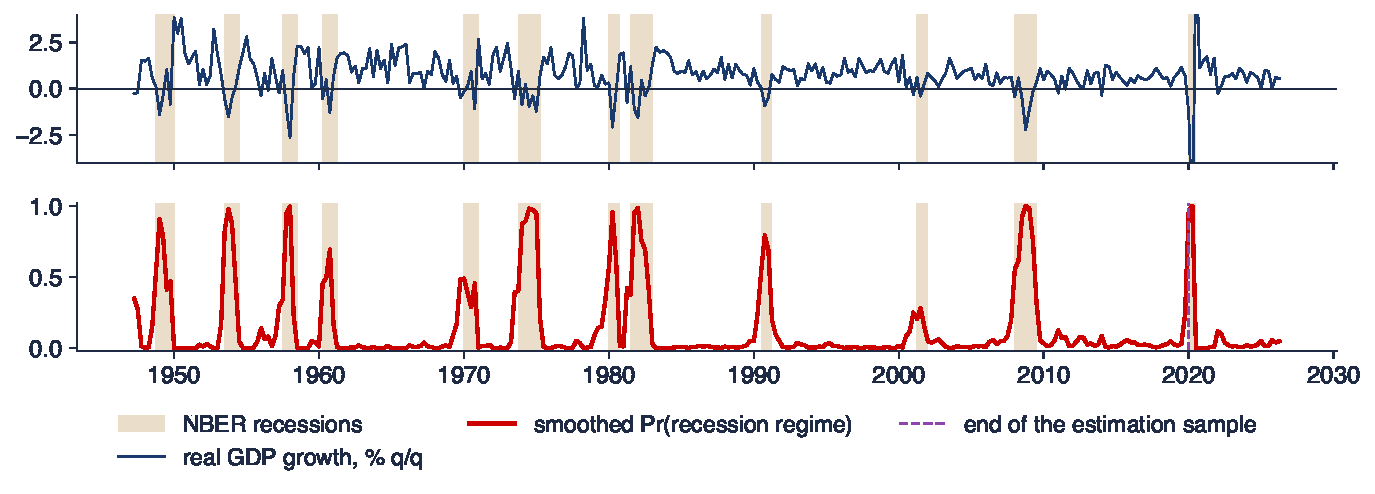
\includegraphics[width=0.97\textwidth,height=0.66\textheight,keepaspectratio]{tsa_ch10_ms_us.pdf}
\end{center}
\vspace{-0.25cm}
\begin{itemize}
    \item Două regimuri cu medie variabilă și varianță constantă, estimate pe T2 1947--T4 2019, eșantion cu 48 de trimestre de recesiune NBER (FRED GDPC1, USREC); probabilitățile de după 2019 sînt calculate cu aceiași parametri
\end{itemize}
\quantlet{TSA\_ch10\_markov\_gdp}{\qlurl{TSA_ch10_markov_gdp}}
\end{frame}

\begin{frame}{Interpretarea probabilităților de recesiune}
\itemsize{\small}
\begin{itemize}
    \item Mediile regimurilor: \ensuremath{-}0{,}42\% (recesiune) și 0{,}97\% (expansiune) pe trimestru, $\hat\sigma = 0{,}79$; $\hat p_{11} = 0{,}685$, $\hat p_{22} = 0{,}949$
    \begin{itemize}
        \item durate așteptate: 3{,}2 trimestre de recesiune, 19{,}7 trimestre de expansiune; ponderea ergodică a recesiunii 14\%
    \end{itemize}
    \item Concordanța cu NBER: 94\% din trimestre; 62\% din trimestrele de recesiune NBER detectate, 0\% alarme false
    \begin{itemize}
        \item modelul nu detectează recesiunile ușoare (2001), dar le detectează pe cele profunde
    \end{itemize}
    \item T2 2020 ($\ensuremath{-}8{,}2\%$): probabilitatea 1{,}00, apoi revenire la expansiune; după 2021 probabilitatea nu depășește 0{,}12
\end{itemize}
\end{frame}

\begin{frame}{Probabilități filtrate și netezite: 2008}
\itemsize{\footnotesize}
\begin{center}
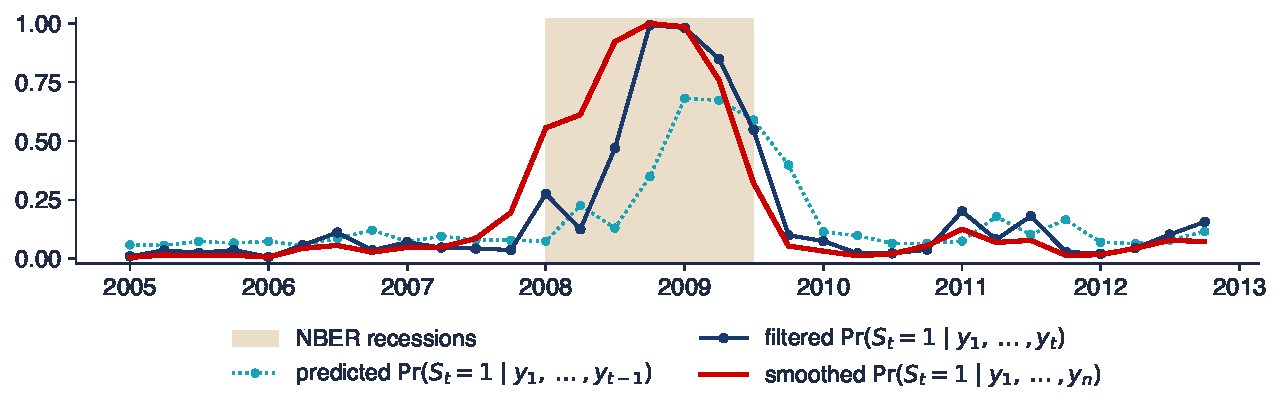
\includegraphics[width=0.97\textwidth,height=0.56\textheight,keepaspectratio]{tsa_ch10_ms_filtered.pdf}
\end{center}
\vspace{-0.25cm}
\begin{itemize}
    \item Probabilitatea prezisă, filtrată și netezită a regimului de recesiune, 2005--2012, același model ca în graficul anterior
\end{itemize}
\quantlet{TSA\_ch10\_markov\_gdp}{\qlurl{TSA_ch10_markov_gdp}}
\end{frame}

\begin{frame}{Interpretarea probabilităților în timp real}
\itemsize{\small}
\begin{itemize}
    \item Recesiunea NBER a început în T1 2008; probabilitatea netezită trece de 0,5 în T1 2008, cea filtrată abia în T4 2008
    \begin{itemize}
        \item T1 2008: filtrată 0{,}28, netezită 0{,}56; T3 2008 (creștere \ensuremath{-}0{,}53\%): filtrată 0{,}47, netezită 0{,}92
    \end{itemize}
    \item Concordanța cu NBER folosind doar probabilitățile filtrate: 92\% din trimestre, 54\% din trimestrele de recesiune
    \begin{itemize}
        \item datarea în timp real este mai grea: \refCP\ compară metodele pe date în timp real
    \end{itemize}
    \item Nu judecați niciodată capacitatea unui model în timp real după probabilitățile netezite: ele folosesc viitorul
\end{itemize}
\end{frame}

\begin{frame}{Verificări: regimurile găsite de model}
\itemsize{\small}
\begin{itemize}
    \item \textbf{Varianță cu schimbare de regim} pe 1947--2019: regimurile devin volatilitate mare și volatilitate mică, nu recesiune și expansiune
    \begin{itemize}
        \item abateri standard 1{,}20 și 0{,}44; durate de 45 și 39 de trimestre; trecerea la regimul calm în T3 1984
        \item aceasta este „Marea Moderație” de la mijlocul anilor 1980; concordanța cu NBER scade la 60\% (47\% alarme false)
    \end{itemize}
    \item \textbf{Includerea anului 2020} în estimare: un regim este doar trimestrul T2 2020 (media \ensuremath{-}8{,}2\%), celălalt durează 315 de trimestre
    \begin{itemize}
        \item o singură observație extremă poate forma singură un regim
    \end{itemize}
    \item Lista de verificări: reprezentați probabilitățile alături de evenimente cunoscute; comparați mai multe valori de pornire și eșantioane; preferați specificația cu un înțeles economic clar
\end{itemize}
\end{frame}

\begin{frame}{Regimuri ale creșterii PIB în România}
\itemsize{\footnotesize}
\begin{center}
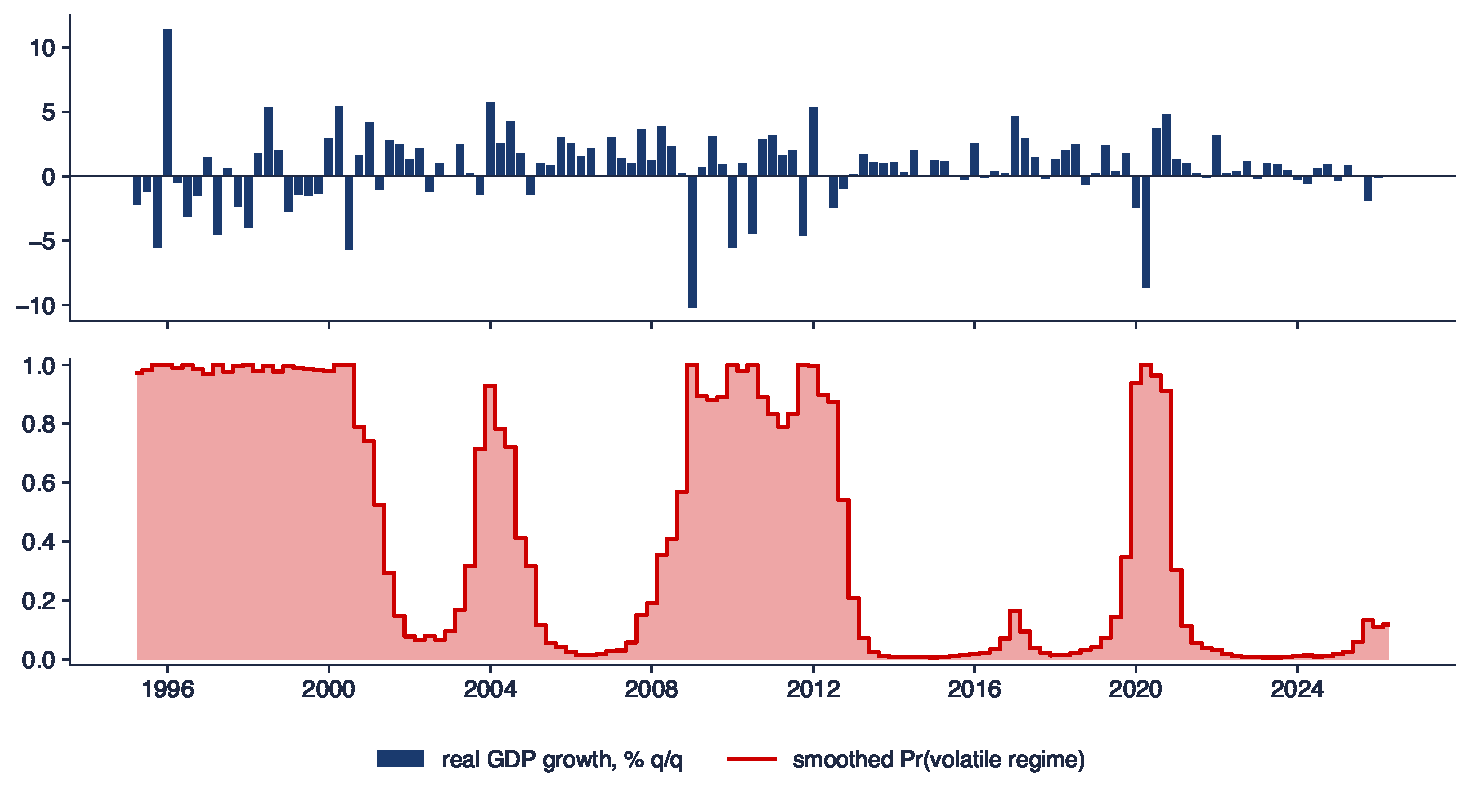
\includegraphics[width=0.97\textwidth,height=0.66\textheight,keepaspectratio]{tsa_ch10_ms_ro.pdf}
\end{center}
\vspace{-0.25cm}
\begin{itemize}
    \item Creșterea trimestrială a PIB-ului real al României (Eurostat), două regimuri cu medie și varianță variabile; probabilitatea netezită a regimului volatil
\end{itemize}
\quantlet{TSA\_ch10\_markov\_gdp}{\qlurl{TSA_ch10_markov_gdp}}
\end{frame}

\begin{frame}{Interpretarea regimurilor din România}
\itemsize{\small}
\begin{itemize}
    \item Regimul stabil: media 1{,}03\% pe trimestru, abaterea standard 1{,}3; regimul volatil: media 0{,}07\%, abaterea standard 3{,}9
    \begin{itemize}
        \item durate așteptate: 15{,}2 trimestre în regimul stabil, 11{,}2 trimestre în cel volatil; 40\% din trimestre sînt volatile
    \end{itemize}
    \item Episoade volatile: T2 1995--T2 2001 (tranziția și recesiunea din 1997--1999), T4 2003--T3 2004, T4 2008--T4 2012 (criza și austeritatea din 2010), T1 2020--T4 2020 (pandemia)
    \begin{itemize}
        \item ultima probabilitate a regimului volatil: 0{,}12
    \end{itemize}
    \item Cu 125 de trimestre un model doar cu medie variabilă este instabil; într-o economie emergentă regimurile de volatilitate și de creștere vin împreună
\end{itemize}
\end{frame}

\begin{frame}{Piețe bursiere calme și agitate}
\itemsize{\footnotesize}
\begin{center}
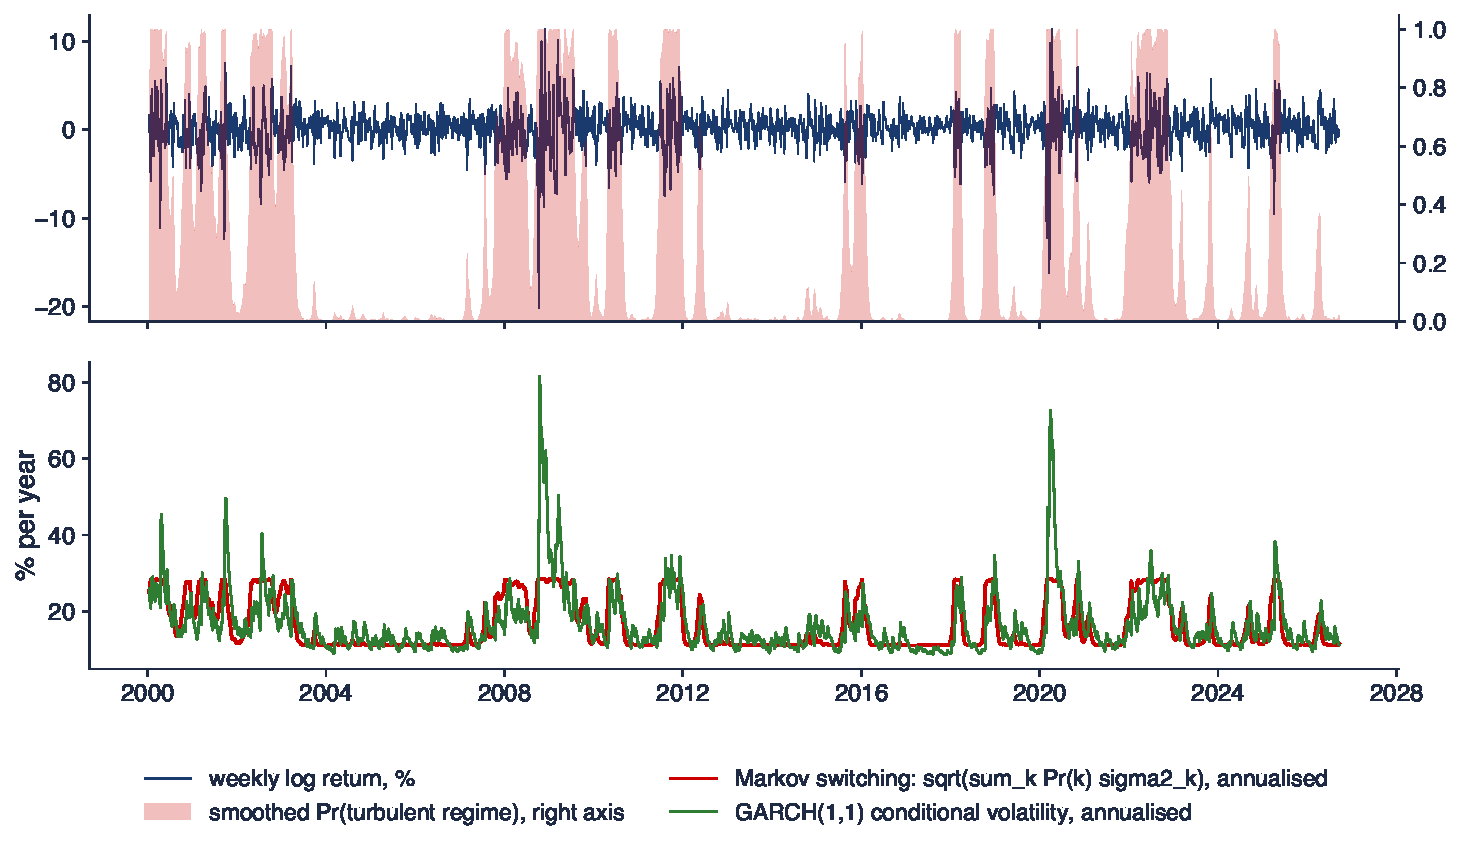
\includegraphics[width=0.97\textwidth,height=0.66\textheight,keepaspectratio]{tsa_ch10_vol_regimes.pdf}
\end{center}
\vspace{-0.25cm}
\begin{itemize}
    \item Randamentele logaritmice săptămînale ale S\&P 500, 2000--2026 (EODHD); două regimuri cu medie și varianță variabile; jos: volatilitatea implicată de probabilitățile regimurilor comparată cu un GARCH(1,1) (\tsachlink{https://danpele.github.io/Time-Series-Analysis/RO/Cursuri/capitol5_volatilitate_conditionata_garch.pdf}{Capitolul 5}), ambele anualizate
\end{itemize}
\quantlet{TSA\_ch10\_volatility\_regimes}{\qlurl{TSA_ch10_volatility_regimes}}
\end{frame}

\begin{frame}{Interpretarea regimurilor de volatilitate}
\itemsize{\small}
\begin{itemize}
    \item Regimul calm: volatilitate de 11\% pe an, media 0{,}32\% pe săptămînă; agitat: 28\% pe an, media \ensuremath{-}0{,}39\% pe săptămînă
    \begin{itemize}
        \item durate: 37 de săptămîni calme, 14 săptămîni agitate; agitat în 26\% din săptămîni (ergodic 28\%)
    \end{itemize}
    \item Cei mai agitați ani: 2022 (90\% din săptămîni), 2008 (79\%), 2009 (69\%)
    \begin{itemize}
        \item corelația cu volatilitatea GARCH(1,1): 0{,}68; GARCH: $\hat\alpha = 0{,}26$, $\hat\beta = 0{,}70$
    \end{itemize}
    \item Două perspective asupra aceluiași volatility clustering: GARCH modifică volatilitatea continuu, modelul cu regimuri trece brusc de la un nivel la altul
\end{itemize}
\end{frame}

\begin{frame}{Regimuri, persistența GARCH și memoria lungă}
\itemsize{\small}
\begin{itemize}
    \item \refLL: schimbările nivelului varianței fac un GARCH să pară aproape integrat ($\alpha + \beta \approx 1$)
    \begin{itemize}
        \item estimările aproape IGARCH din \tsachlink{https://danpele.github.io/Time-Series-Analysis/RO/Cursuri/capitol5_volatilitate_conditionata_garch.pdf}{Capitolul 5} pot reflecta regimuri, nu un singur proces foarte persistent
        \item \refHSus: ARCH în interiorul regimurilor (SWARCH) reduce persistența
    \end{itemize}
    \item \refDI: schimbările rare de regim produc o ACF care scade lent și $\hat d > 0$ (\tsachlink{https://danpele.github.io/Time-Series-Analysis/RO/Cursuri/capitol8_memorie_lunga_arfima.pdf}{Capitolul 8}, memoria lungă aparentă)
    \begin{itemize}
        \item trei modele, un singur fapt: șocurile volatilității persistă; graficul următor simulează modelul de regimuri estimat, pentru a vedea cît explică doar regimurile
    \end{itemize}
\end{itemize}
\end{frame}

\begin{frame}{Regimurile imită memoria}
\itemsize{\footnotesize}
\begin{center}
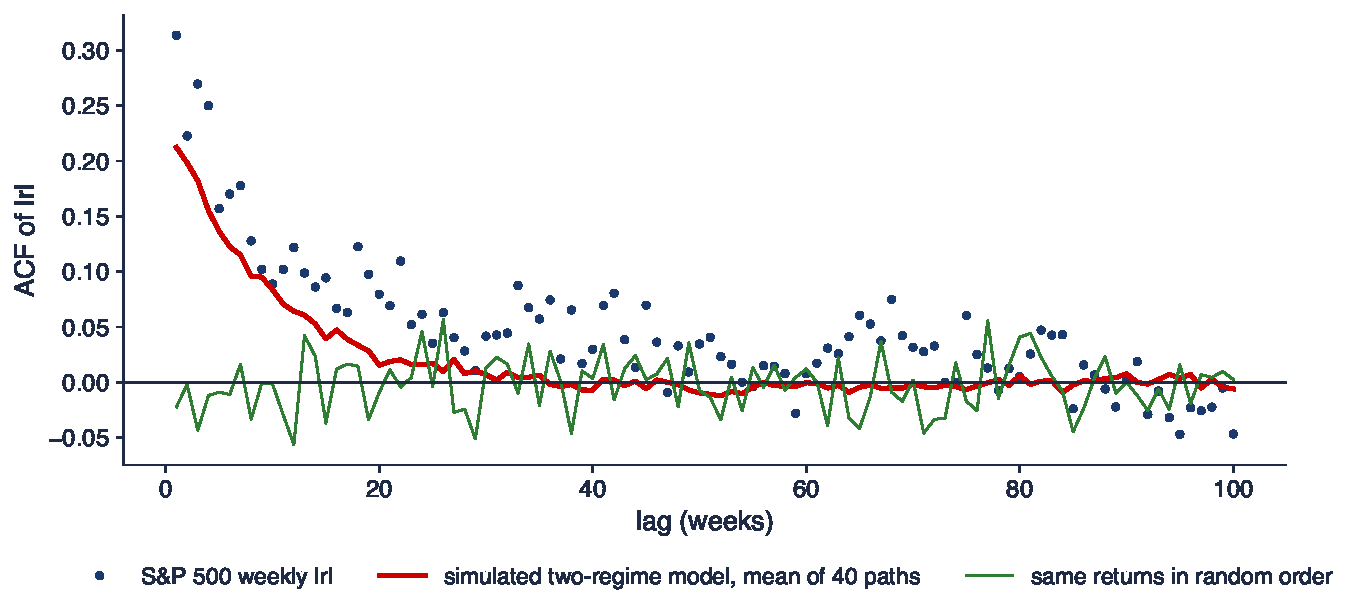
\includegraphics[width=0.97\textwidth,height=0.56\textheight,keepaspectratio]{tsa_ch10_regimes_memory.pdf}
\end{center}
\vspace{-0.25cm}
\begin{itemize}
    \item ACF a lui $|r_t|$ săptămînal pentru S\&P 500; ACF medie a 40 de serii simulate din modelul cu două regimuri estimat (varianță constantă în fiecare regim, fără GARCH); aceleași randamente în ordine aleatoare
\end{itemize}
\quantlet{TSA\_ch10\_volatility\_regimes}{\qlurl{TSA_ch10_volatility_regimes}}
\end{frame}

\begin{frame}{Interpretarea regimurilor simulate}
\itemsize{\small}
\begin{itemize}
    \item Datele: ACF a lui $|r_t|$ 0{,}31 la lagul 1, 0{,}06 la 26 de săptămîni; modelul cu regimuri: 0{,}21 și 0{,}01; ordinea aleatoare: nimic
    \begin{itemize}
        \item regimurile explică cea mai mare parte a volatility clustering-ului pe termen scurt, mai puțin din coada lungă a ACF
    \end{itemize}
    \item Estimatorul Whittle local $\hat d$ pentru $|r_t|$: 0{,}32 în date, 0{,}29 (SD 0{,}06) în seriile simulate cu regimuri, \ensuremath{-}0{,}05 în ordine aleatoare
    \begin{itemize}
        \item un GARCH(1,1) estimat pe seriile simulate dă în medie $\alpha + \beta = 0{,}91$ (15 serii), deși ele nu conțin GARCH
    \end{itemize}
    \item Persistența și memoria lungă a volatilității sînt compatibile cu regimurile: comparați modelele după verosimilitate și prognoze, nu după o singură statistică
\end{itemize}
\end{frame}

\begin{frame}{Recapitulare: modelele Markov switching}
\itemsize{\small}
\begin{itemize}
    \item $y_t = \mu_{S_t} + \varepsilon_t$, $S_t$ un lanț Markov; durate $1/(1 - p_{ii})$; ergodic $\pi_1 = (1-p_{22})/(2-p_{11}-p_{22})$
    \item Filtrul Hamilton: predicție cu $\mathbf{P}$, actualizare cu Bayes; netezitorul Kim pentru istorie
    \item PIB-ul SUA: modelul regăsește recesiunile NBER profunde; probabilitățile filtrate reacționează mai tîrziu
    \item Mai multe maxime, valorile extreme și rupturile de varianță pot schimba înțelesul unui „regim”
    \item Regimurile reproduc volatility clustering, persistența GARCH și memoria lungă aparentă
\end{itemize}
\end{frame}


%=============================================================================
\section{Contribuția posibilă a AI}
%=============================================================================

\begin{frame}{Contribuția posibilă a AI}
\itemsize{\small}
\begin{itemize}
    \item \textbf{Cod}: o primă versiune a unui filtru Kalman, a matricelor unui model nou, a unei estimări Markov switching cu multe valori de pornire
    \item \textbf{Explicații}: o a doua derivare a cîștigului, a stării de echilibru, a filtrului Hamilton
    \item \textbf{Explorare}: deviații PIB pentru multe țări din UE; regimuri pe multe piețe; un nowcast cu mulți indicatori
    \item Exemplu de prompt
    \begin{itemize}
        \item \aiprompt{Write Python code that downloads Romanian quarterly real GDP from Eurostat (namq\_10\_gdp, Q.CLV10\_MEUR.SCA.B1GQ.RO), fits UnobservedComponents with a smooth trend and an AR(2) cycle, compares the smoothed and the filtered cycle with the HP gap and with the Hamilton (2018) regression filter, and reports the revisions of the last eight quarters.}
    \end{itemize}
\end{itemize}
\end{frame}

\begin{frame}{Verificări necesare}
\itemsize{\small}
\begin{itemize}
    \item Simulați din parametri cunoscuți și verificați că acest cod îi regăsește (valorile pentru Nil din \refDK\ sînt un test bun)
    \item Filtrat sau netezit? Afirmațiile despre timp real cer estimări filtrate; un răspuns AI care folosește \texttt{smoothed} pentru o „prognoză” este greșit
    \item Duratele: $1/(1 - p_{ii})$, nu $p_{ii}/(1 - p_{ii})$; verificați convenția matricei de tranziție (rînduri sau coloane) în bibliotecă
    \item Markov switching: mai multe valori de pornire, schimbarea etichetelor, valori extreme care formează singure un regim
    \item Filtrul HP la capătul eșantionului: nu interpretați ultima deviație ca o estimare în timp real
    \item Fiecare referință citată: trebuie să existe; verificați DOI-ul
\end{itemize}
\end{frame}


%=============================================================================
\section{Rezumat}
%=============================================================================

\begin{frame}{Idei de reținut}
\itemsize{\small}
\begin{itemize}
    \item Forma în spațiul stărilor: o stare ascunsă $\alpha_t$ urmează un VAR(1) și este măsurată cu zgomot; ARMA, ETS, UC, TVP și modelele factoriale se scriu astfel
    \item Filtrul Kalman prezice și actualizează; cîștigul cîntărește datele în raport cu modelul; filtrul local level în starea de echilibru este SES
    \item Netezirea pentru istorie, filtrarea pentru timp real; verosimilitatea provine din erorile de predicție; valorile lipsă sînt ușor de tratat
    \item Deviațiile PIB depind de metodă și se revizuiesc puternic la capătul eșantionului
    \item Markov switching: probabilitățile regimurilor, durate $1/(1 - p_{ii})$; verificați ce înseamnă regimurile
\end{itemize}
\end{frame}

\begin{frame}{Formule de reținut}
\itemsize{\small}
{\renewcommand{\arraystretch}{1.35}\begin{center}
\footnotesize
\begin{tabular}{ll}
\toprule
\textbf{Mărimea} & \textbf{Formula} \\
\midrule
Forma în spațiul stărilor & $y_t = Z_t\alpha_t + \varepsilon_t$, \quad $\alpha_{t+1} = T\alpha_t + R\eta_t$ \\
Actualizarea & $v_t = y_t - Z_ta_t$, \quad $F_t = Z_tP_tZ_t' + H$, \quad $K_t = P_tZ_t'F_t^{-1}$, \quad $a_{t|t} = a_t + K_tv_t$ \\
Predicția & $a_{t+1} = Ta_{t|t}$, \quad $P_{t+1} = TP_{t|t}T' + RQR'$ \\
Starea de echilibru local level & $\bar P = \sigma^2_\varepsilon(q + \sqrt{q^2 + 4q})/2$, \quad $\alpha_{SES} = \bar K = \bar P/(\bar P + \sigma^2_\varepsilon)$ \\
Log-verosimilitatea & $-\frac12\sum_t(\log 2\pi + \log F_t + v_t^2/F_t)$ \\
Filtrul HP & $\min\sum(y_t - \tau_t)^2 + \lambda\sum(\Delta^2\tau_t)^2$, \quad $\lambda = \sigma^2_\varepsilon/\sigma^2_\zeta$ \\
Lanțul Markov & $E(D_i) = 1/(1 - p_{ii})$, \quad $\pi_1 = (1 - p_{22})/(2 - p_{11} - p_{22})$ \\
Filtrul Hamilton & $\Pr(S_t = j \mid Y_t) \propto f_j(y_t)\sum_i p_{ij}\Pr(S_{t-1} = i \mid Y_{t-1})$ \\
\bottomrule
\end{tabular}
\end{center}
}
\end{frame}

\begin{frame}{Autoevaluare}
\itemsize{\small}
\begin{itemize}
    \item \textbf{Întrebare}: local level cu $P_t = 3$, $\sigma^2_\varepsilon = 1$. Cît este cîștigul Kalman?
    \begin{itemize}
        \item \textbf{Răspuns}: $K_t = 3/(3 + 1) = 0{,}75$: noua observație primește ponderea 0,75
    \end{itemize}
    \item \textbf{Întrebare}: un model SES are $\alpha = 0{,}5$. Ce model local level se află în spatele lui?
    \begin{itemize}
        \item \textbf{Răspuns}: $q = \alpha^2/(1 - \alpha) = 0{,}25/0{,}5 = 0{,}5$
    \end{itemize}
    \item \textbf{Întrebare}: $p_{11} = 0{,}9$ într-un model cu două regimuri. Cît durează în medie regimul 1?
    \begin{itemize}
        \item \textbf{Răspuns}: $1/(1 - 0{,}9) = 10$ perioade
    \end{itemize}
    \item Urmează: \tsachlink{https://danpele.github.io/Time-Series-Analysis/RO/Cursuri/capitol11_foundation_models_serii_timp.pdf}{Capitolele 11}--\tsachlink{https://danpele.github.io/Time-Series-Analysis/RO/Cursuri/capitol14_modele_garch_multivariate.pdf}{14}, pentru studiu individual; \tsachlink{https://danpele.github.io/Time-Series-Analysis/RO/Cursuri/capitol15_recapitulare.pdf}{Capitolul 15}, recapitularea
\end{itemize}
\end{frame}


%=============================================================================
\section{Bibliografie}
%=============================================================================

\begin{frame}{Bibliografie (1/2)}
\itemsize{\scriptsize}
\begin{itemize}
    \item Chauvet, M., \& Piger, J. (2008). A comparison of the real-time performance of business cycle dating methods. \textit{Journal of Business \& Economic Statistics}, 26(1), 42--49. \href{https://doi.org/10.1198/073500107000000296}{doi:10.1198/073500107000000296}
    \item Diebold, F. X., \& Inoue, A. (2001). Long memory and regime switching. \textit{Journal of Econometrics}, 105(1), 131--159. \href{https://doi.org/10.1016/S0304-4076(01)00073-2}{doi:10.1016/S0304-4076(01)00073-2}
    \item Durbin, J., \& Koopman, S. J. (2012). \textit{Time Series Analysis by State Space Methods} (2nd ed.). Oxford University Press. \href{https://doi.org/10.1093/acprof:oso/9780199641178.001.0001}{doi:10.1093/acprof:oso/9780199641178.001.0001}
    \item Giannone, D., Reichlin, L., \& Small, D. (2008). Nowcasting: The real-time informational content of macroeconomic data. \textit{Journal of Monetary Economics}, 55(4), 665--676. \href{https://doi.org/10.1016/j.jmoneco.2008.05.010}{doi:10.1016/j.jmoneco.2008.05.010}
    \item Hamilton, J. D. (1989). A new approach to the economic analysis of nonstationary time series and the business cycle. \textit{Econometrica}, 57(2), 357--384. \href{https://doi.org/10.2307/1912559}{doi:10.2307/1912559}
    \item Hamilton, J. D. (1990). Analysis of time series subject to changes in regime. \textit{Journal of Econometrics}, 45(1--2), 39--70. \href{https://doi.org/10.1016/0304-4076(90)90093-9}{doi:10.1016/0304-4076(90)90093-9}
    \item Hamilton, J. D. (1994). \textit{Time Series Analysis}. Princeton University Press. \href{https://doi.org/10.2307/j.ctv14jx6sm}{doi:10.2307/j.ctv14jx6sm}
    \item Hamilton, J. D. (2018). Why you should never use the Hodrick--Prescott filter. \textit{The Review of Economics and Statistics}, 100(5), 831--843. \href{https://doi.org/10.1162/rest\_a\_00706}{doi:10.1162/rest\_a\_00706}
    \item Hamilton, J. D., \& Susmel, R. (1994). Autoregressive conditional heteroskedasticity and changes in regime. \textit{Journal of Econometrics}, 64(1--2), 307--333. \href{https://doi.org/10.1016/0304-4076(94)90067-1}{doi:10.1016/0304-4076(94)90067-1}
    \item Harvey, A. C. (1989). \textit{Forecasting, Structural Time Series Models and the Kalman Filter}. Cambridge University Press. \href{https://doi.org/10.1017/CBO9781107049994}{doi:10.1017/CBO9781107049994}
    \item Harvey, A. C., \& Jaeger, A. (1993). Detrending, stylized facts and the business cycle. \textit{Journal of Applied Econometrics}, 8(3), 231--247. \href{https://doi.org/10.1002/jae.3950080302}{doi:10.1002/jae.3950080302}
\end{itemize}
\end{frame}

\begin{frame}{Bibliografie (2/2)}
\itemsize{\scriptsize}
\begin{itemize}
    \item Hodrick, R. J., \& Prescott, E. C. (1997). Postwar U.S. business cycles: An empirical investigation. \textit{Journal of Money, Credit and Banking}, 29(1), 1--16. \href{https://doi.org/10.2307/2953682}{doi:10.2307/2953682}
    \item Huang, C., \& Petukhina, A. (2022). \textit{Applied Time Series Analysis and Forecasting with Python}. Springer. \href{https://doi.org/10.1007/978-3-031-13584-2}{doi:10.1007/978-3-031-13584-2}
    \item Hyndman, R. J., Koehler, A. B., Ord, J. K., \& Snyder, R. D. (2008). \textit{Forecasting with Exponential Smoothing: The State Space Approach}. Springer. \href{https://doi.org/10.1007/978-3-540-71918-2}{doi:10.1007/978-3-540-71918-2}
    \item Kalman, R. E. (1960). A new approach to linear filtering and prediction problems. \textit{Journal of Basic Engineering}, 82(1), 35--45. \href{https://doi.org/10.1115/1.3662552}{doi:10.1115/1.3662552}
    \item Kim, C.-J. (1994). Dynamic linear models with Markov-switching. \textit{Journal of Econometrics}, 60(1--2), 1--22. \href{https://doi.org/10.1016/0304-4076(94)90036-1}{doi:10.1016/0304-4076(94)90036-1}
    \item Kim, C.-J., \& Nelson, C. R. (1999). \textit{State-Space Models with Regime Switching: Classical and Gibbs-Sampling Approaches with Applications}. MIT Press. \href{https://doi.org/10.7551/mitpress/6444.001.0001}{doi:10.7551/mitpress/6444.001.0001}
    \item Lamoureux, C. G., \& Lastrapes, W. D. (1990). Persistence in variance, structural change, and the GARCH model. \textit{Journal of Business \& Economic Statistics}, 8(2), 225--234. \href{https://doi.org/10.1080/07350015.1990.10509794}{doi:10.1080/07350015.1990.10509794}
    \item Muth, J. F. (1960). Optimal properties of exponentially weighted forecasts. \textit{Journal of the American Statistical Association}, 55(290), 299--306. \href{https://doi.org/10.1080/01621459.1960.10482064}{doi:10.1080/01621459.1960.10482064}
    \item Rauch, H. E., Tung, F., \& Striebel, C. T. (1965). Maximum likelihood estimates of linear dynamic systems. \textit{AIAA Journal}, 3(8), 1445--1450. \href{https://doi.org/10.2514/3.3166}{doi:10.2514/3.3166}
    \item Shumway, R. H., \& Stoffer, D. S. (2017). \textit{Time Series Analysis and Its Applications} (4th ed.). Springer. \href{https://doi.org/10.1007/978-3-319-52452-8}{doi:10.1007/978-3-319-52452-8}
    \item Stock, J. H., \& Watson, M. W. (1989). New indexes of coincident and leading economic indicators. \textit{NBER Macroeconomics Annual}, 4, 351--394. \href{https://doi.org/10.1086/654119}{doi:10.1086/654119}
\end{itemize}
\end{frame}

\end{document}
